% Created 2016-08-01 Mon 22:52
\documentclass[9pt]{beamer}
\usepackage[utf8]{inputenc}
\usepackage[T1]{fontenc}
\usepackage{fixltx2e}
\usepackage{graphicx}
\usepackage{longtable}
\usepackage{float}
\usepackage{wrapfig}
\usepackage{soul}
\usepackage{textcomp}
\usepackage{marvosym}
\usepackage{wasysym}
\usepackage{latexsym}
\usepackage{amssymb}
\usepackage{hyperref}
\tolerance=1000
\mode<beamer>{\usetheme{Warsaw}}
\mode<beamer>{\setbeamertemplate{blocks}[rounded][shadow=false]}
\mode<beamer>{\addtobeamertemplate{block begin}{\pgfsetfillopacity{0.8}}{\pgfsetfillopacity{1}}}
\mode<beamer>{\setbeamercolor{structure}{fg=orange}}
\mode<beamer>{\setbeamercovered{transparent}}
\AtBeginSection[]{\begin{frame}<beamer>\frametitle{Topic}\tableofcontents[currentsection]\end{frame}}
\usepackage{subcaption}
\usepackage{multimedia}
\usepackage{tikz}
\usepackage{subfigure}
\usepackage{threeparttable}
\usetikzlibrary{shapes,arrows,shadows}
\usepackage{bm, amssymb, amsmath, array, pdfpages,graphicx}
\newcommand{\bv}[1]{\mathbf{#1}}
\newcommand{\diff}[2]{\frac{\partial #1}{\partial #2}}
\newcommand{\beq}[0]{\begin{equation}}
\newcommand{\eeq}[0]{\end{equation}}
\newcommand{\beqa}[0]{\begin{eqnarray}}
\newcommand{\eeqa}[0]{\end{eqnarray}}
\newcommand{\beqq}[0]{\begin{equation*}}
\newcommand{\eeqq}[0]{\end{equation*}}
\newcommand{\bs}[1]{\boldsymbol{#1}}
\newcommand{\ip}[2]{\langle #1, #2\rangle}
\providecommand{\alert}[1]{\textbf{#1}}

\title{Modeling and Uncertainty Quantification for Airfoil Icing}
\author{Anthony DeGennaro \newline Clarence W. Rowley III \newline Luigi Martinelli \newline Princeton University}
\date{JUP Quarterly Meeting \\ Princeton, NJ \\ April 2016}
\hypersetup{
  pdfkeywords={},
  pdfsubject={},
  pdfcreator={Emacs Org-mode version 7.9.3f}}

\begin{document}

\maketitle

\begin{frame}
\frametitle{Outline}
\setcounter{tocdepth}{3}
\tableofcontents
\end{frame}



% Define my settings

\graphicspath{{Figures/}}
% Add Princeton shield logo
\addtobeamertemplate{frametitle}{}{%
\begin{tikzpicture}[remember picture,overlay]
\node[anchor=north east,yshift=2pt] at (current page.north east) {
\includegraphics[height=0.7cm]{Shield}};
\end{tikzpicture}}
%


\institute{Princeton University}

\section{Motivation/Background}
\label{sec-1}
\begin{frame}
\frametitle{Introduction}
\label{sec-1-1}

\begin{columns}[c]
  \column{0.5\textwidth}
    \centering
    {\bf Wing icing deteriorates aerodynamics}
    \begin{itemize}
      \item{Leading edge flow separation bubble}
      \item{Lower lift, higher drag}
      \item{Unpredictable stall}
    \end{itemize}
  \column{0.5\textwidth}
    \vspace*{-0.0cm}\begin{figure}
    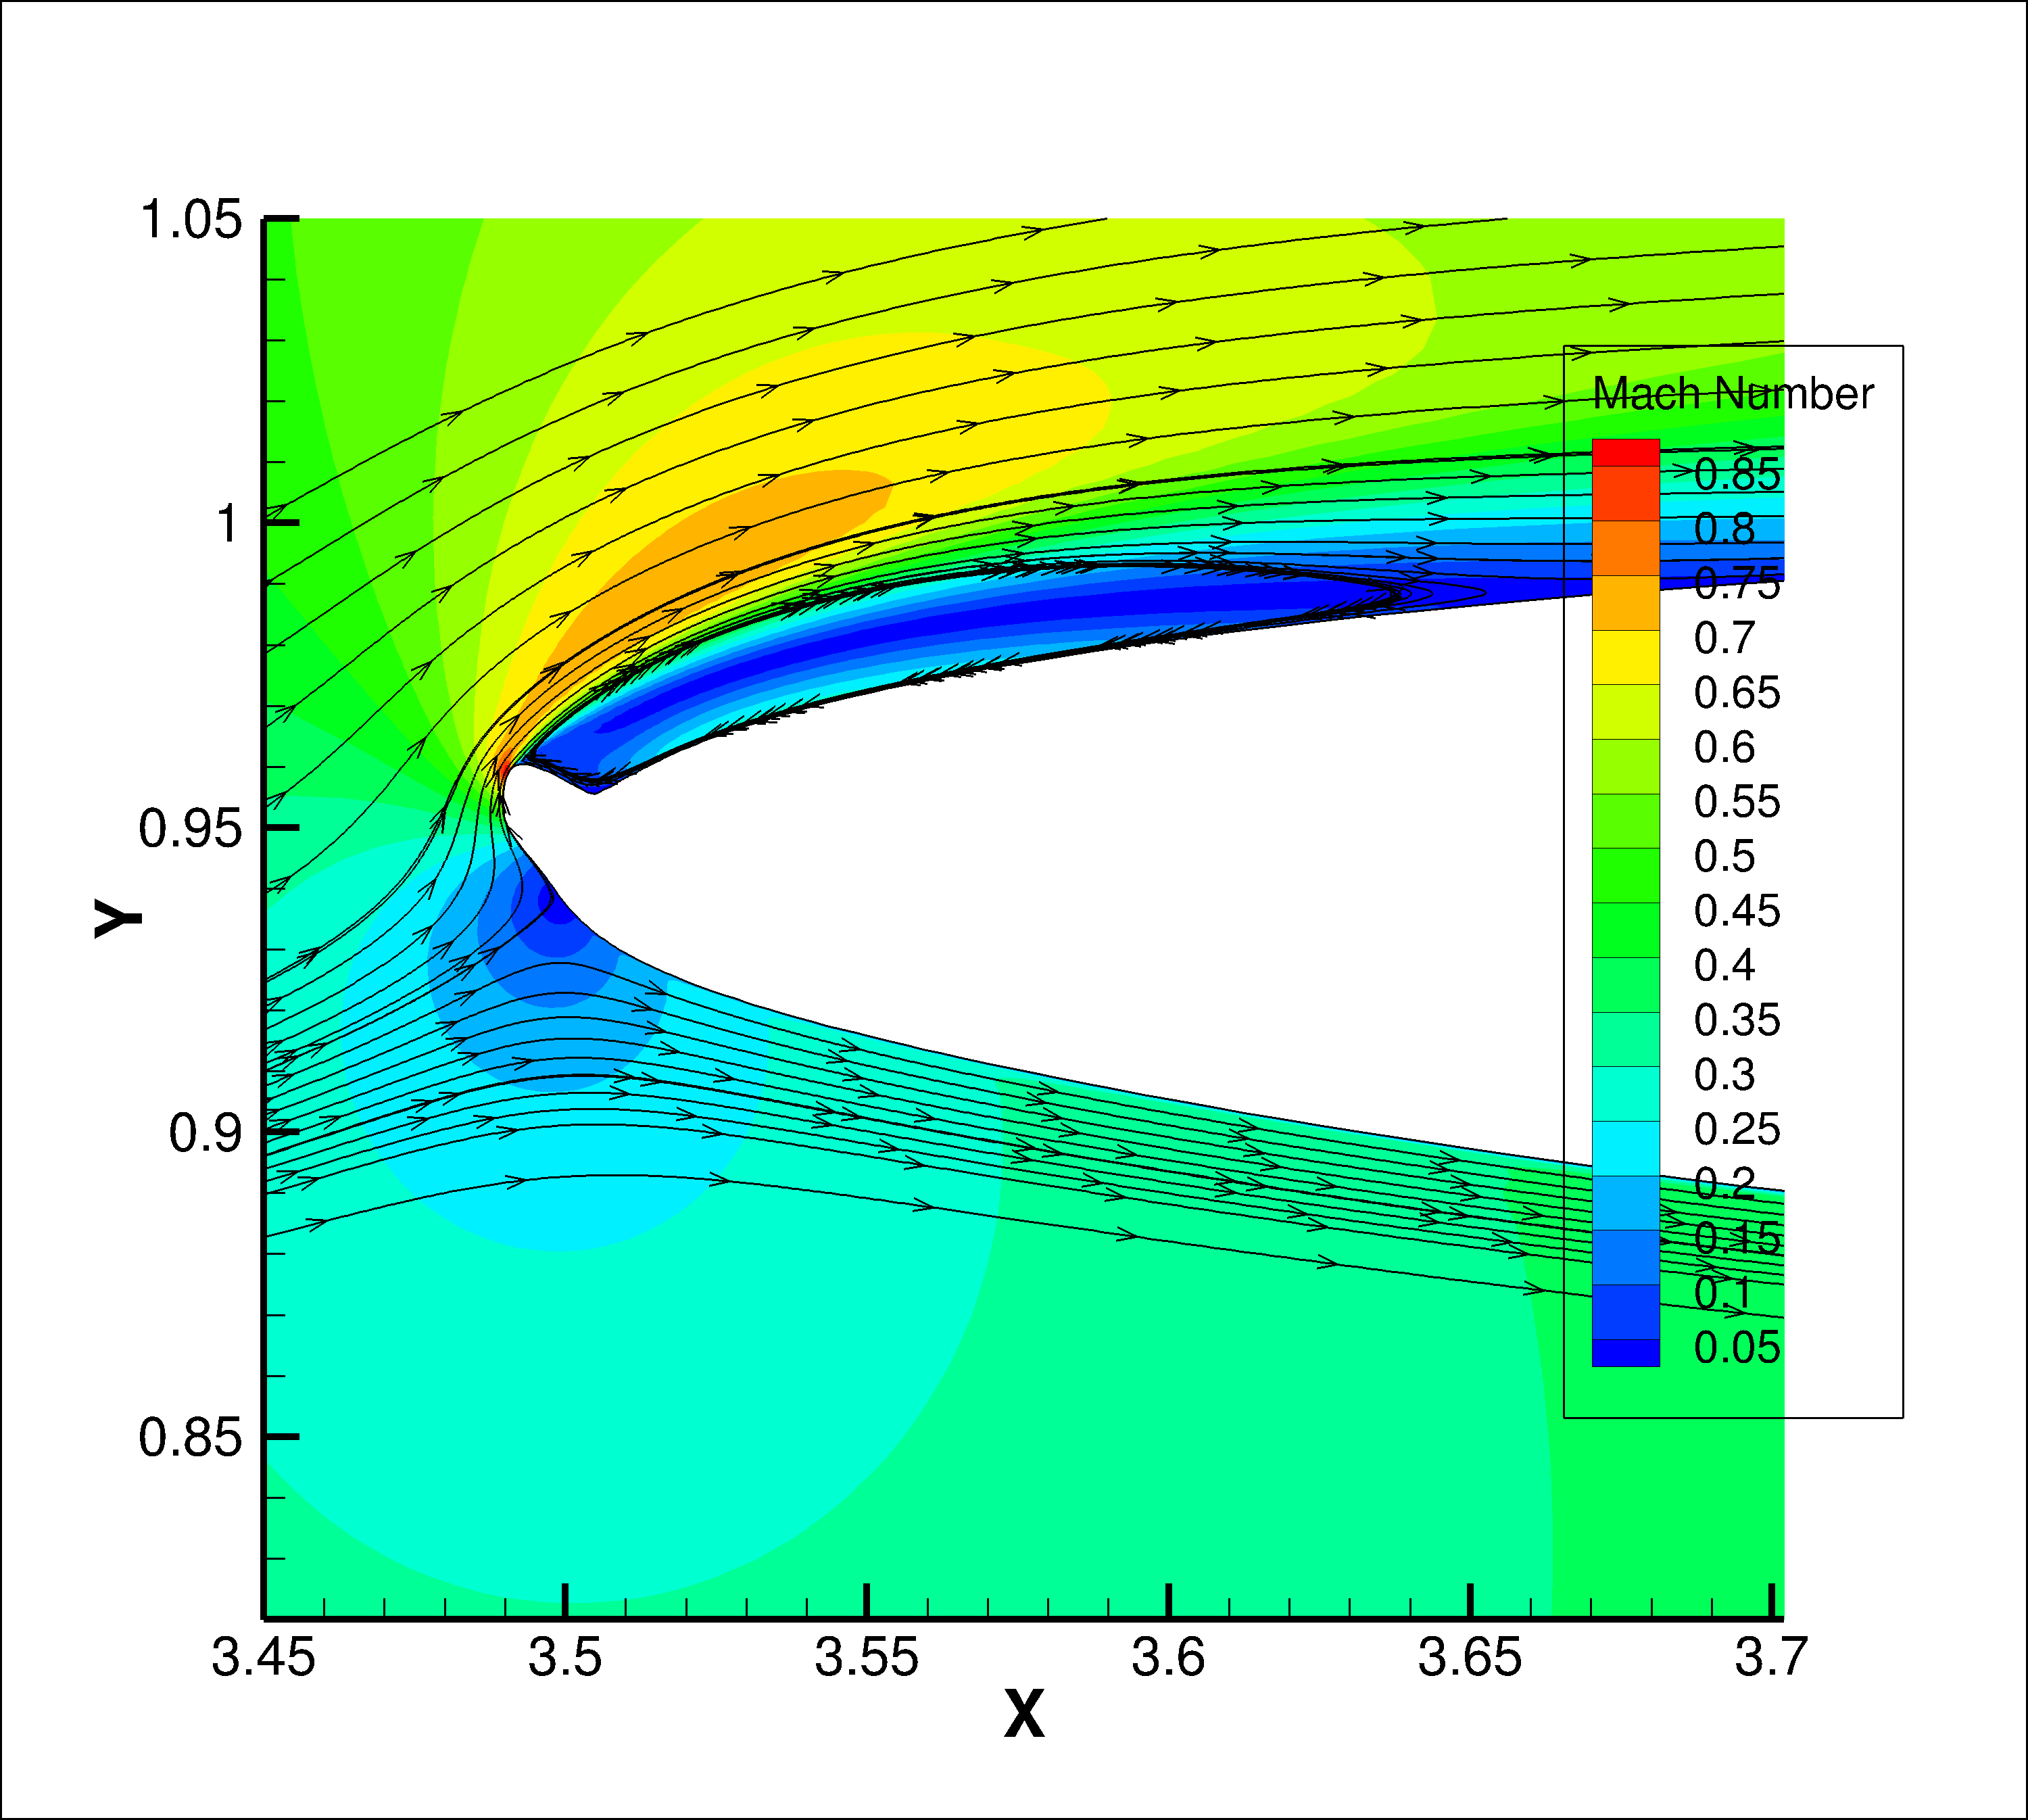
\includegraphics[width=1\textwidth]{BadHorn.png}
    \caption{Leading edge horn separation}
    \end{figure}
  \end{columns}
\end{frame}
\begin{frame}
\frametitle{Introduction}
\label{sec-1-2}

\textbf{Significant ice shape variation, sensitivity to physical parameters}\footnote{Addy, H.E. \emph{Ice Accretions and Icing Effects for Modern Airfoils}. NASA TR 2000-210031.
 }
\begin{itemize}
\item Complex physics (aero-thermodynamics, macro/micro scale physics)
\item Uncertainty in physical parameters
\item Nondeterministic variation (``same conditions, different shapes'')
\end{itemize}

\vspace*{-0.0cm}\begin{figure}
      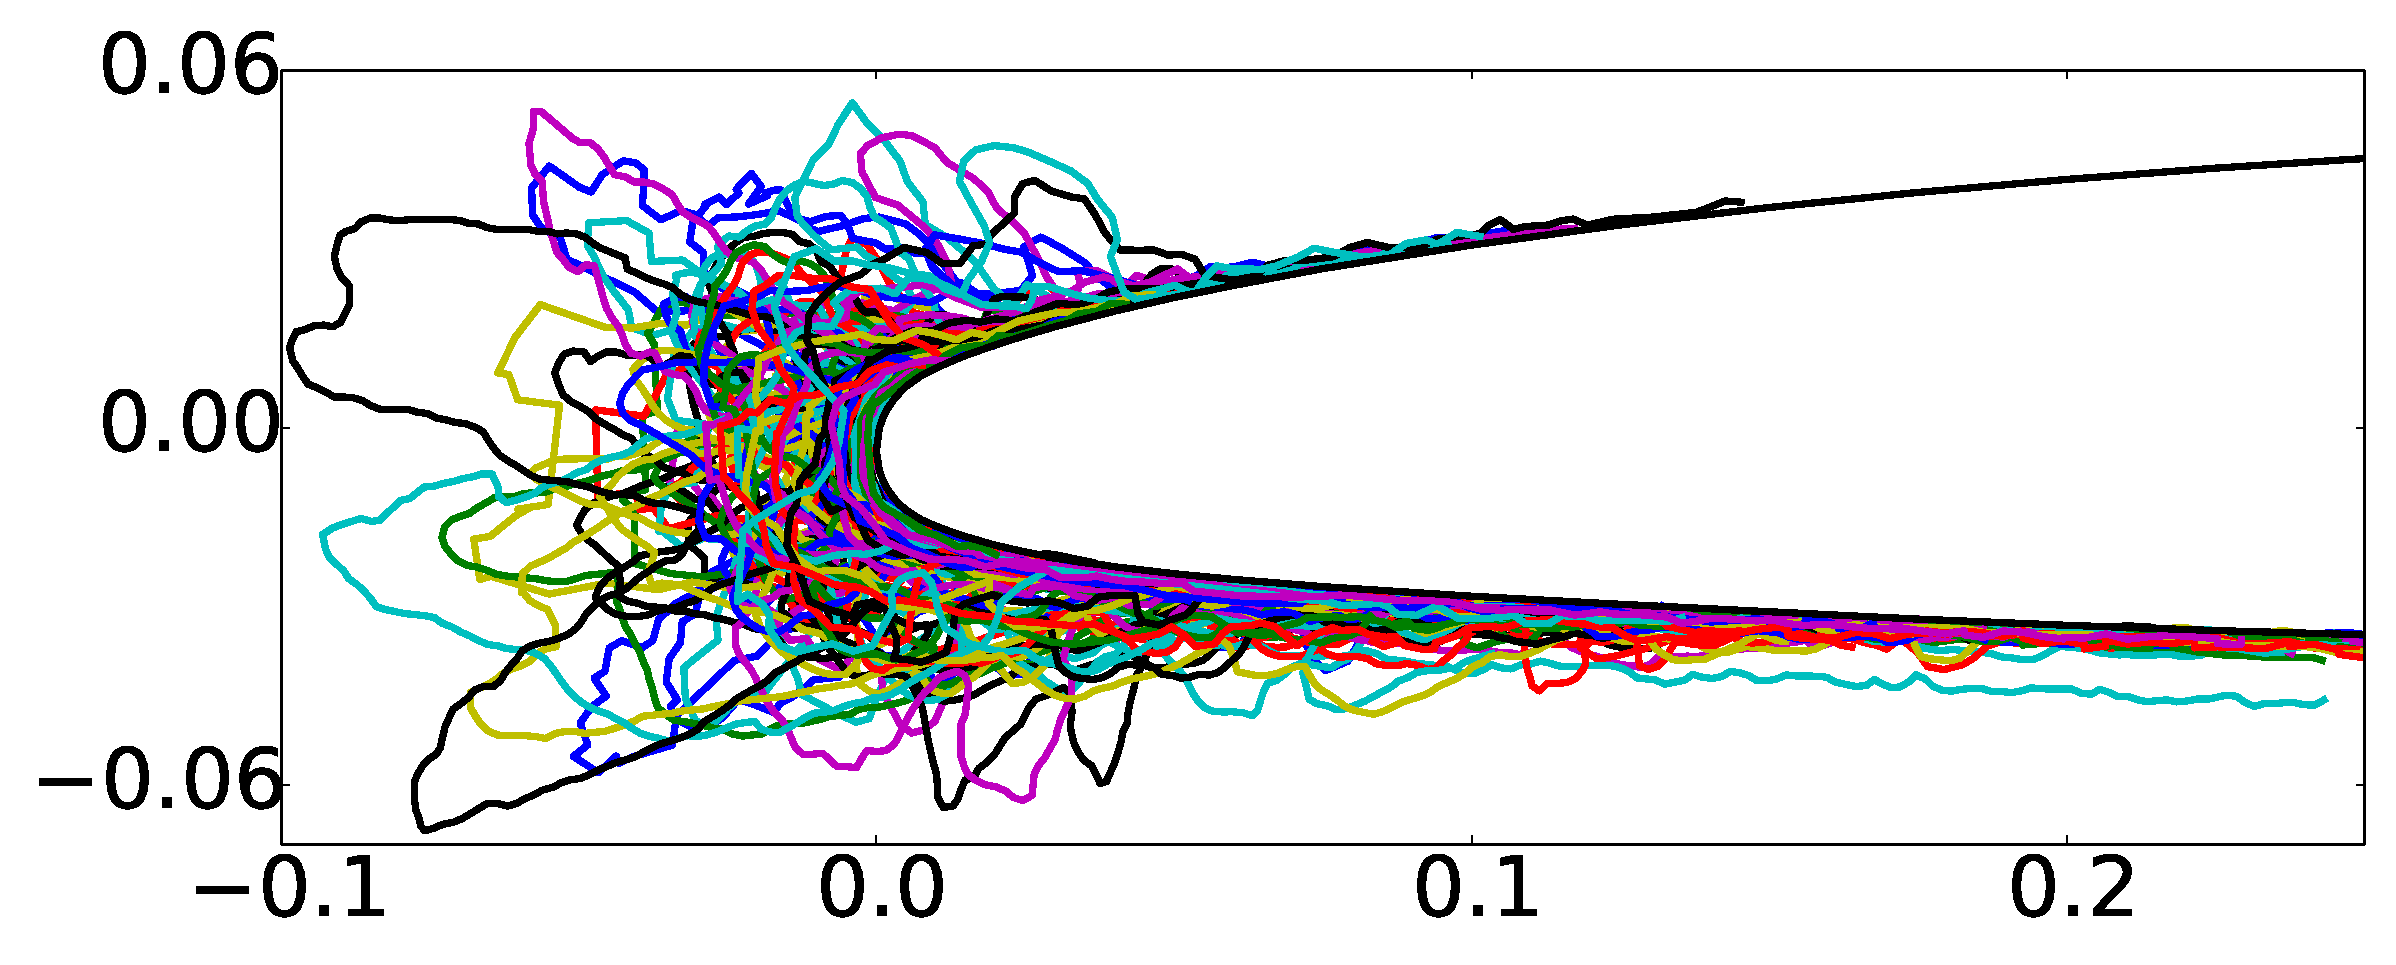
\includegraphics[width=0.75\textwidth]{GlobalDataSet}
      \caption{Wind tunnel experimental ice shapes}
\end{figure}
\end{frame}
\begin{frame}
\frametitle{Introduction}
\label{sec-1-3}

\textbf{Different types of ice accretion}\footnote{Beaugendre et. al. \emph{Development of a Second Generation In-Flight Simulation Code}. J. Fluids Engineering, 2006.
 }
\begin{itemize}
\item ``Rime'' ice: cold temperature, low liquid water content
\item ``Horn'' ice: warm temperature, high liquid water content
\item Uncertainty in physical conditions can create uncertainty in performance
\end{itemize}

\vspace*{-0.0cm}\begin{figure}
      \subfigure[Rime Ice]{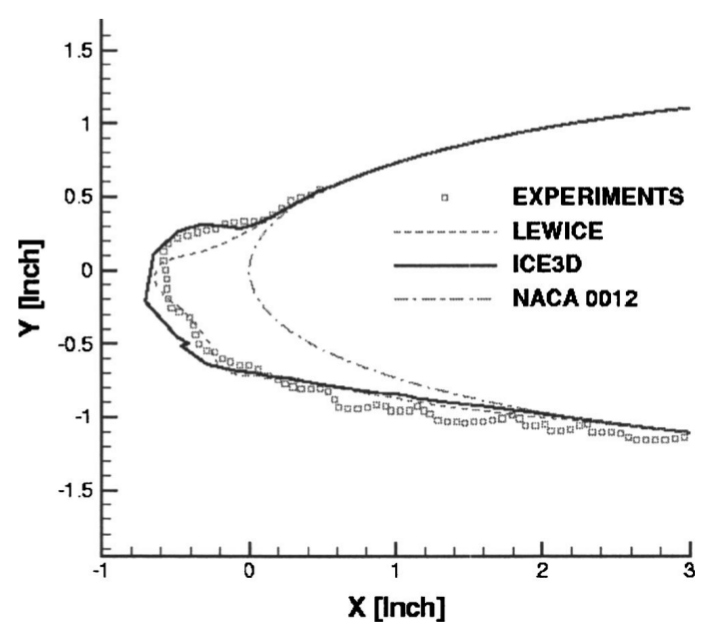
\includegraphics[width=0.4\textwidth]{Habashi2006Rime.png}}
      \subfigure[Horn Ice]{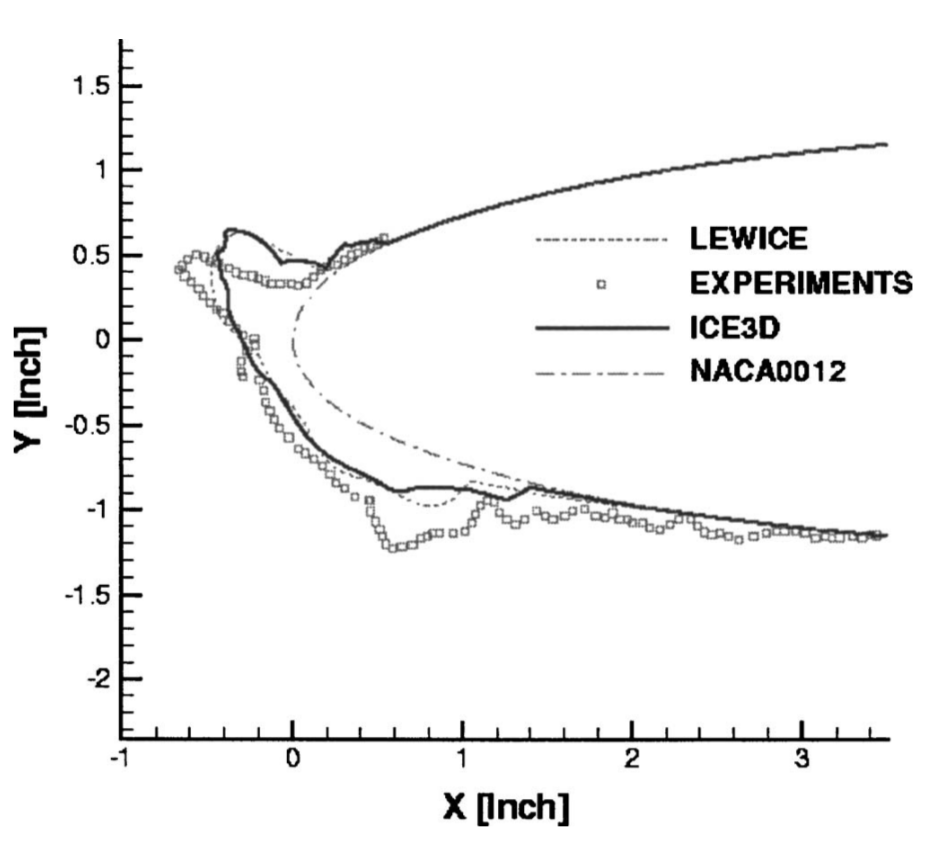
\includegraphics[width=0.4\textwidth]{Habashi2006Horn.png}}
 
\end{figure}
\end{frame}
\begin{frame}
\frametitle{Introduction}
\label{sec-1-4}

\textbf{Observations}
\begin{itemize}
\item Many experimental ice accretion results exist, but no one has
  modeled this data or inferred anything from it
\item Numerical methods/codes exist, but no one has systematically quantified
  statistical effects of parametric uncertainty in physics
\end{itemize}
\textbf{Questions}
\begin{itemize}
\item Can we infer/identify prominent ice shape features from database of shapes?
\item We can link physical information about data to ice shape features?
\item Can we create a statistical modeling of icing using only data?
\item Can we investigate parametric uncertainty in numerical icing codes?
\end{itemize}
\end{frame}
\begin{frame}
\frametitle{Introduction}
\label{sec-1-5}

\textbf{Research Goals}

\begin{itemize}
\item Data-driven, equation-free model of ice accretion
\begin{itemize}
\item Model ice accretion using \emph{only} data, no physics
\item Study random ice shapes corresponding to a range of icing conditions
\item Could be used to benchmark/correct numerical calculations
\item Could be used to explore \emph{non-deterministic} ice shape variations
\end{itemize}
\item Computational model of ice accretion
\begin{itemize}
\item Build numerical code to calculate ice accretion given physical inputs
\item Compute ice shape for a range of physical conditions
\item Perform parametric UQ and study effects on aerodynamic performance
\end{itemize}
\end{itemize}
\end{frame}
\begin{frame}
\frametitle{Introduction}
\label{sec-1-6}

\textbf{Research Approach}

\begin{itemize}
\item Data-driven, equation-free modeling of ice accretion
\begin{itemize}
\item Collect large number of ice shapes into a database
\item Model database shape features using Proper Orthogonal Decomposition (POD)
\item Link physical information to shape features
\item Build a purely data-driven, statistical ice accretion model (\emph{no equations})
\item Perform parametric UQ, study performance variations, etc.
\end{itemize}
\item Computational model of ice accretion
\begin{itemize}
\item Build droplet advection/impact simulator (C++)
\item Build icing thermodynamics simulator (C++)
\item Interface code with aerodynamic solver (FLO103)
\item Perform parametric UQ, study performance variations, etc.
\end{itemize}
\end{itemize}
\end{frame}
\section{Data-Based UQ}
\label{sec-2}
\begin{frame}
\frametitle{Dataset}
\label{sec-2-1}

\vspace*{-0.0cm}\begin{figure}
      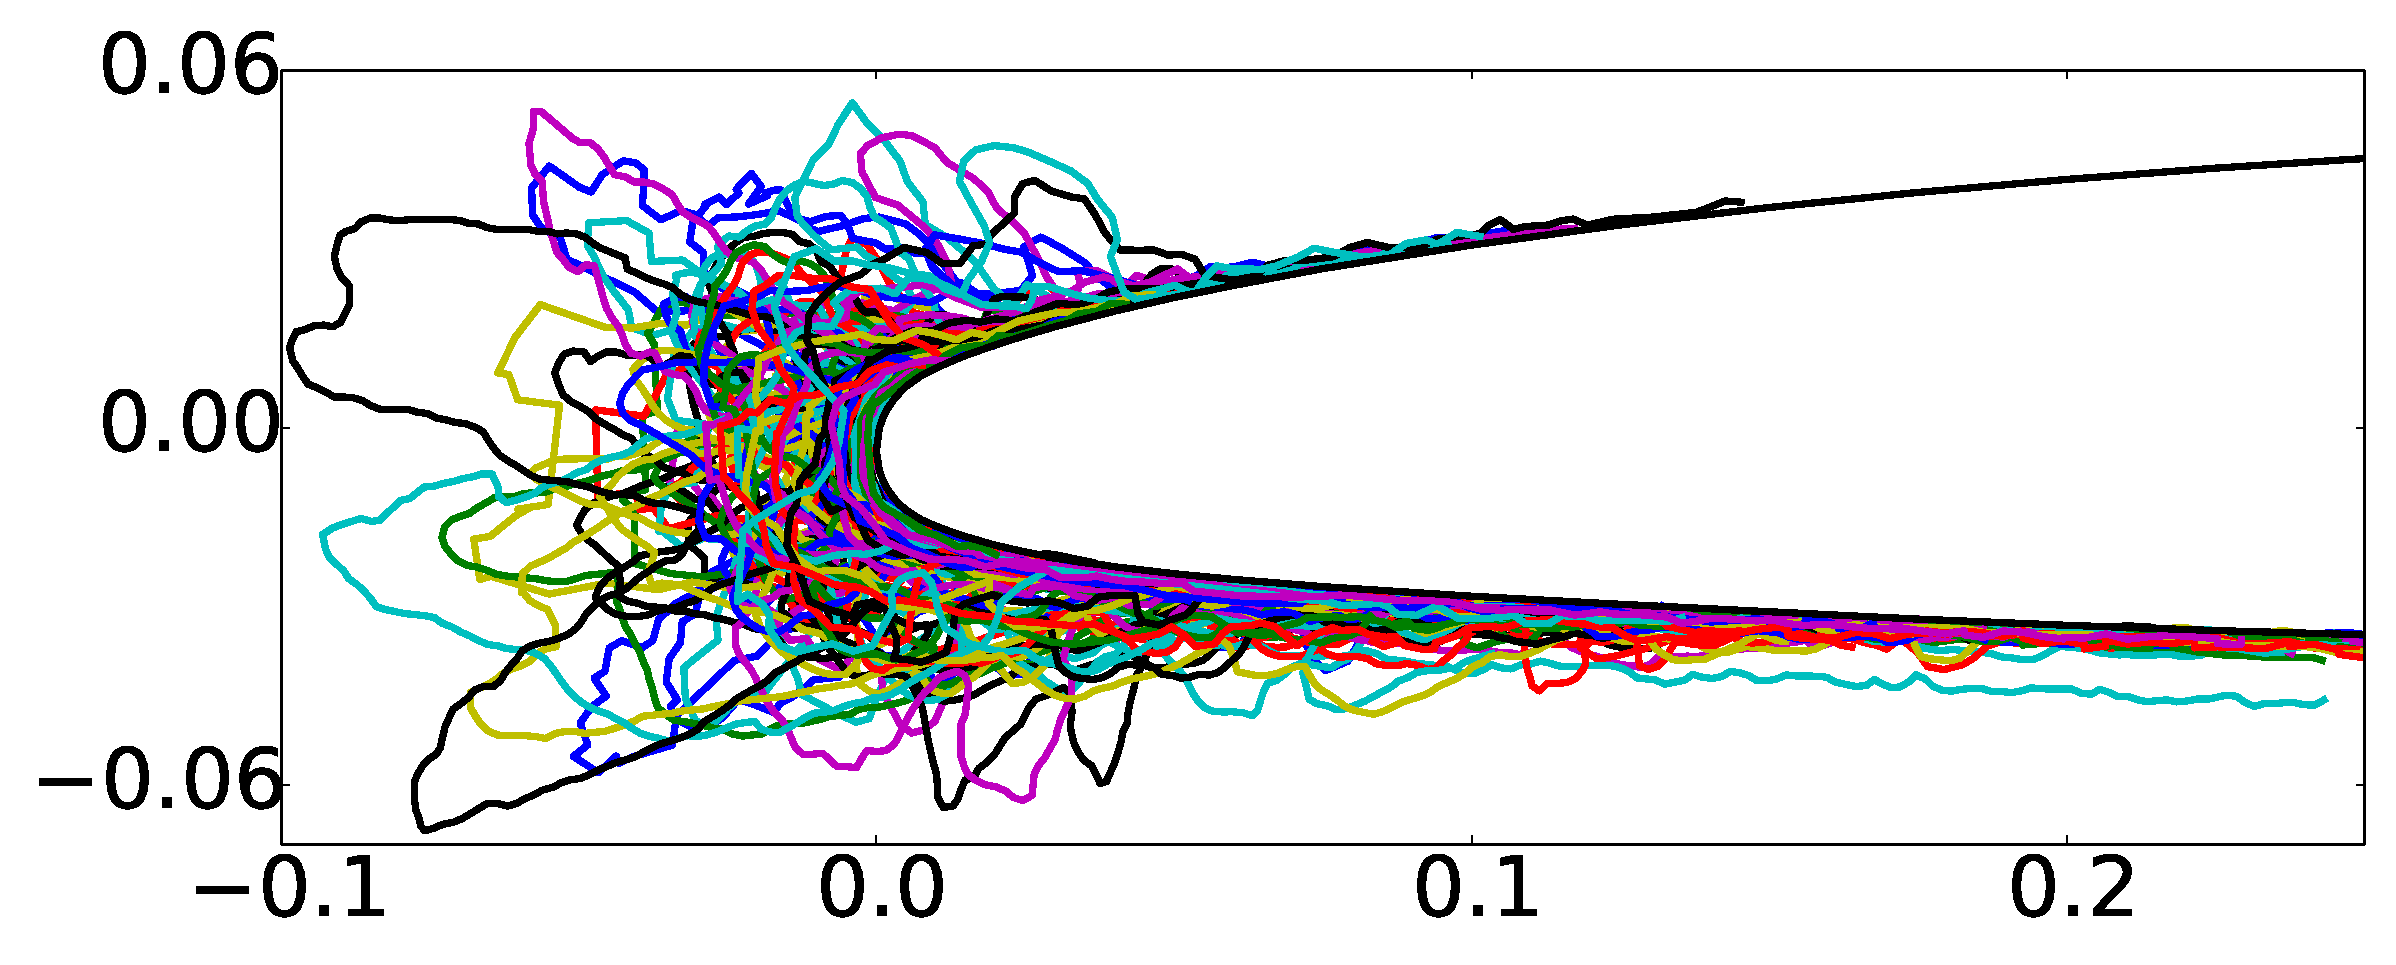
\includegraphics[width=0.5\textwidth]{GlobalDataSet}
      \caption{Wind tunnel experimental ice shapes}
\end{figure}
\begin{itemize}
\item Dataset consists of 145 experimental ice shapes
\item Obtained in icing wind tunnel at NASA Glenn\footnotemark[1]
\item Representative of a wide variety of icing conditions (temperature,
  LWC, accretion time, etc.)
\end{itemize}
  
\end{frame}
\begin{frame}
\frametitle{Data-Driven Model}
\label{sec-2-2}

\vspace*{-0.0cm}\begin{figure}
      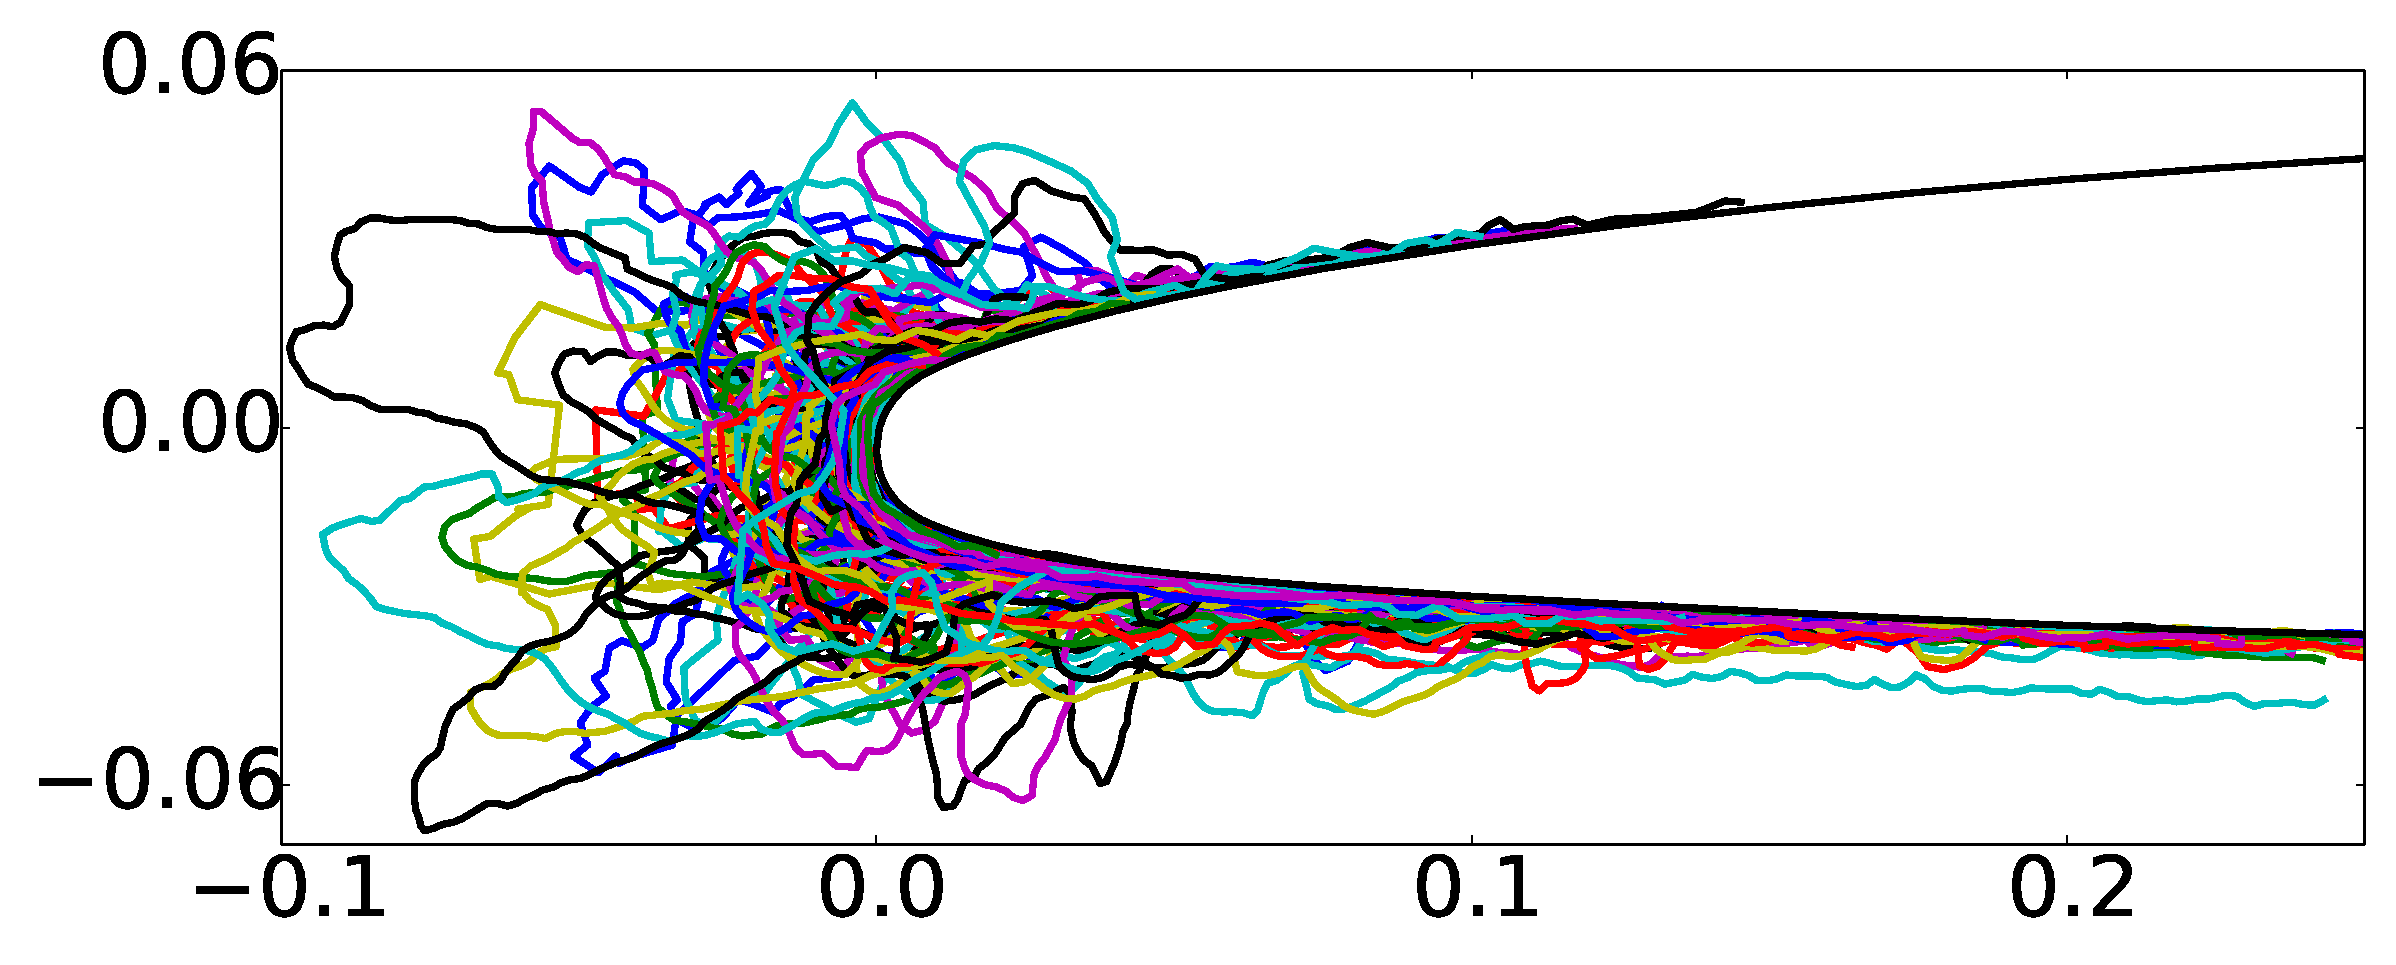
\includegraphics[width=0.5\textwidth]{GlobalDataSet}
      \caption{Wind tunnel experimental ice shapes}
\end{figure}
\textbf{Goal:} Make a purely data-driven model of icing (no equations)

\textbf{Approach:}
\begin{itemize}
\item Build low-dimensional model of shape using POD
\item Correlate POD coefficients to temperature, accretion time, LWC
\item Generate random ice shapes corresponding to given conditions
\end{itemize}
\end{frame}
\begin{frame}
\frametitle{Proper Orthogonal Decomposition (POD)}
\label{sec-2-3}

\textbf{Goal/Utility}
\begin{itemize}
\item Statistical analysis tool
\item Extracts linear, orthogonal basis that optimally explains dataset
\end{itemize}
\textbf{Method}
\begin{itemize}
\item Singular value decomposition of data matrix gives POD modes and eigenvalues
\end{itemize}
\begin{equation*}
\begin{aligned}
\mathbf{X} &=
 \begin{bmatrix}
   \vline & & \vline \\
   x_1 & \cdots & x_S \\
   \vline & & \vline \\
 \end{bmatrix}\\
 \bv{X} &= \Phi\Sigma\bv{V^*}\\
 x &\approx \sum_i^{M} c_i \phi_i
\end{aligned}
\end{equation}
\end{frame}
\begin{frame}
\frametitle{POD Eigenvalues}
\label{sec-2-4}

\vspace*{-0.0cm}\begin{figure}
      \subfigure[Magnitude.]{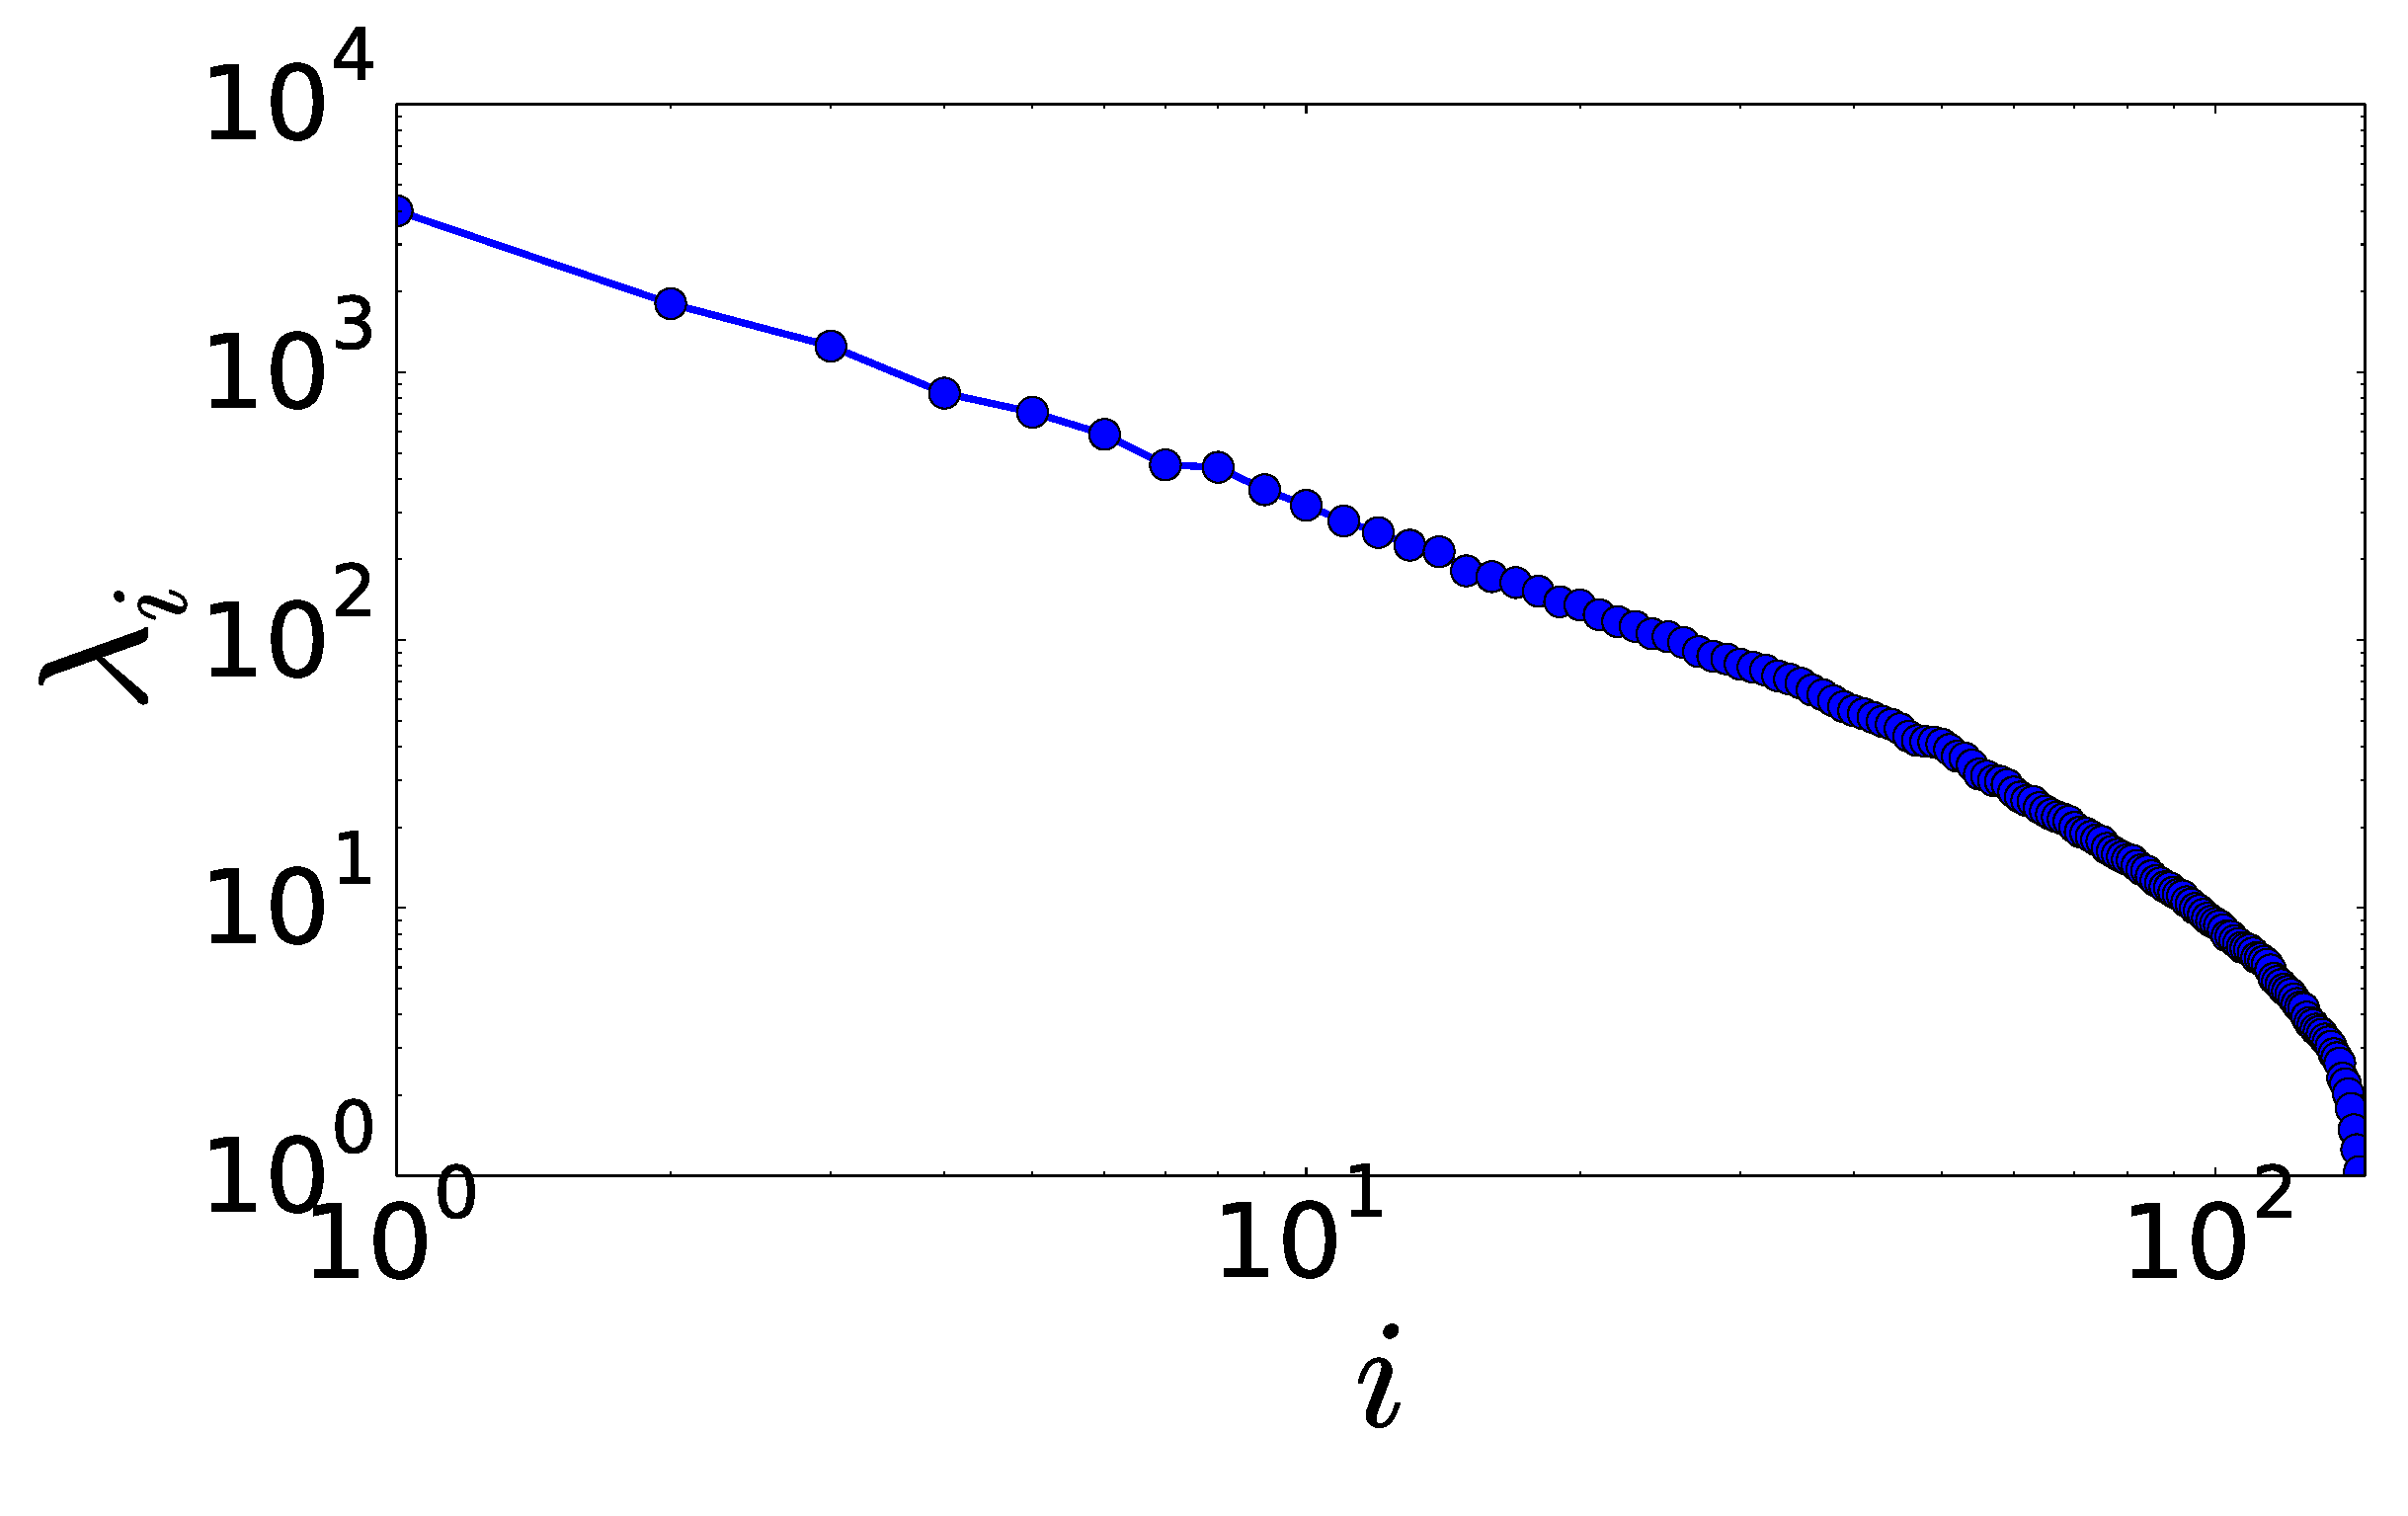
\includegraphics[width=0.4\textwidth]{PODevals.eps}}
      \subfigure[Cumulative sum.]{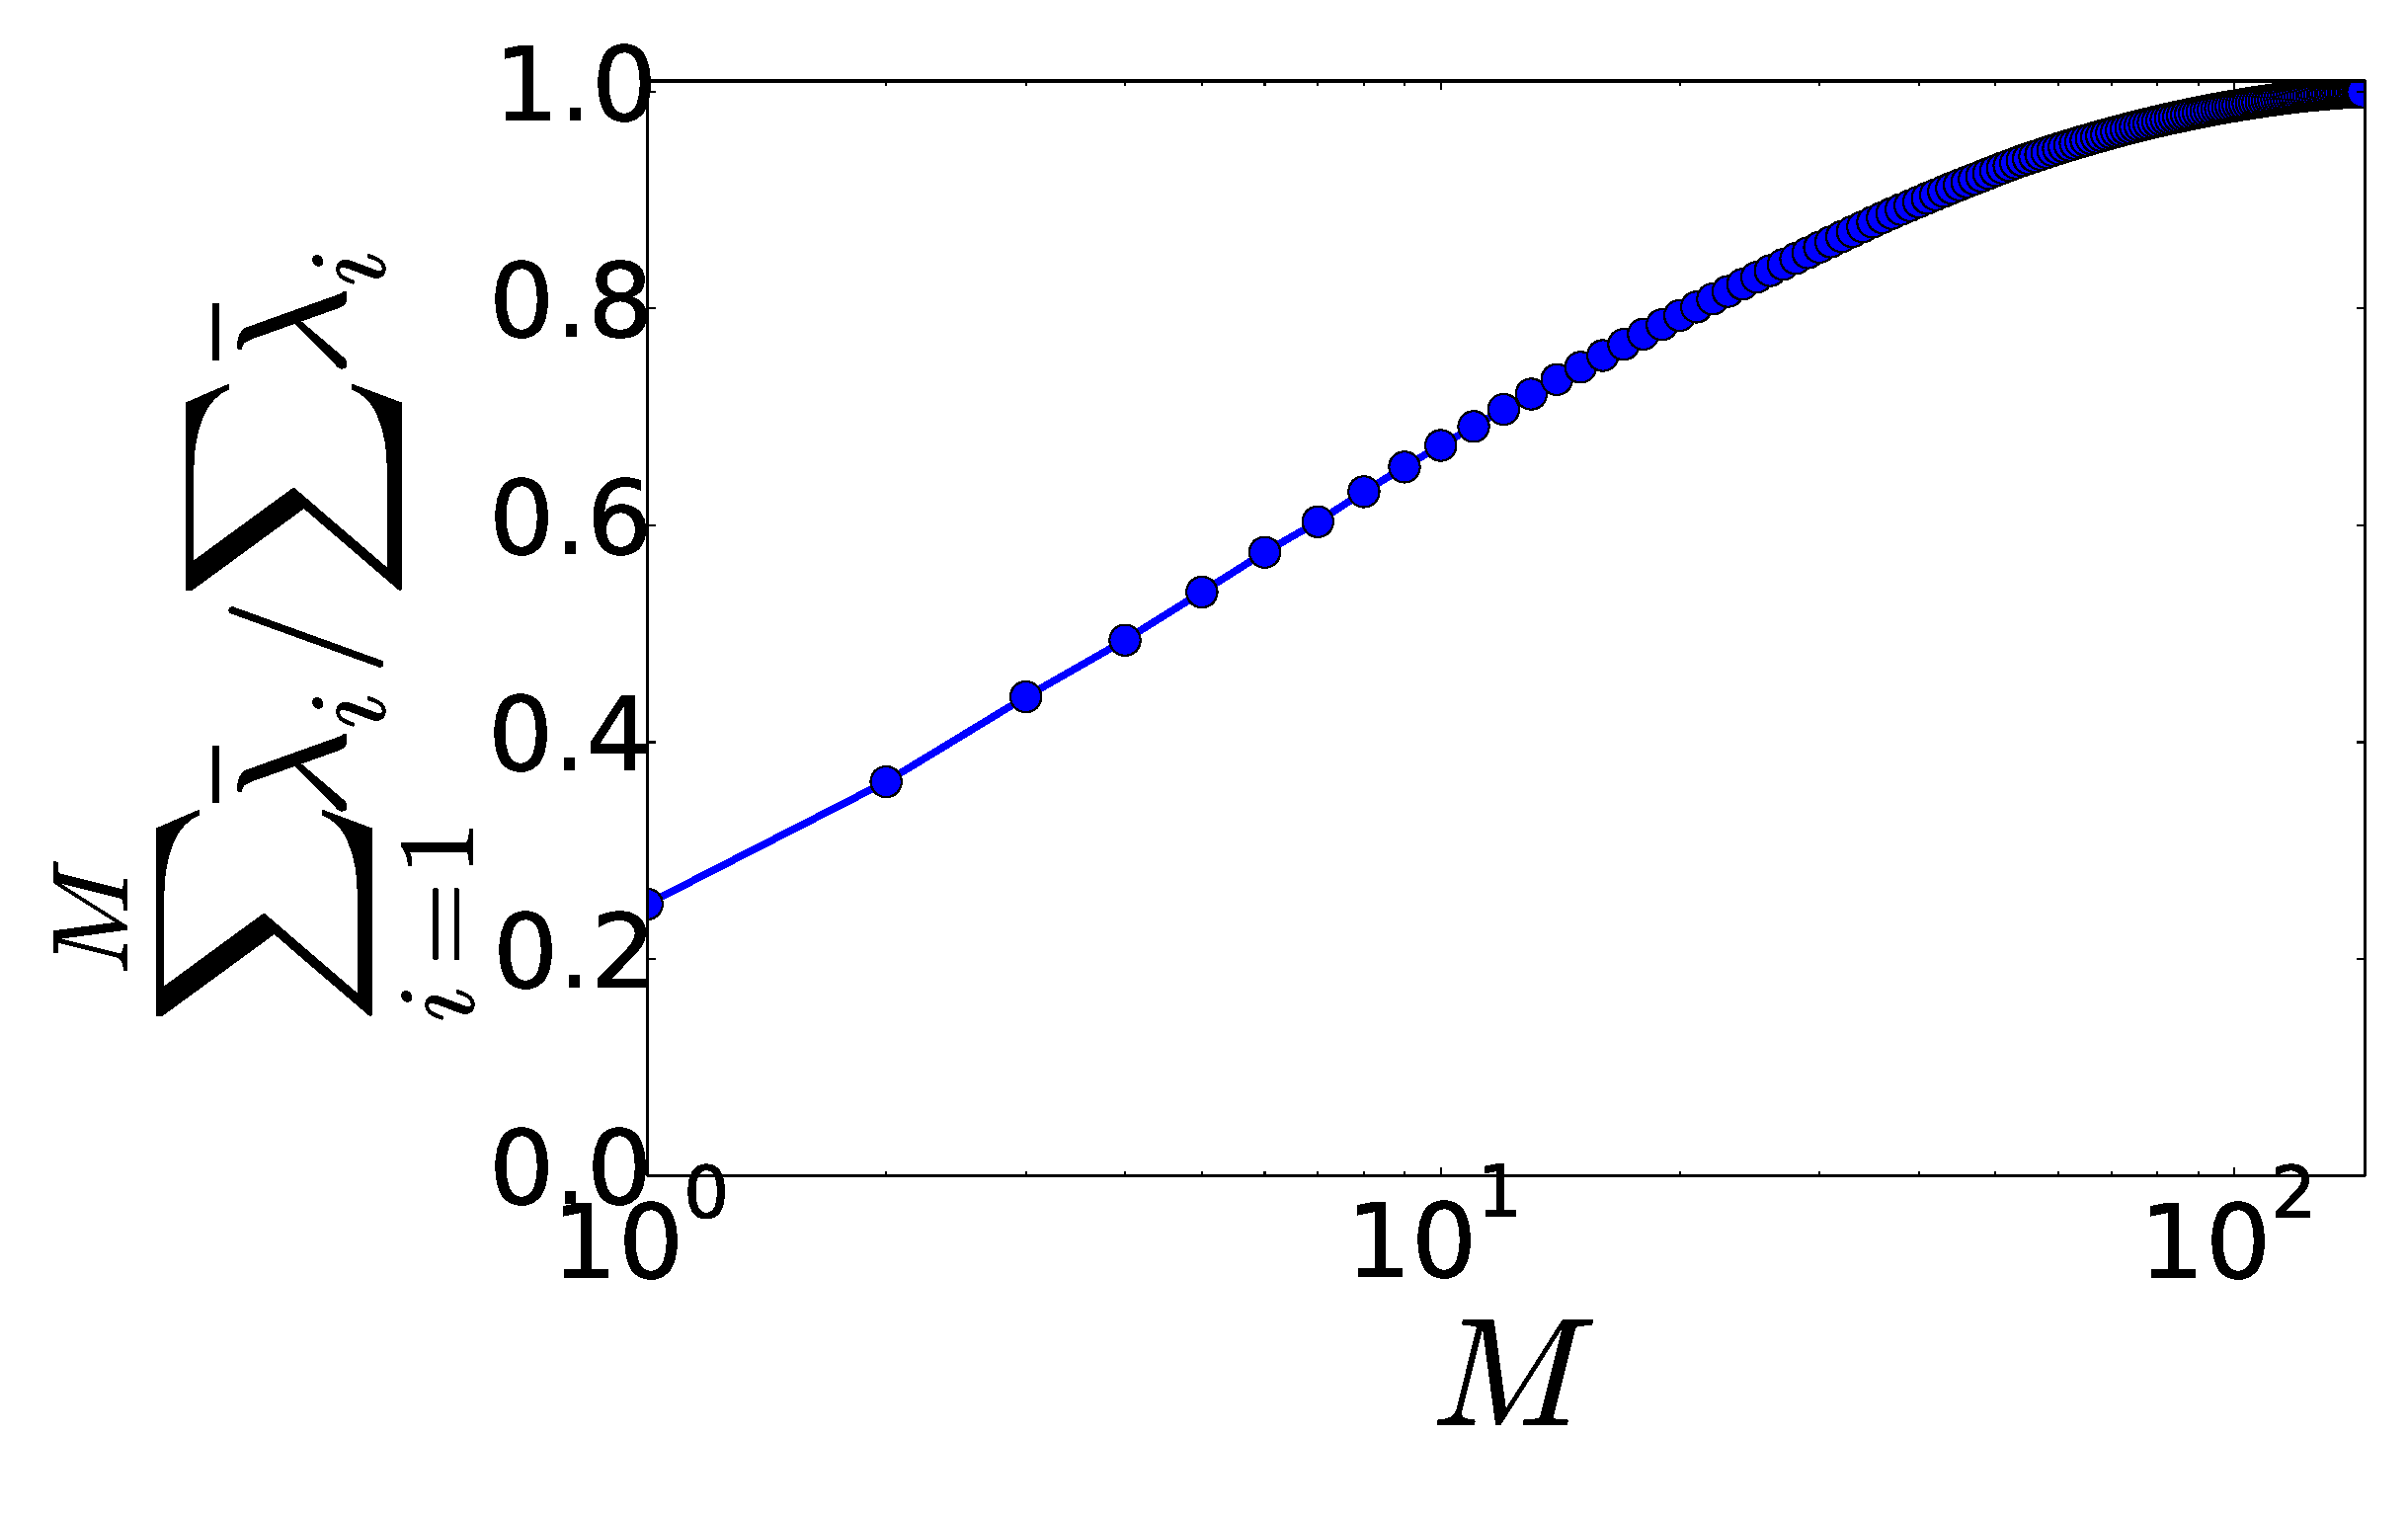
\includegraphics[width=0.4\textwidth]{CumsumPODevals.eps}}
      \caption{POD eigenvalues.}
\end{figure}

\begin{itemize}
\item 2/3 of cumulative sum contained in first 10 modes
\item 2/3 of statistical variation contained in first 10 modes
\item Truncate model at 10 modes
\end{itemize}
\end{frame}
\begin{frame}
\frametitle{POD Modes}
\label{sec-2-5}

\vspace*{0.75cm}\begin{figure}
      \vspace*{-1.75cm}\subfigure{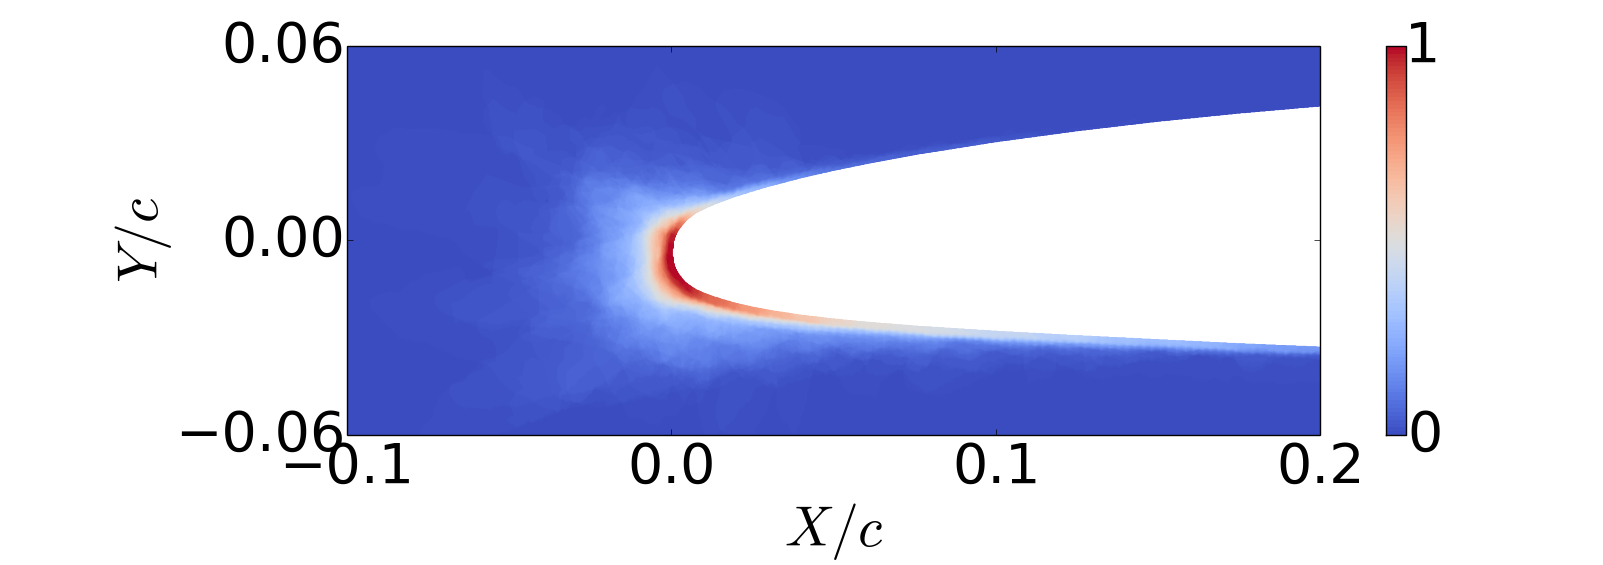
\includegraphics[width=0.4\textwidth]{MEAN}} \\
      \vspace*{-0.75cm}\subfigure{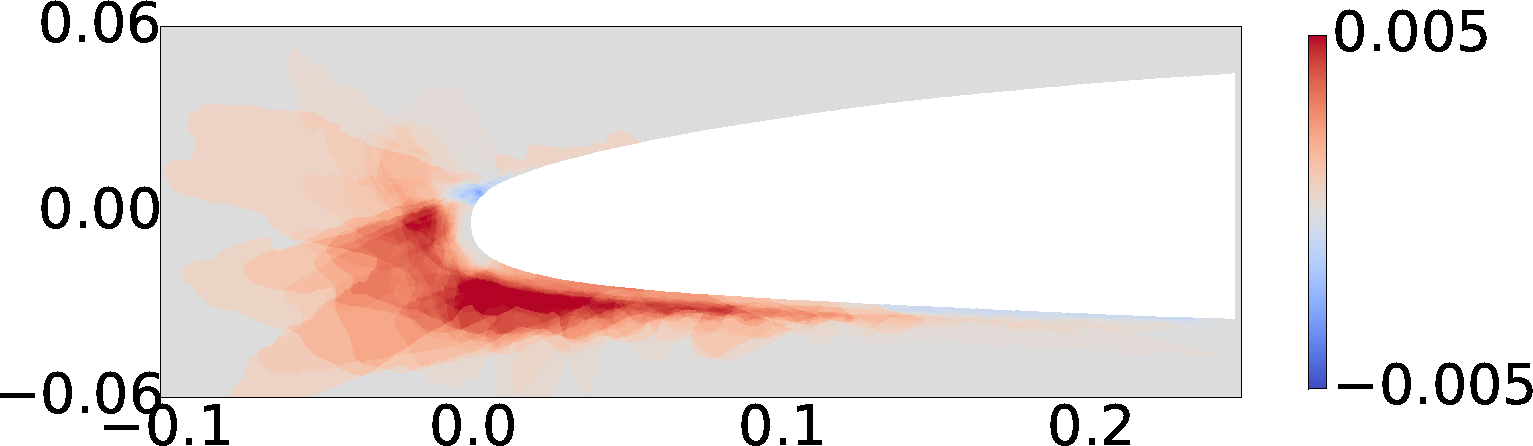
\includegraphics[width=0.4\textwidth]{MODE1}}
      \vspace*{-0.75cm}\subfigure{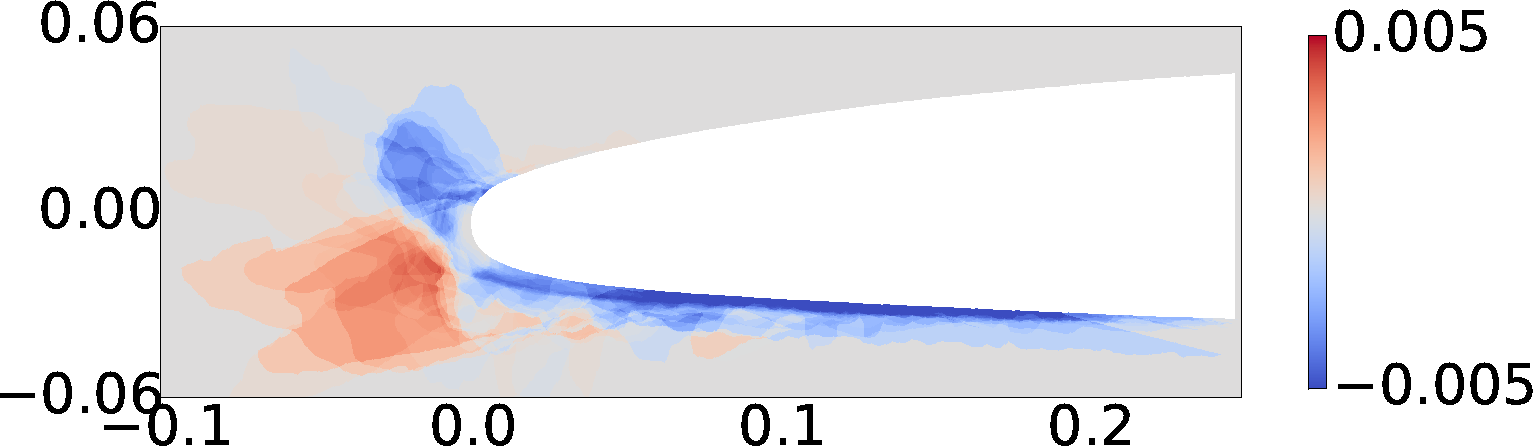
\includegraphics[width=0.4\textwidth]{MODE2}}
      \vspace*{-0.75cm}\subfigure{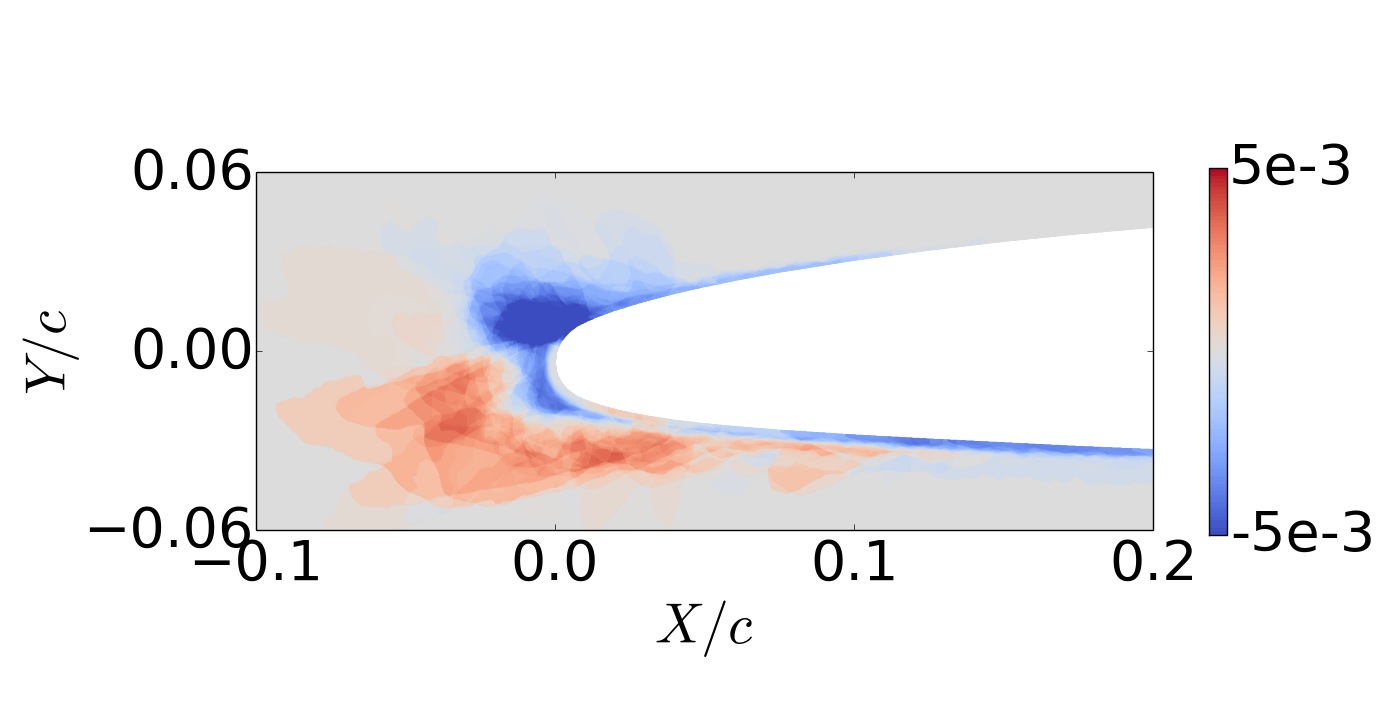
\includegraphics[width=0.4\textwidth]{MODE3}}
      \vspace*{-0.75cm}\subfigure{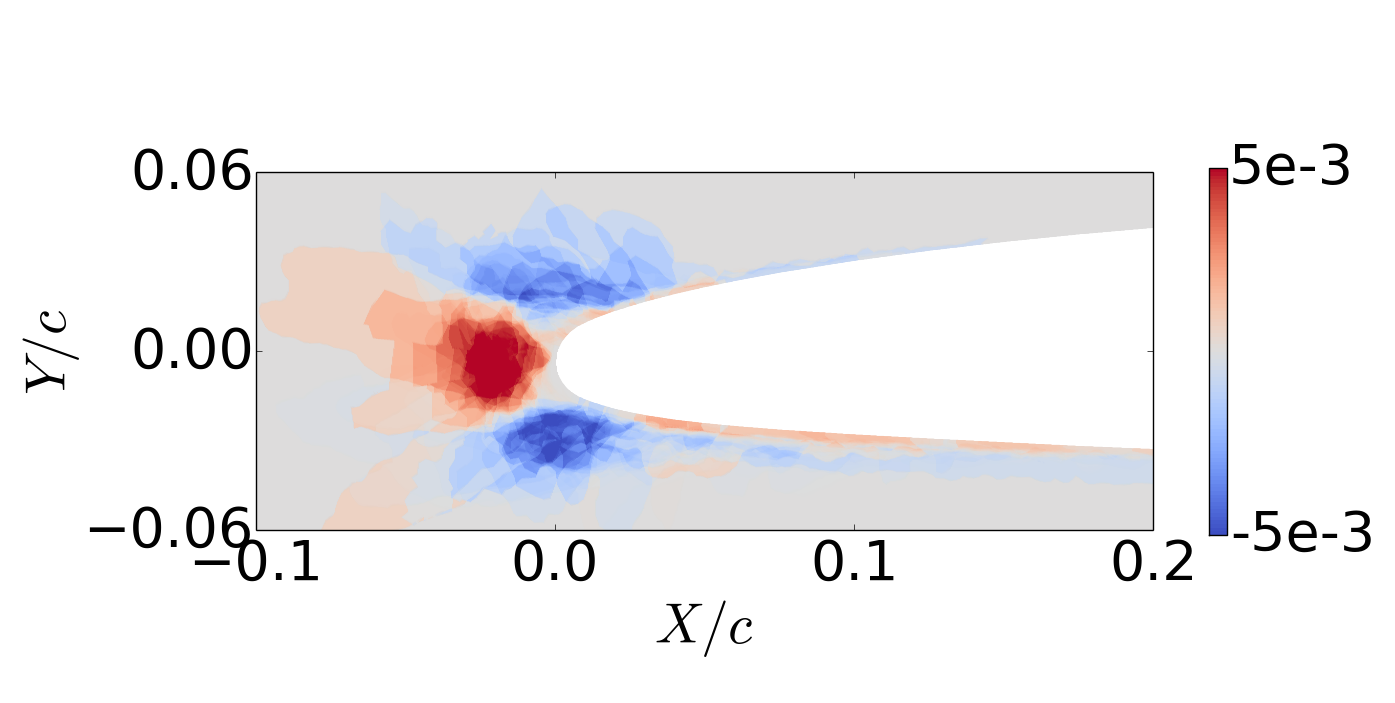
\includegraphics[width=0.4\textwidth]{MODE4}}
      \vspace*{1cm}\caption{Mean and POD modes.}
\end{figure}

\begin{itemize}
\item Represent ice shapes as composite sum of these pictures
\item Modes 1 and 2 simply add ice mass
\item Modes 3 and 4 switch between upper/lower surface horns and rime
\item Higher order modes contain more extreme shape perturbations
\end{itemize}
\end{frame}
\begin{frame}
\frametitle{POD Reconstructions}
\label{sec-2-6}

\begin{figure}
      \vspace*{-0.5cm}\subfigure{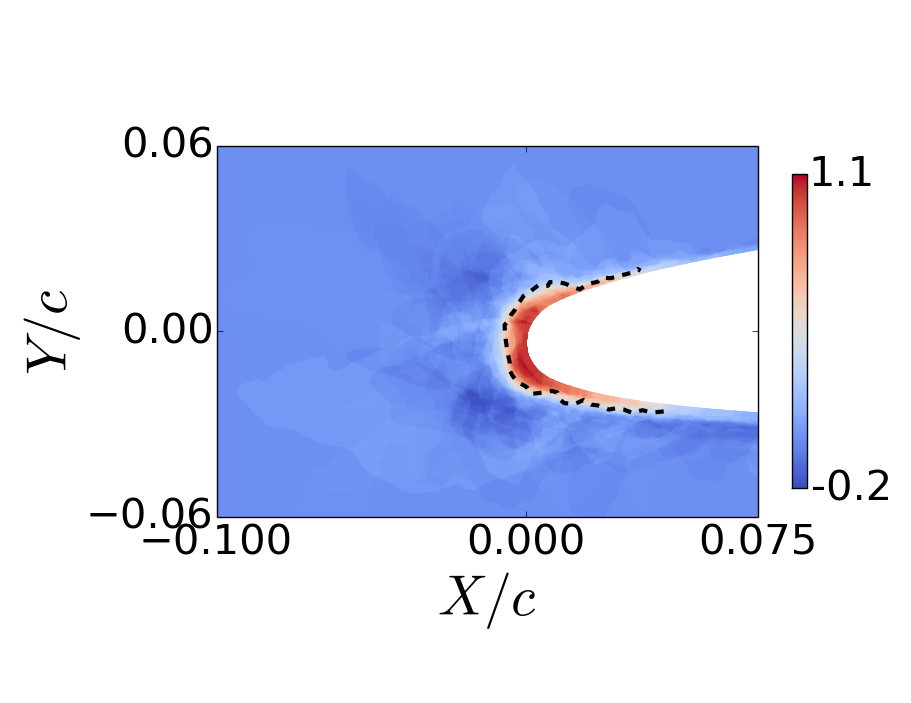
\includegraphics[width=0.3\textwidth]{UnfilteredReconstructionEx2.png}}
      \vspace*{-0.5cm}\subfigure{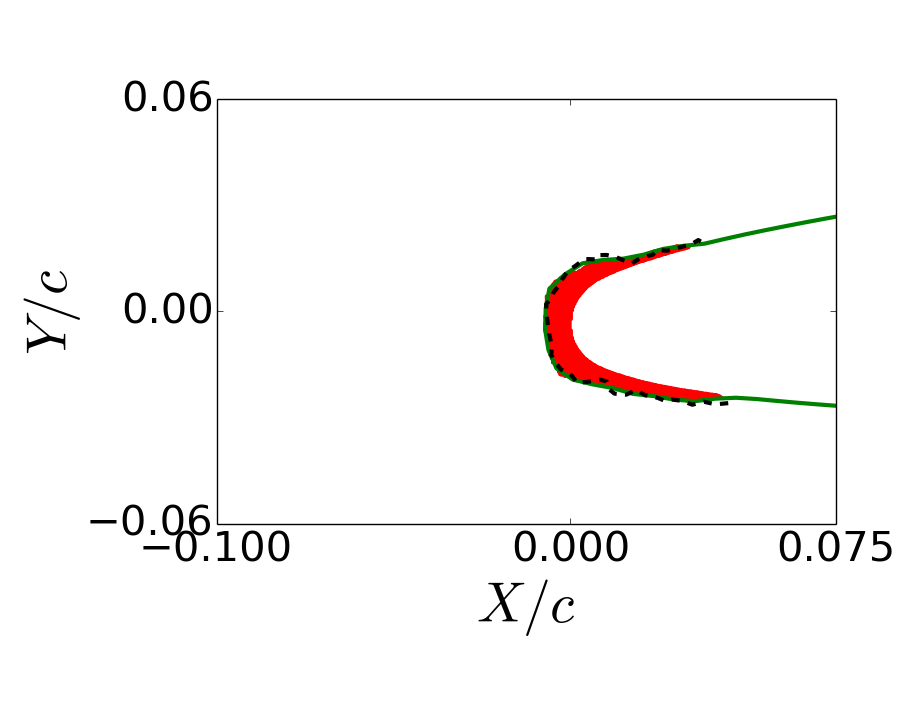
\includegraphics[width=0.3\textwidth]{FilteredReconstructionEx2.png}} \\
      \vspace*{-0.5cm}\subfigure{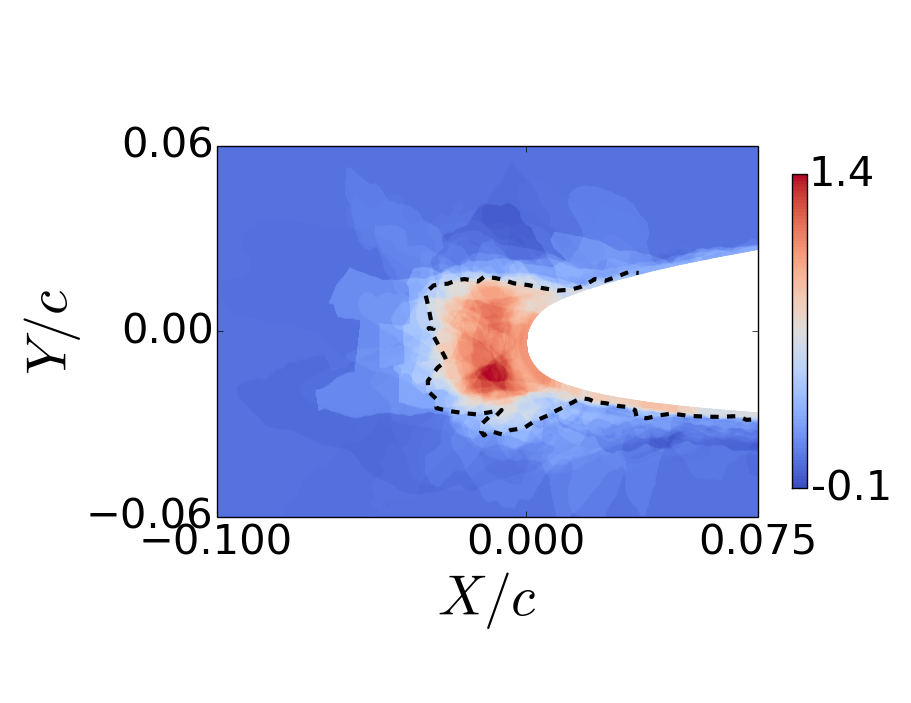
\includegraphics[width=0.3\textwidth]{UnfilteredReconstructionEx3.png}}
      \vspace*{-0.5cm}\subfigure{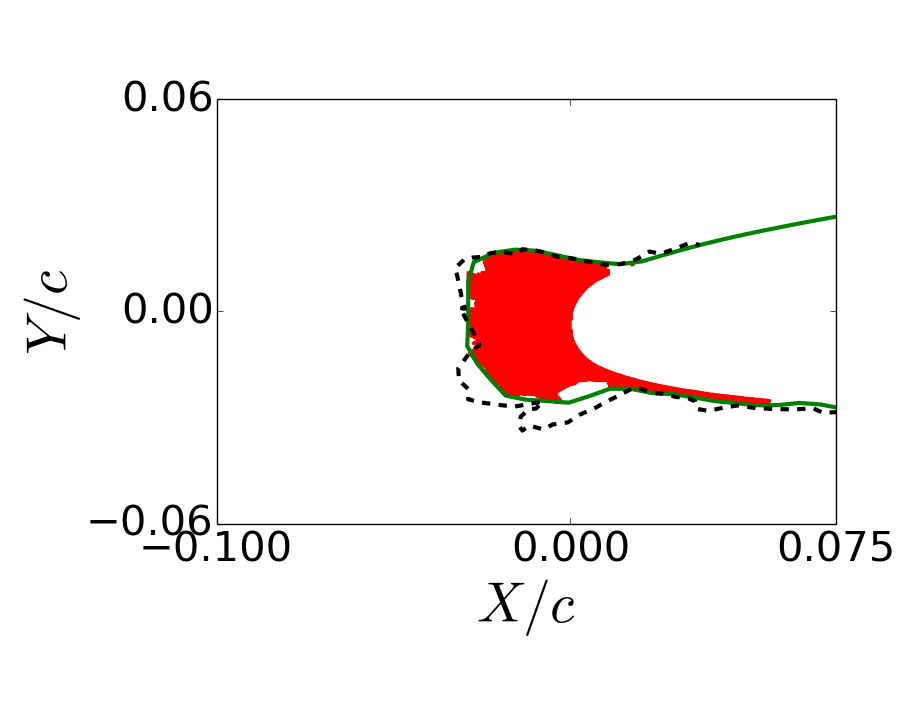
\includegraphics[width=0.3\textwidth]{FilteredReconstructionEx3.png}} \\
      \vspace*{-0.5cm}\subfigure{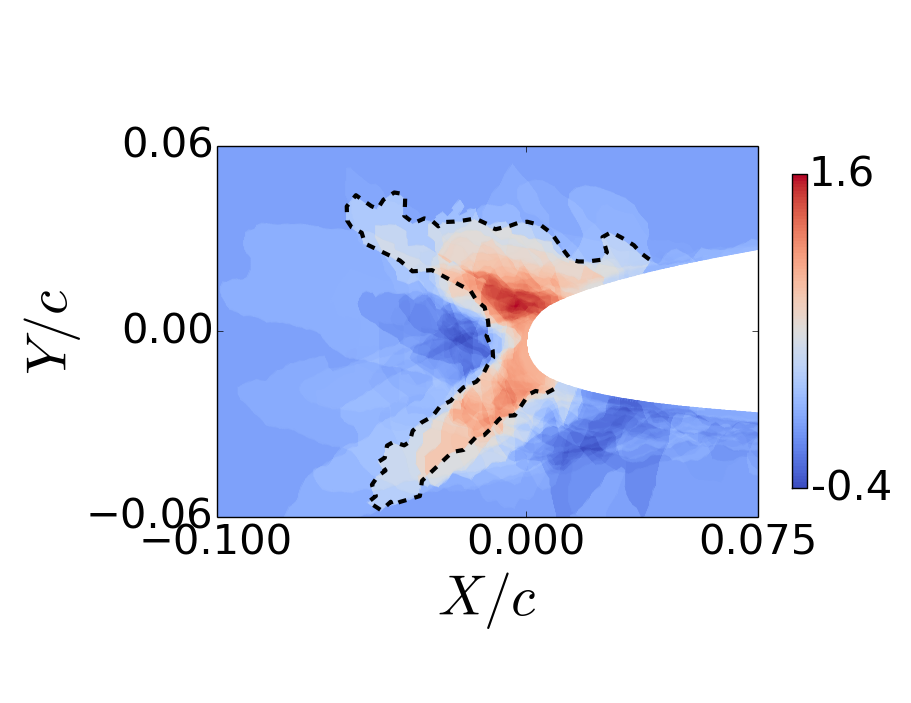
\includegraphics[width=0.3\textwidth]{UnfilteredReconstructionEx1.png}}
      \vspace*{-0.5cm}\subfigure{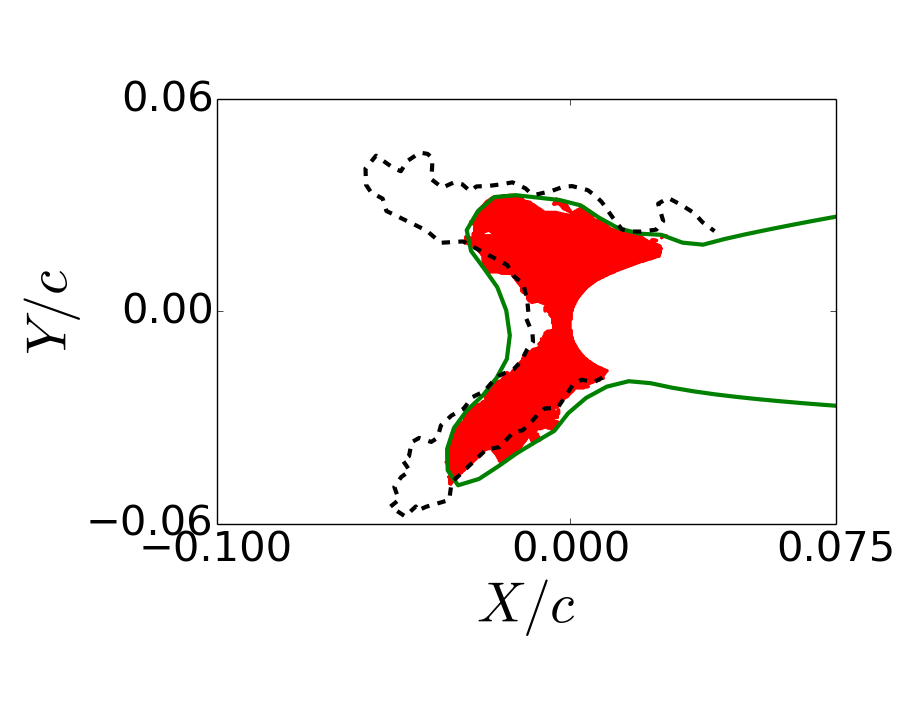
\includegraphics[width=0.3\textwidth]{FilteredReconstructionEx1.png}}
      \vspace*{0cm}\caption{POD reconstructions.}
\end{figure}

\begin{itemize}
\item Agreement is great for shapes close to mean, less good for extreme shapes
\end{itemize}
\end{frame}
\begin{frame}
\frametitle{Link Physical Conditions to Modes}
\label{sec-2-7}

\vspace*{-0.5cm}\begin{figure}
      \vspace*{-0.4cm}\subfigure{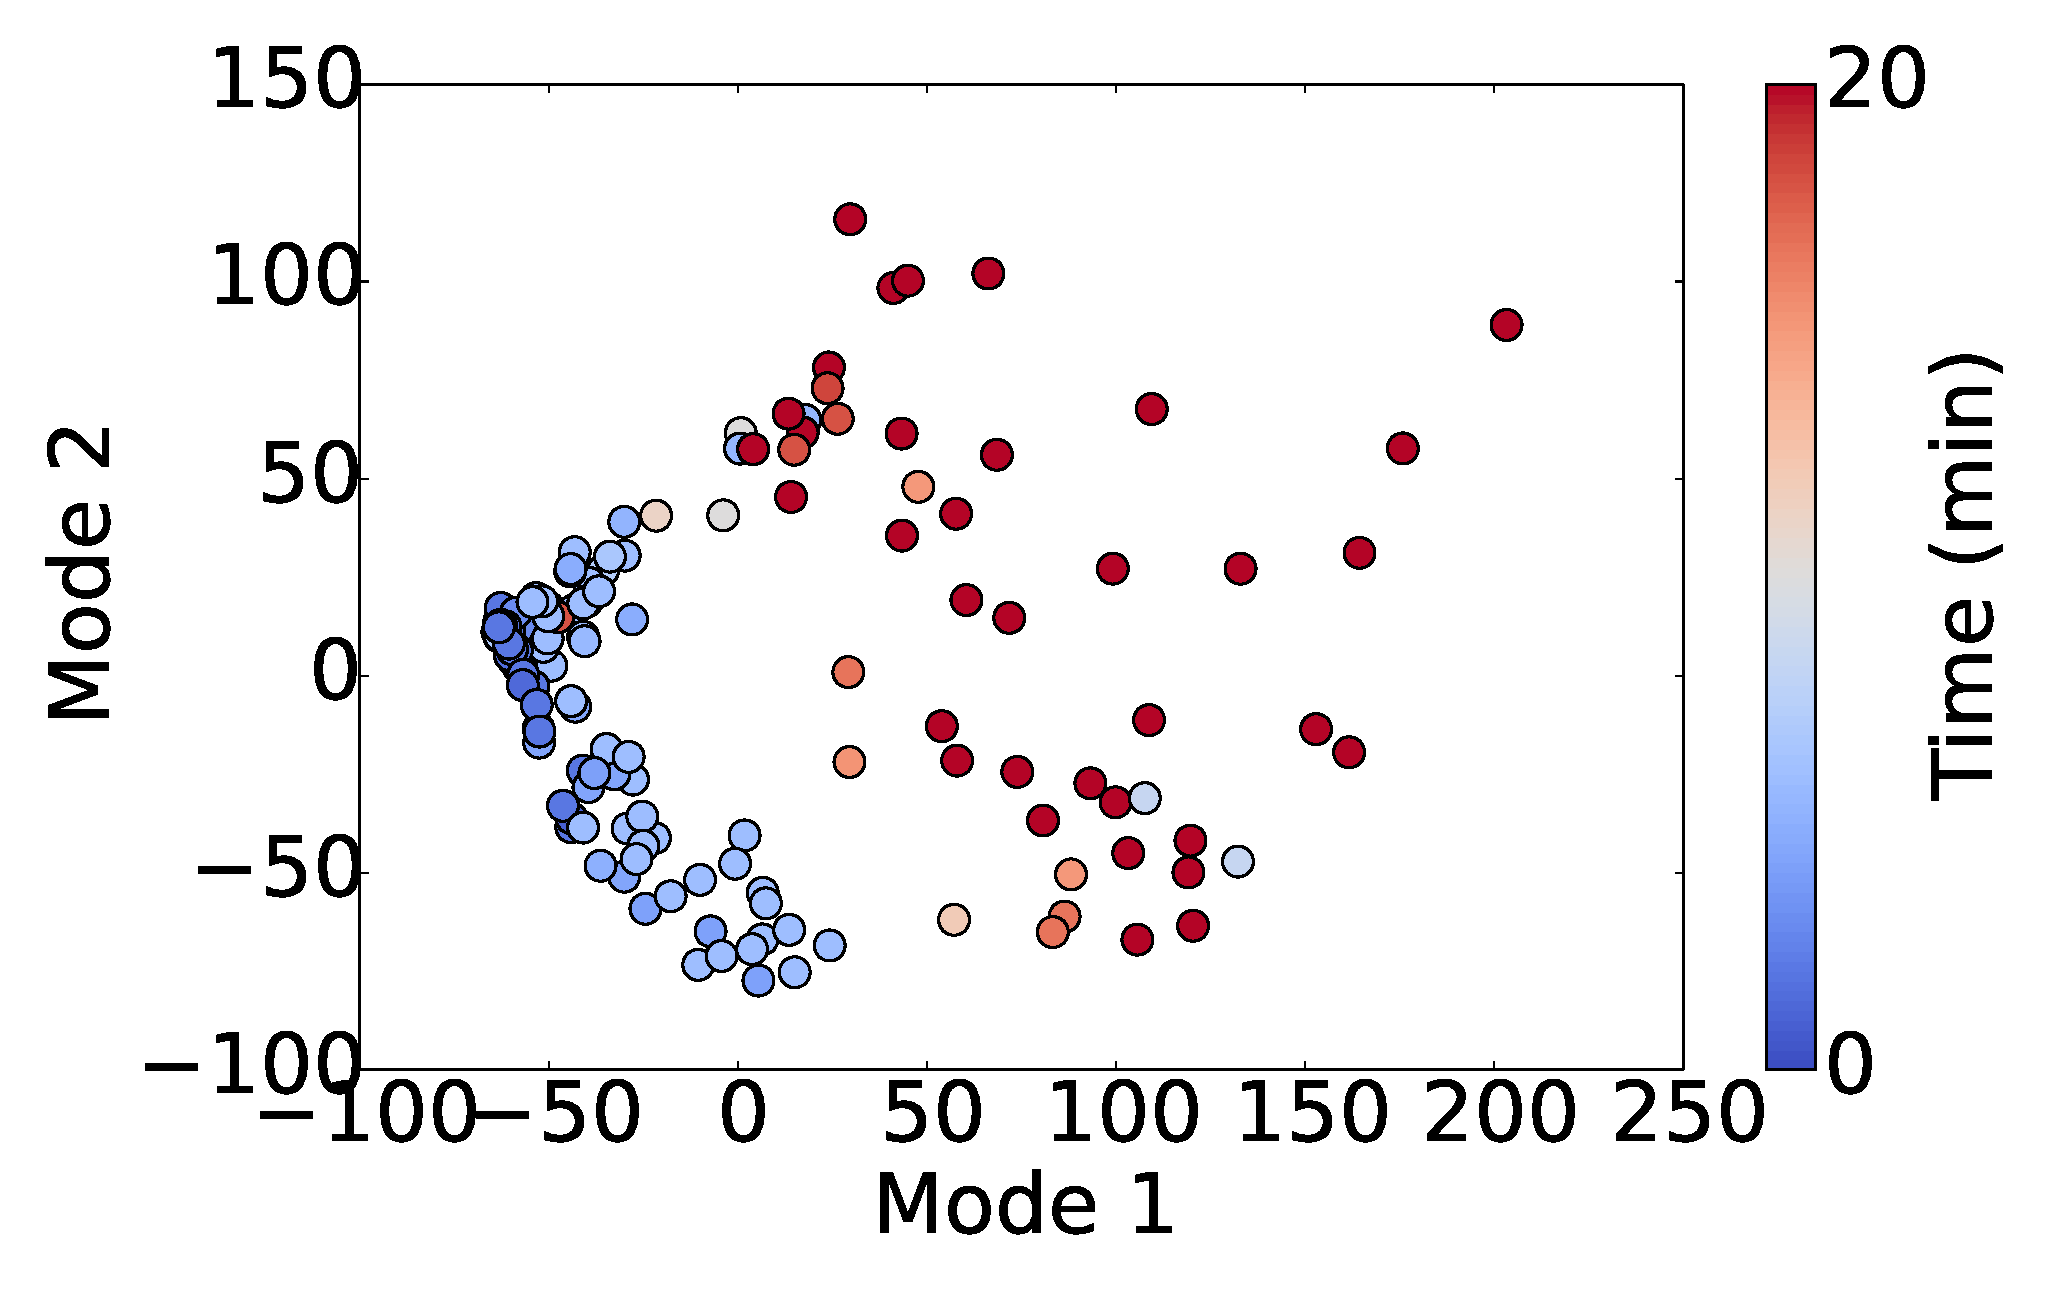
\includegraphics[width=0.35\textwidth]{10ParamMode1Mode2Time}}
      \vspace*{-0.4cm}\subfigure{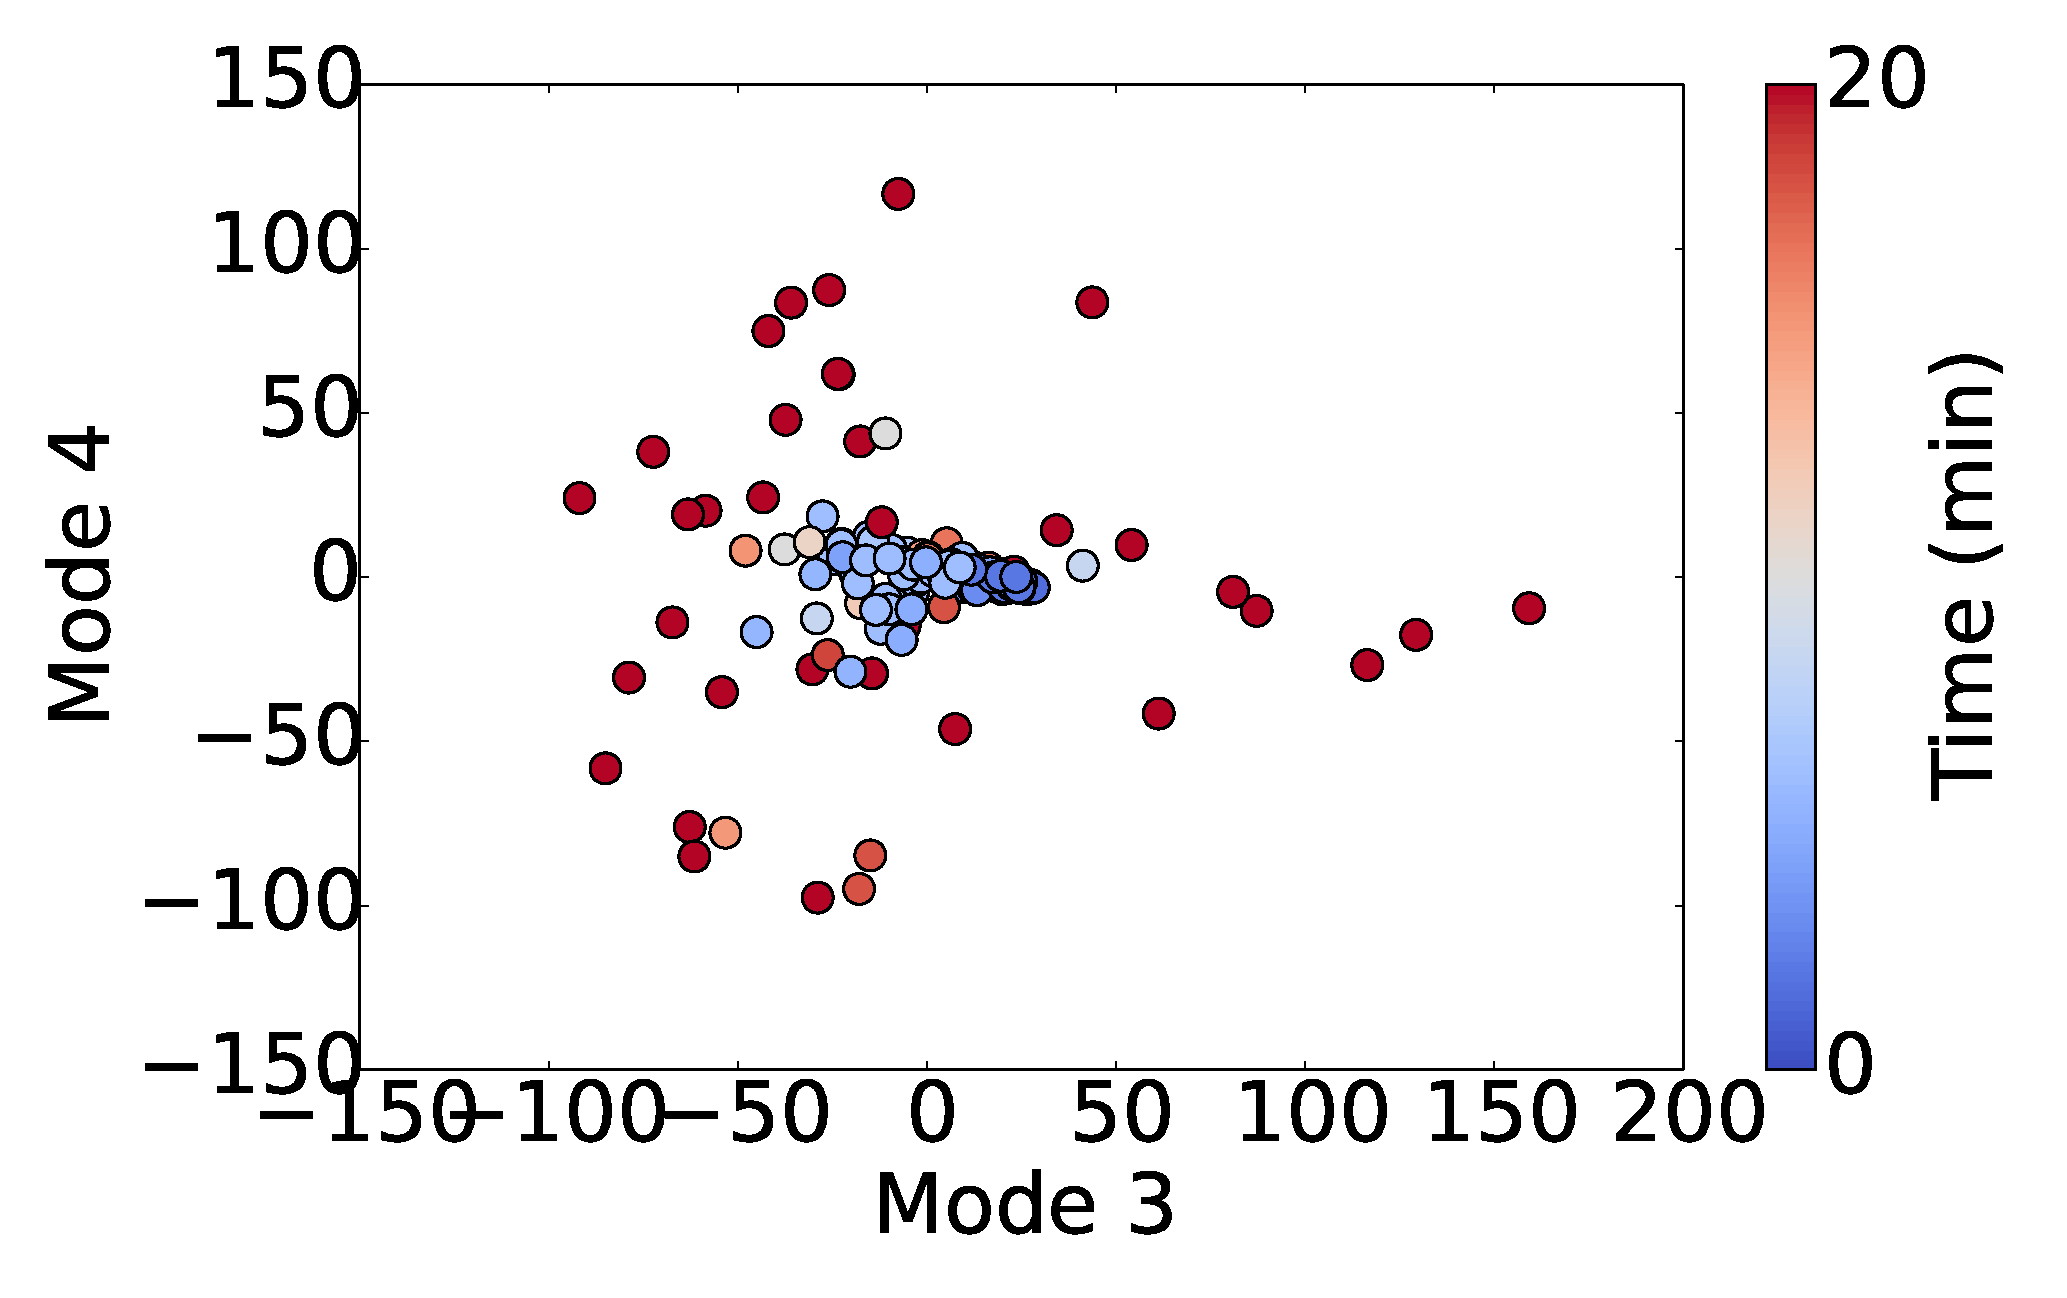
\includegraphics[width=0.35\textwidth]{10ParamMode3Mode4Time}} \\
      \vspace*{-0.35cm}\subfigure{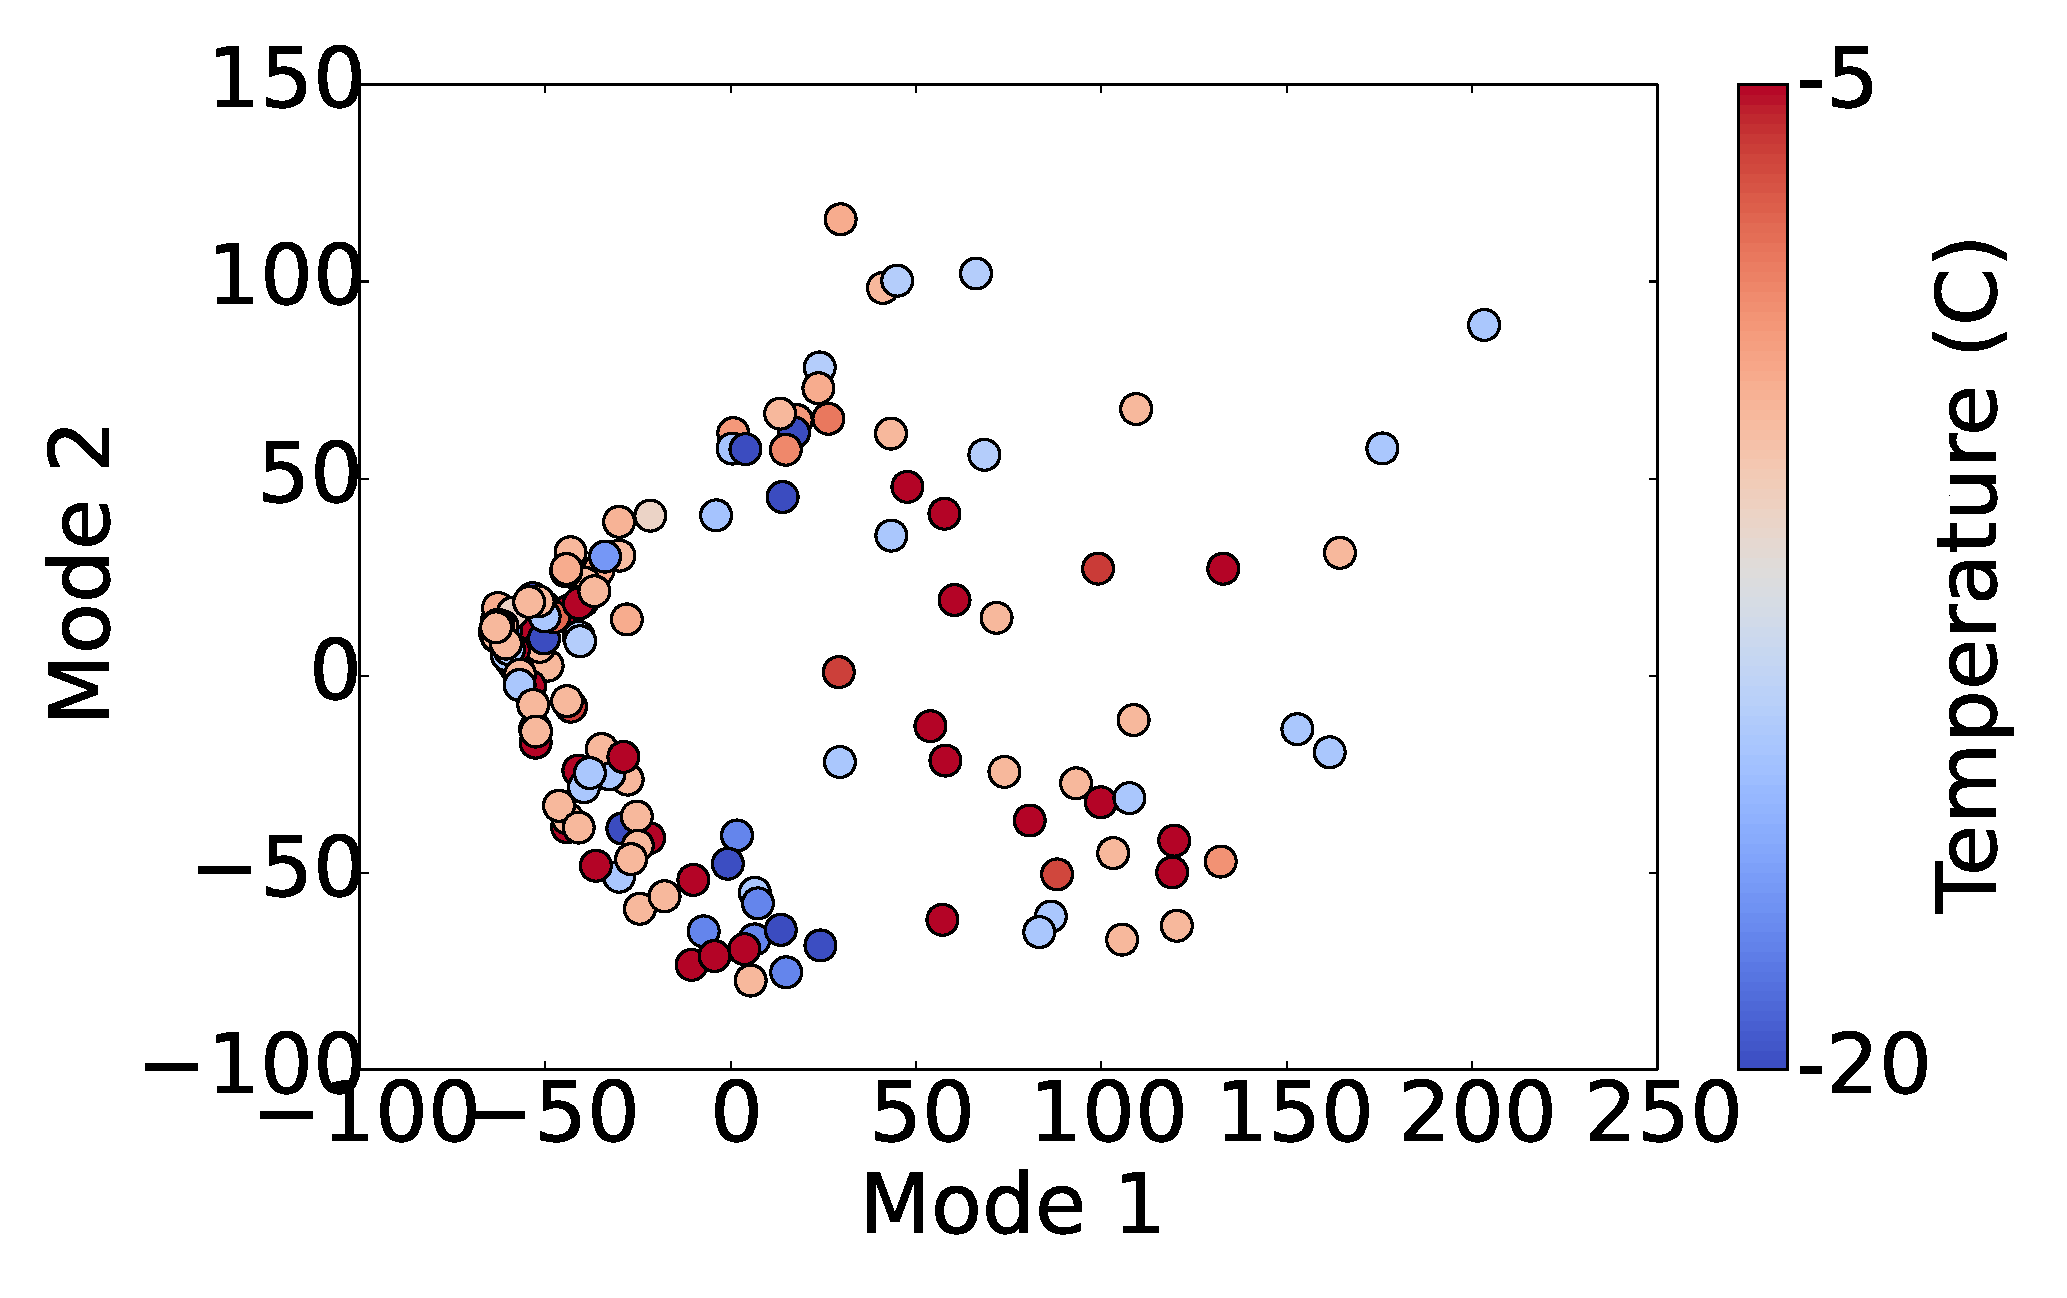
\includegraphics[width=0.35\textwidth]{10ParamMode1Mode2Temp}}
      \vspace*{-0.35cm}\subfigure{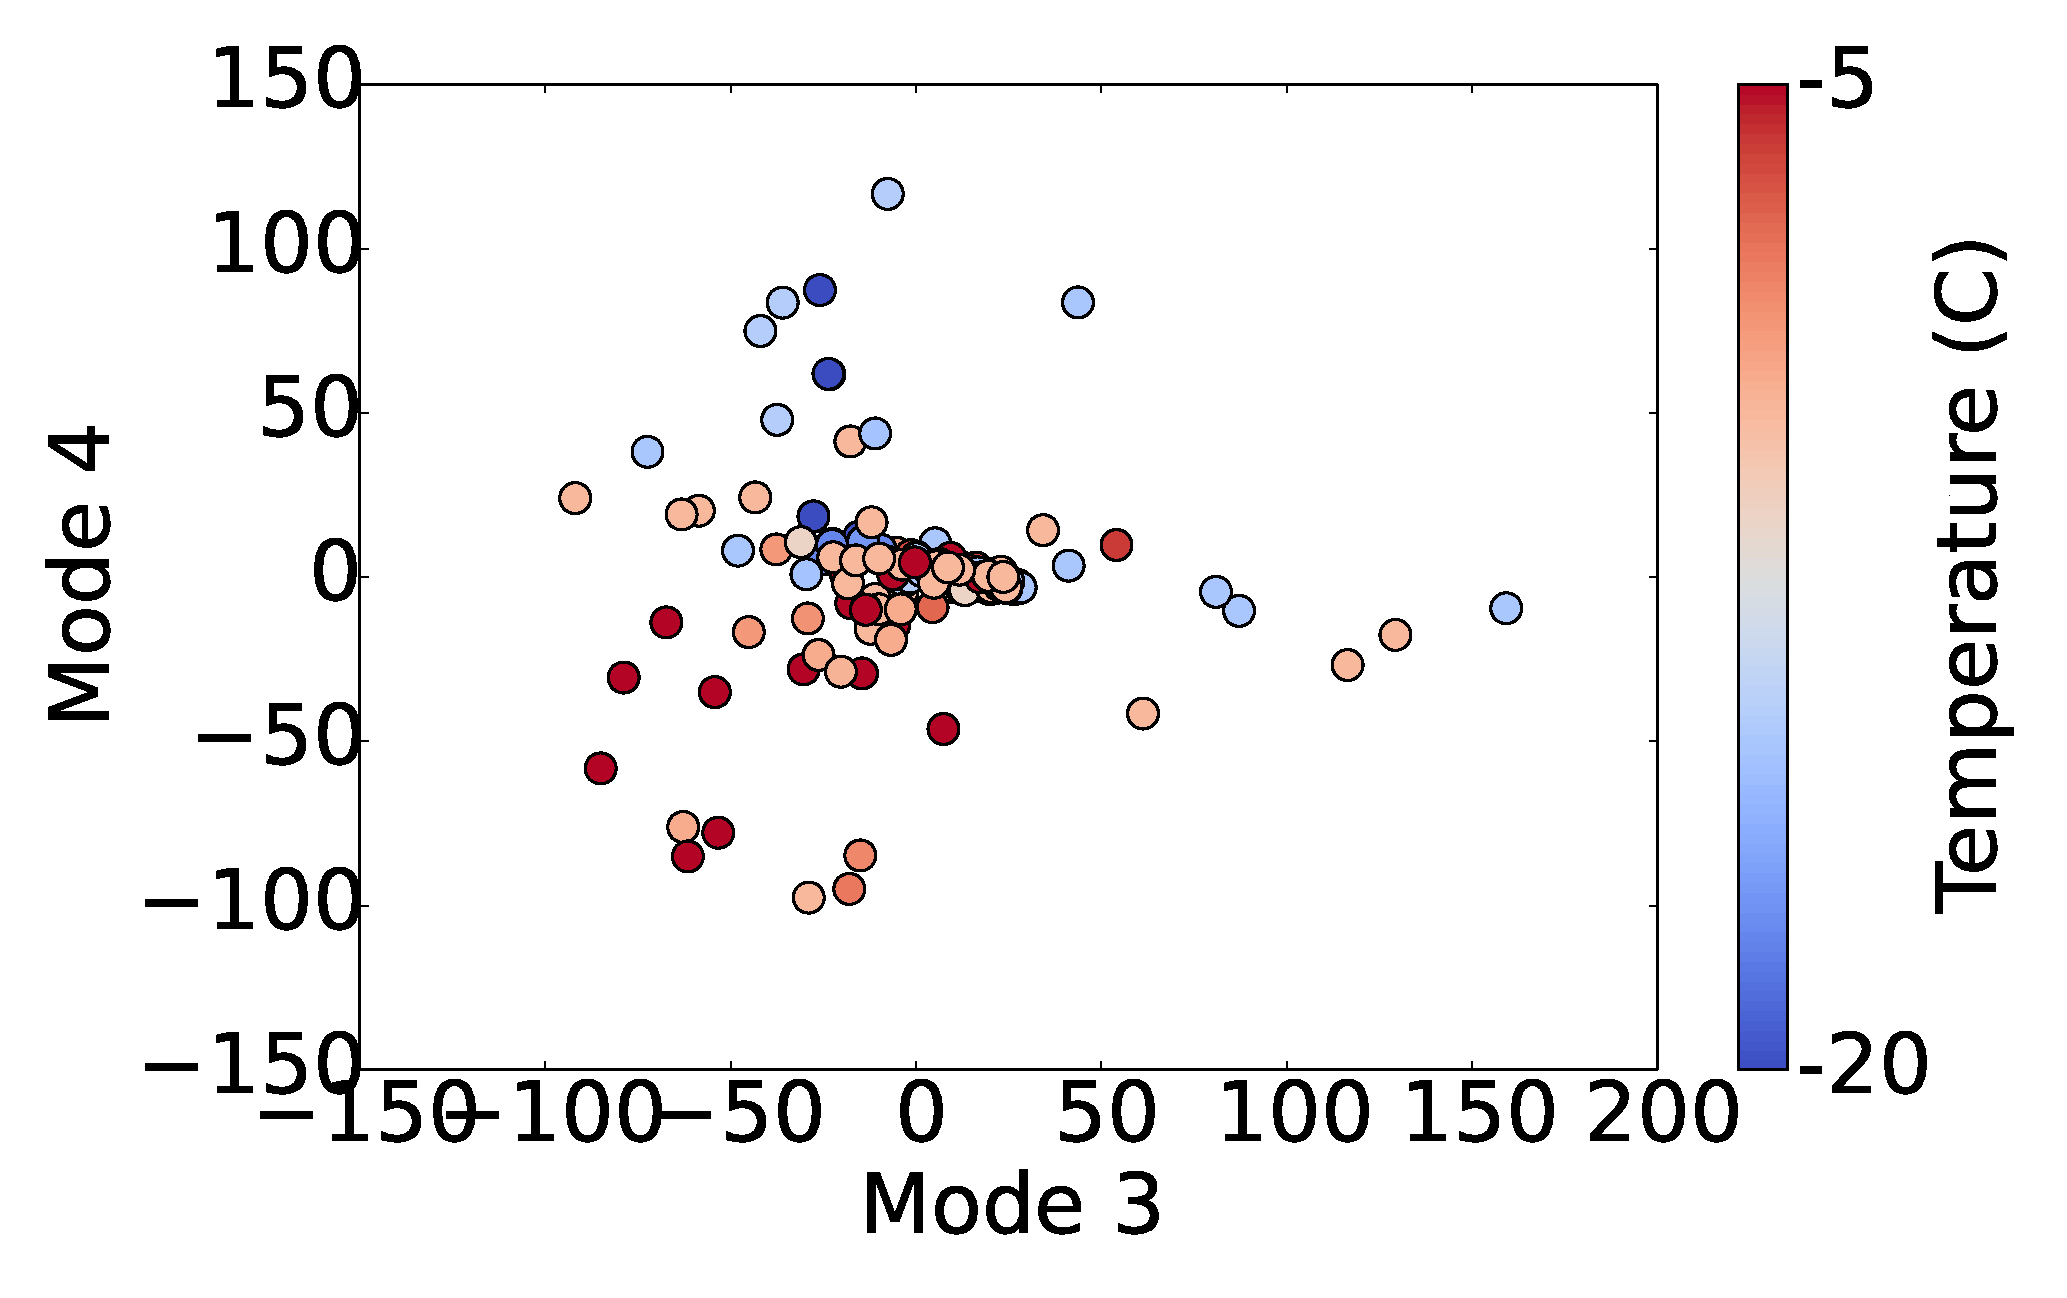
\includegraphics[width=0.35\textwidth]{10ParamMode3Mode4Temp}} \\
      \vspace*{-0.35cm}\subfigure{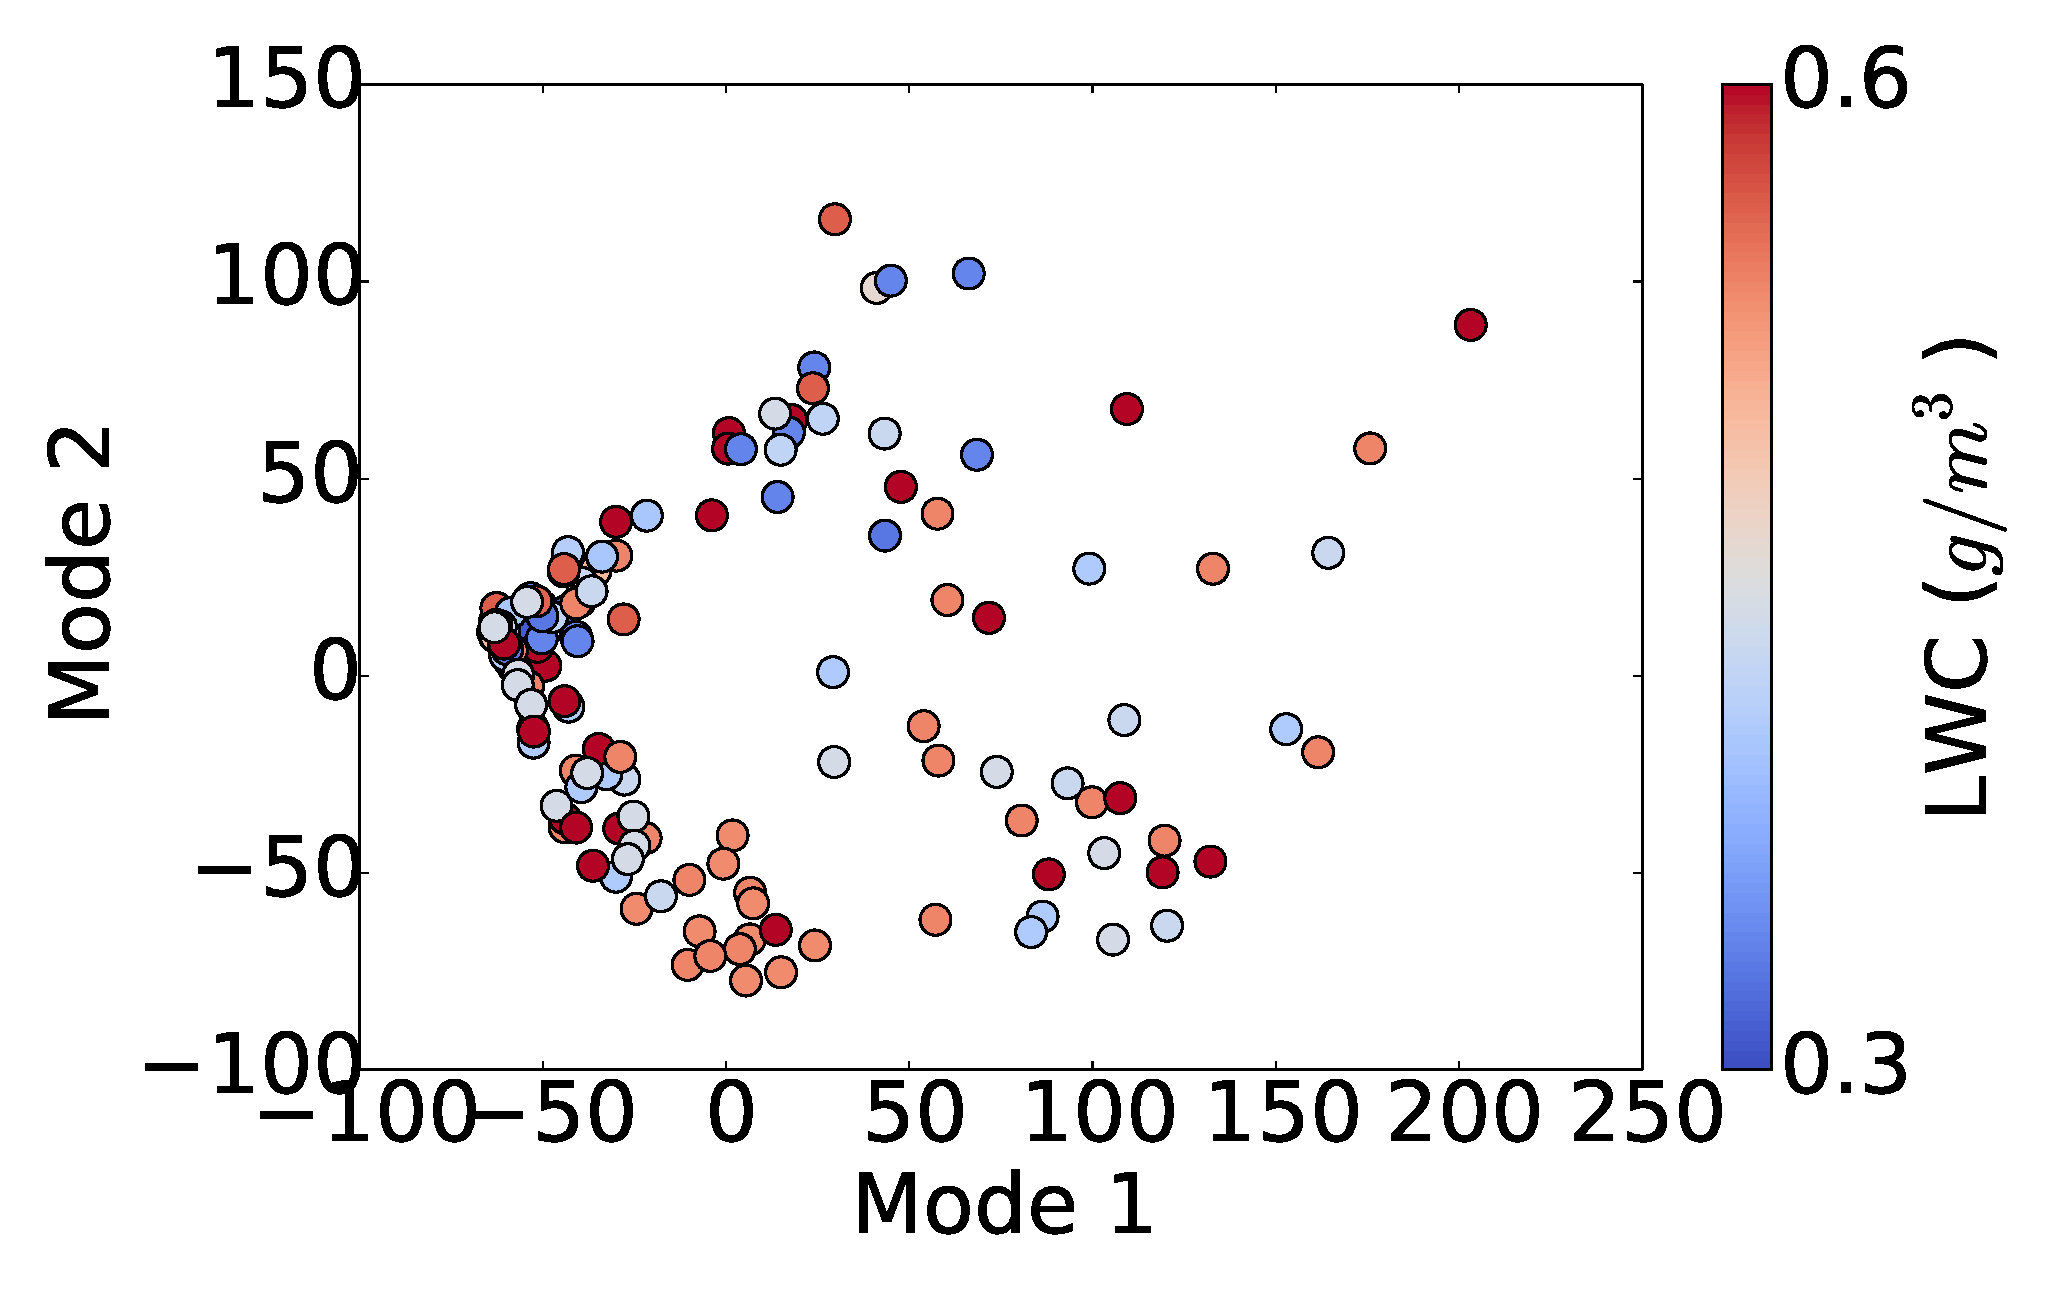
\includegraphics[width=0.35\textwidth]{10ParamMode1Mode2LWC}}
      \vspace*{-0.35cm}\subfigure{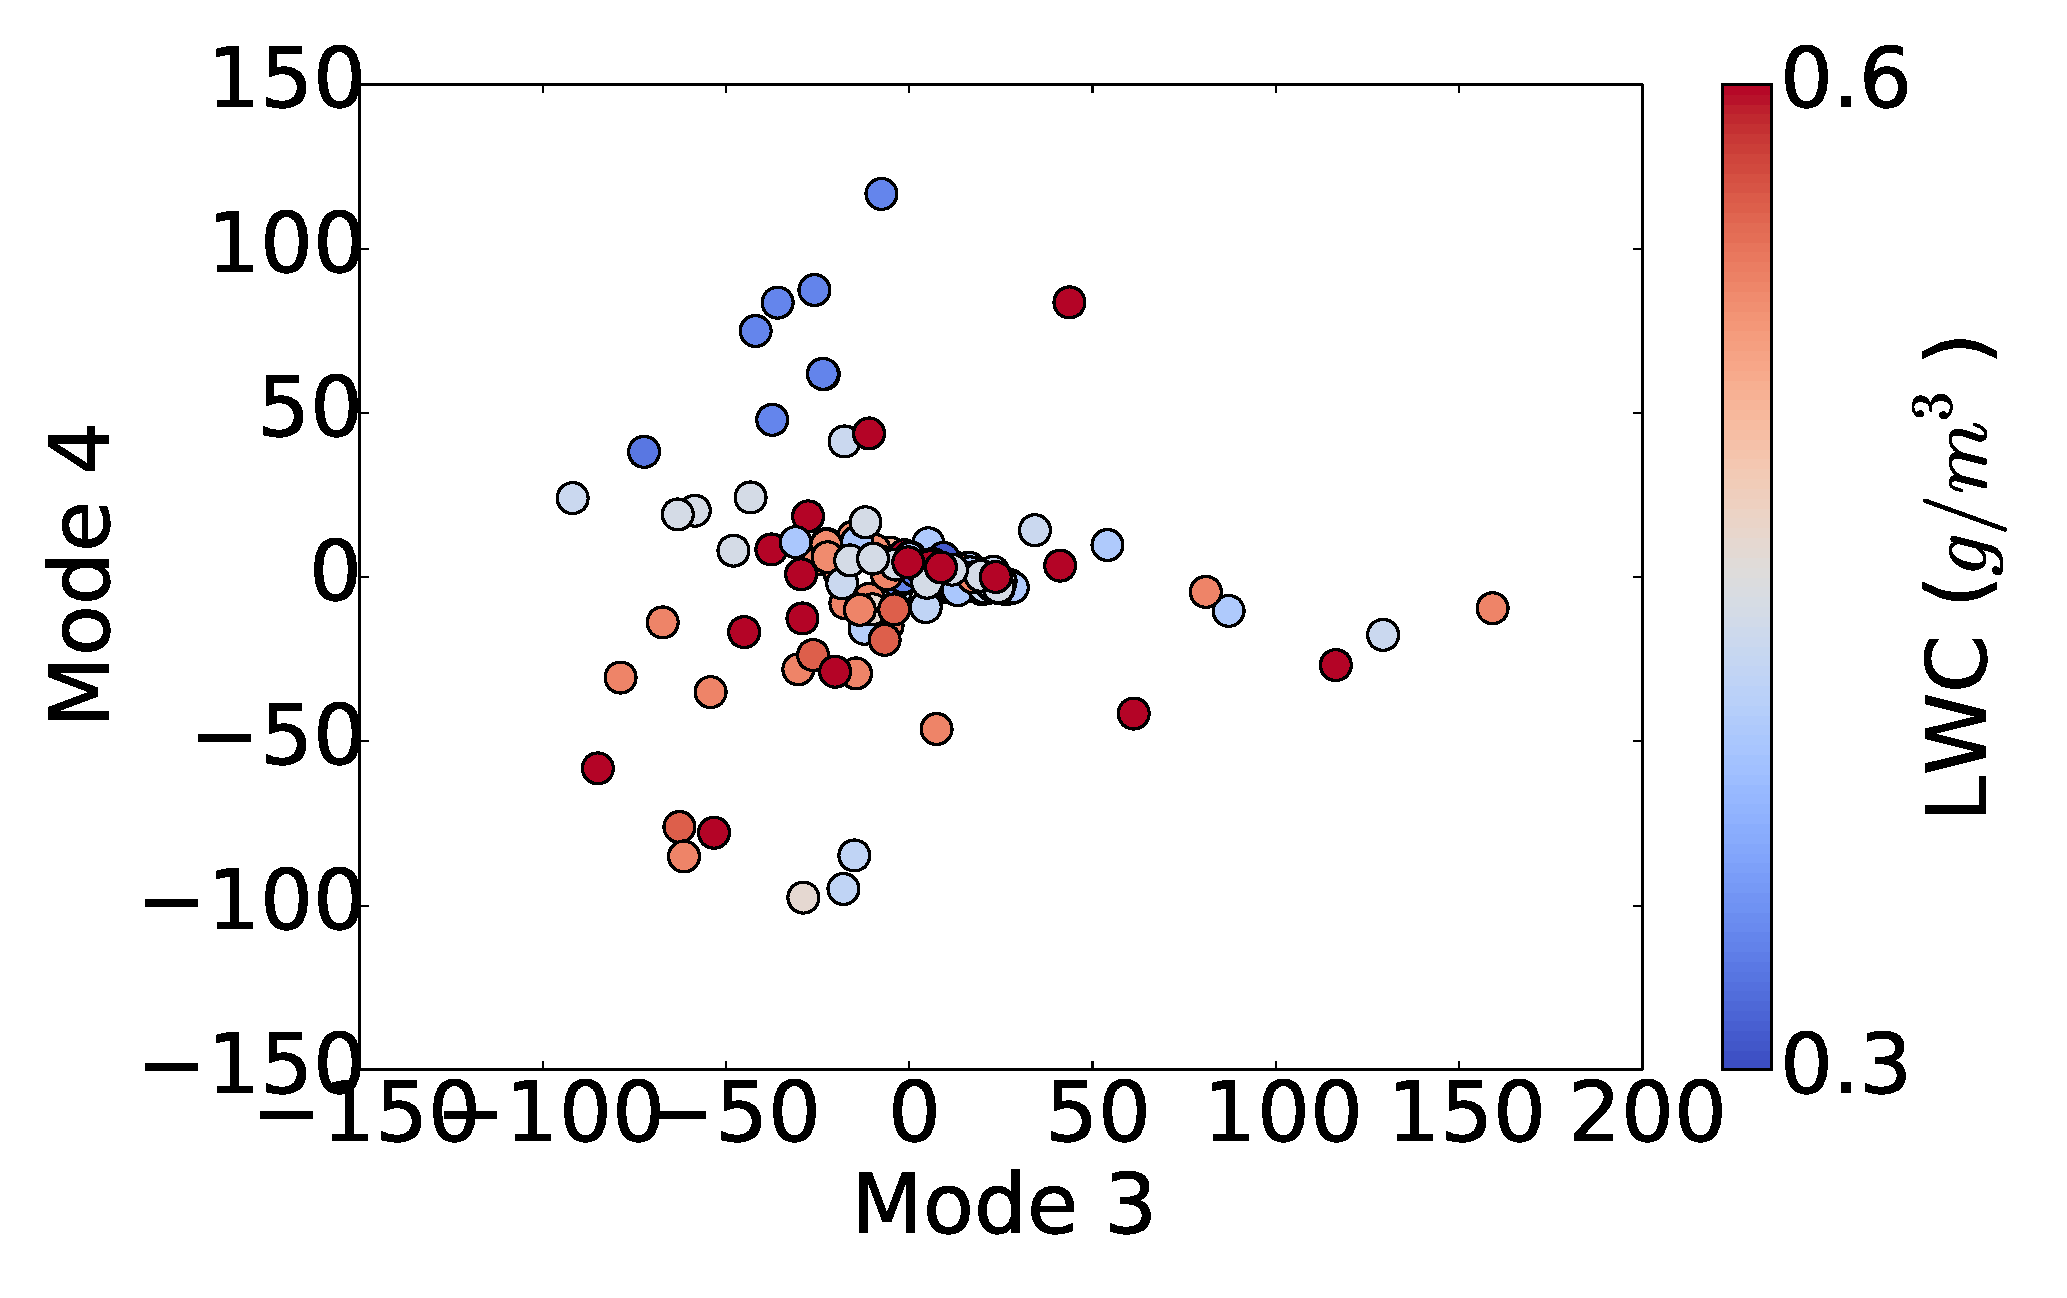
\includegraphics[width=0.35\textwidth]{10ParamMode3Mode4LWC}}
      \vspace*{0cm}\caption{POD coefficients, colored with parameters.}
\end{figure}

\begin{itemize}
\item Statistically relate time, temperature and LWC to POD modes
\item Input conditions, output POD coefficients that respect the data
\end{itemize}
\end{frame}
\begin{frame}
\frametitle{Data-Driven Icing Model}
\label{sec-2-8}

\fontsize{7}\selectfont
% Define the layers to draw the diagram
\pgfdeclarelayer{background}
\pgfdeclarelayer{foreground}
\pgfsetlayers{background,main,foreground}

\begin{figure}[!ht]
  % Define block styles used later
  \tikzstyle{sensor}=[draw, fill=blue!20, text width=5em, 
    text centered, minimum height=2.5em]
  \tikzstyle{ann} = [above, text width=10em, text centered]
  \tikzstyle{wa} = [sensor, text width=8em, fill=blue!20, 
    minimum height=3em, rounded corners]
  % Define distances for bordering
  %\def\blockdist{2.3}
  %\def\edgedist{2.5}
  \vspace*{-1cm}
  \begin{tikzpicture}

    \begin{pgfonlayer}{background}
      \path (1.5,1) node (b) {};
      \path (7.5,-1) node (c) {};
      \path[fill=orange!40,rounded corners, draw=black!50, dashed] (b) rectangle (c);
    \end{pgfonlayer}

    \node (Input) [wa] {{\bf Input}\vspace*{4\em}\\-- Time\\-- Temperature\\-- LWC};
    \path (Input)+(3,0) node (Database) [wa] {{\bf Database}\vspace*{4\em}\\-- Ice shapes\\-- Conditions};
    \path (Database)+(3,0) node (Statistics) [wa] {{\bf Statistics}\vspace*{4\em}\\-- Filtered coeffs\\-- Random samples};
    \path (Statistics)+(3,0) node (Reconstruction) [wa] {{\bf Shape}\vspace*{4\em}\\$\bv{X} = \sum_i^{M} c_i \phi_i$};

    \path [draw, ->, thick] (Input.east) |- node [above] {} (Database.west);
    \path [draw, ->, thick] (Database.east) -- node [below] {} (Statistics.west);
    \path [draw, ->, thick] (Statistics.east) -- node [below] {} (Reconstruction.west);

  \end{tikzpicture}
  \caption{Flowchart of data-driven model.}
\end{figure}
\fontsize{9}\selectfont
\begin{itemize}
\item Input physical condition ranges
\item Filter database for shapes that match conditions
\item Create POD coefficient distributions for downselected data
\item Generate random samples from these distributions
\item Reconstruct ice shape using data-inferred POD coefficients
\end{itemize}
\end{frame}
\begin{frame}
\frametitle{Random Shapes}
\label{sec-2-9}

\begin{figure}
      \vspace*{-0.4cm}\subfigure{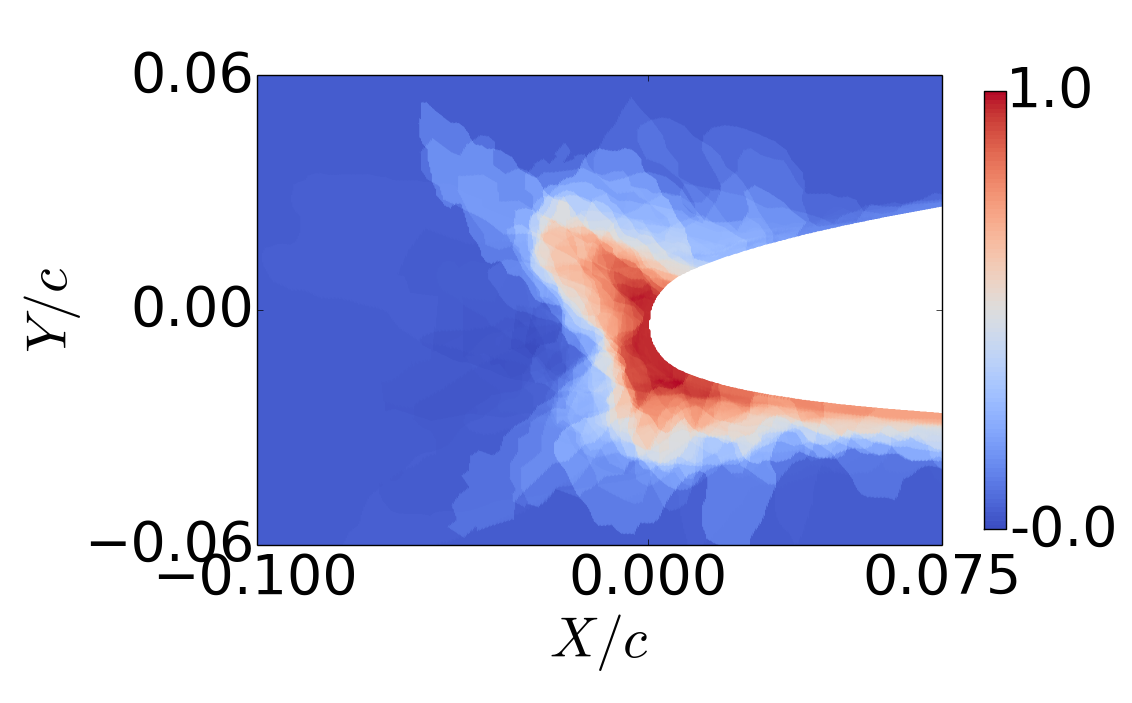
\includegraphics[width=0.4\textwidth]{10ParamHornFromPhysics}}
      \vspace*{-0.4cm}\subfigure{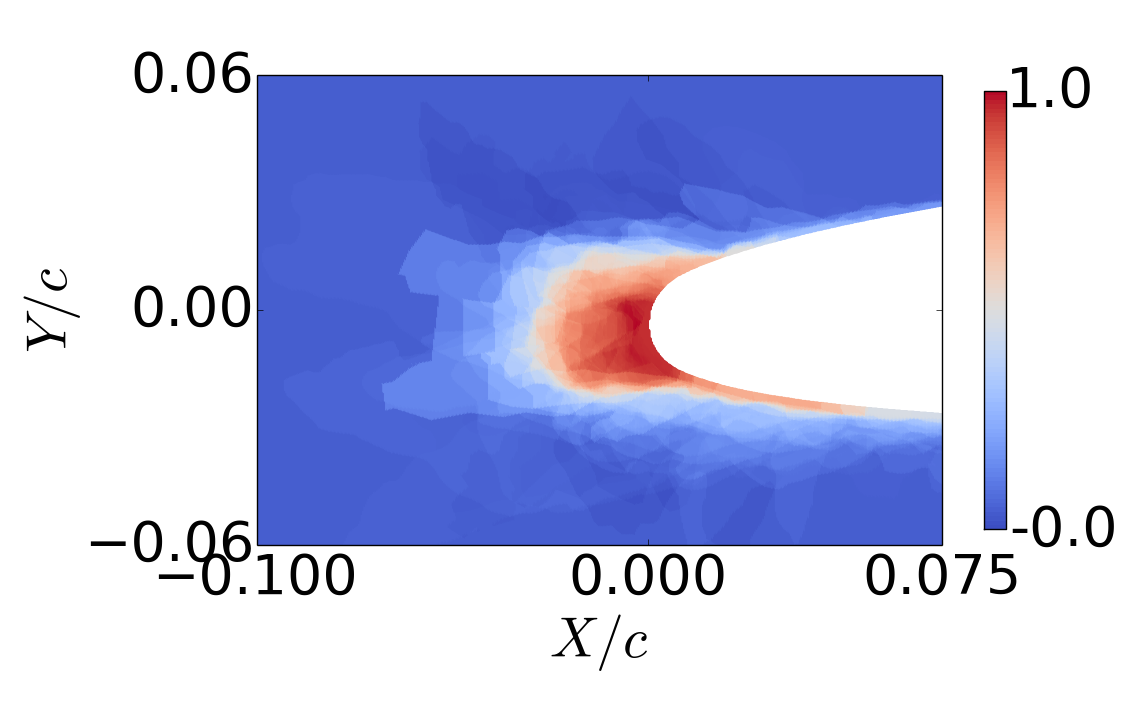
\includegraphics[width=0.4\textwidth]{10ParamRimeFromPhysics}} \\
      \vspace*{-0.4cm}\subfigure[Time > 10 min; temperature > -10 C; LWC > 0.45 $g/m^3$]{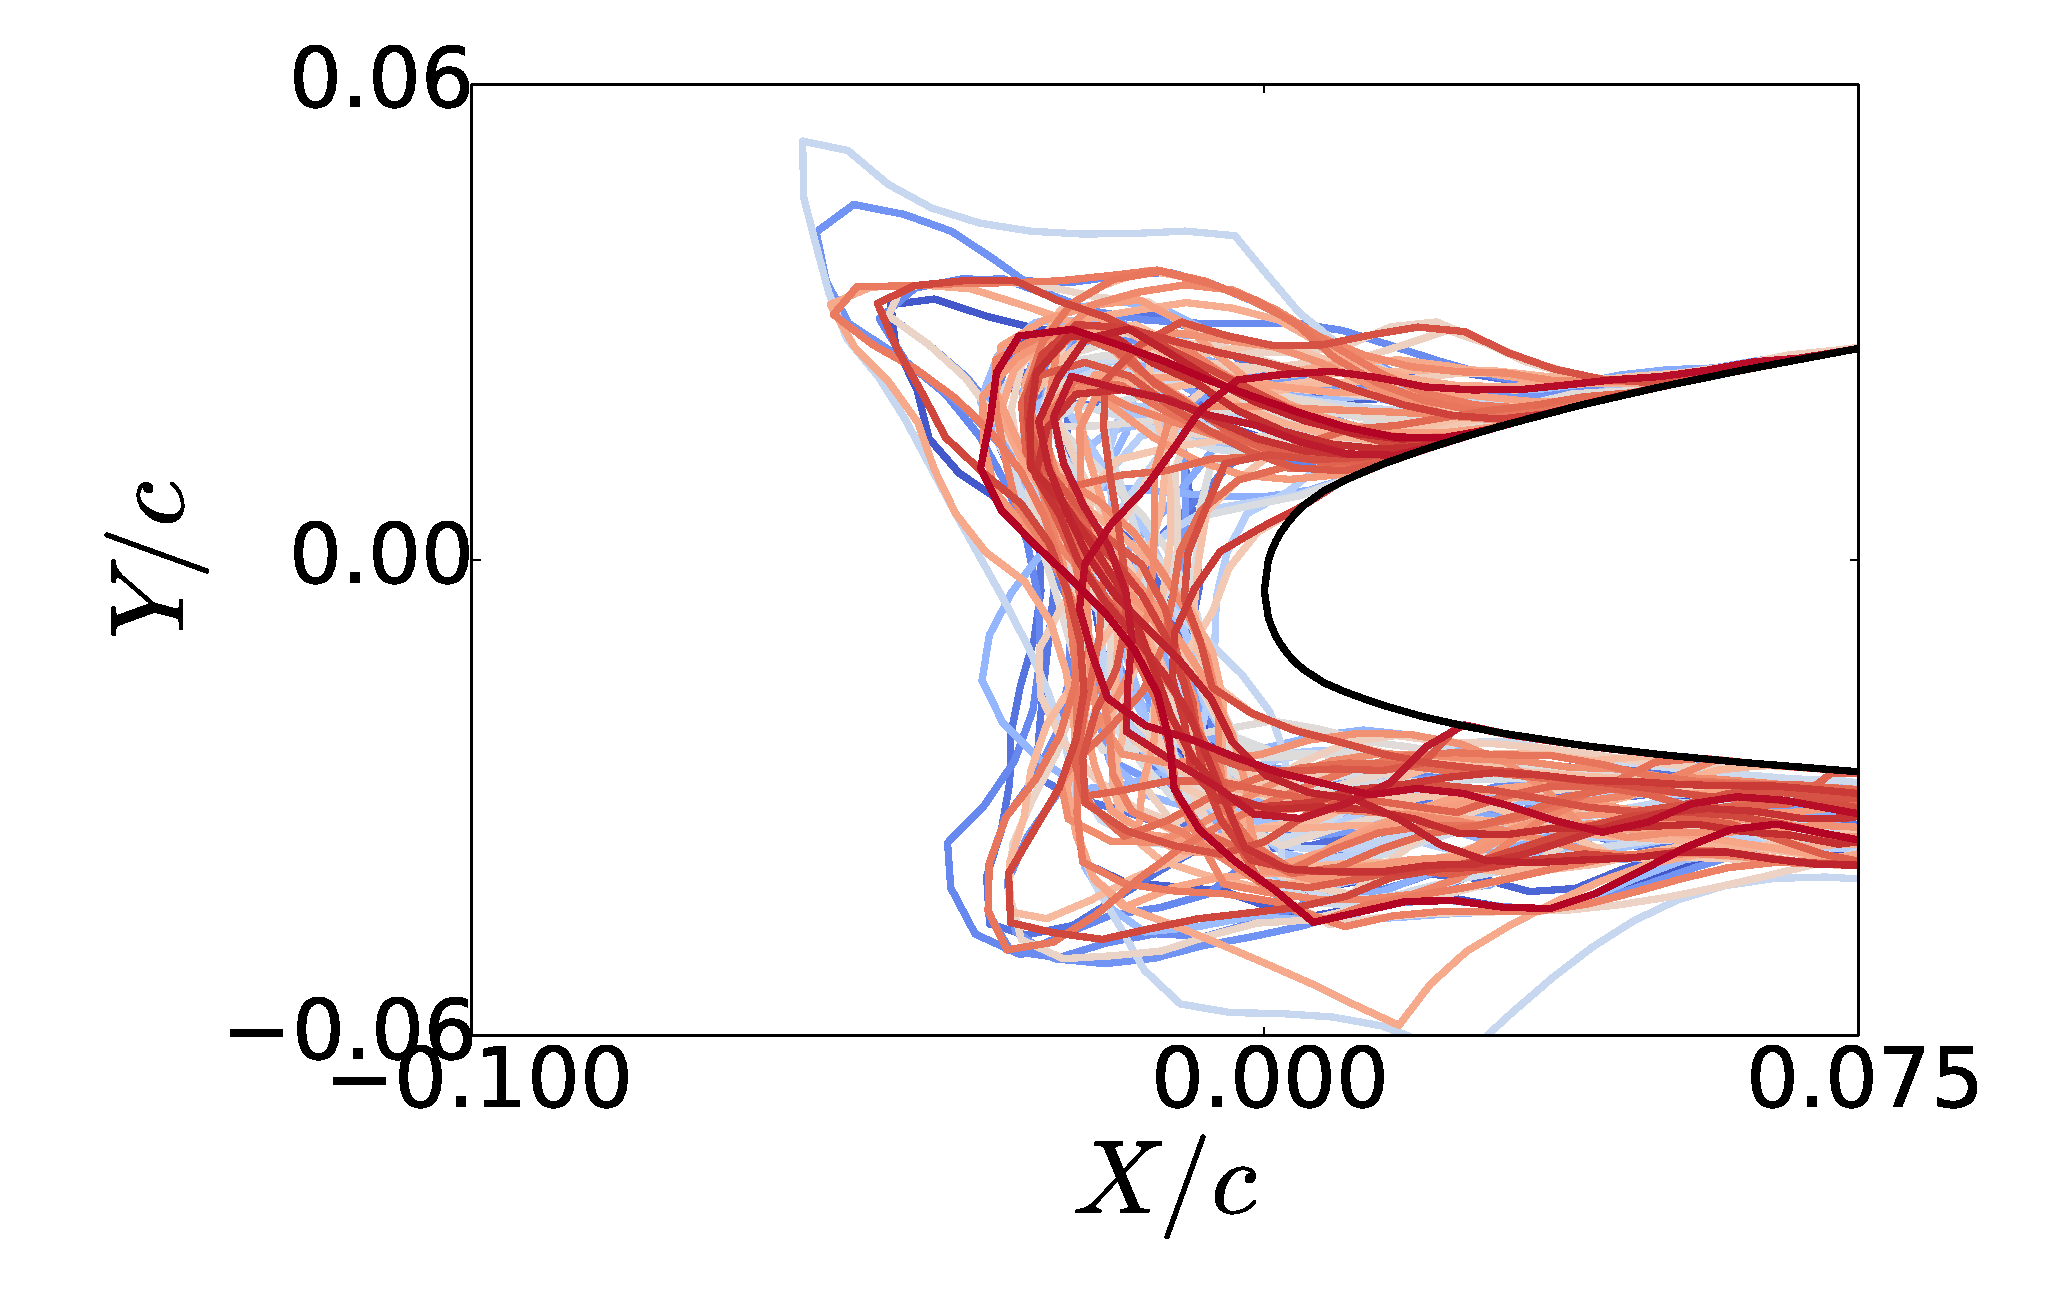
\includegraphics[width=0.4\textwidth]{10ParamRandomHorns}}
      \vspace*{-0.4cm}\subfigure[Time > 10 min; temperature < -10 C; LWC < 0.45 $g/m^3$]{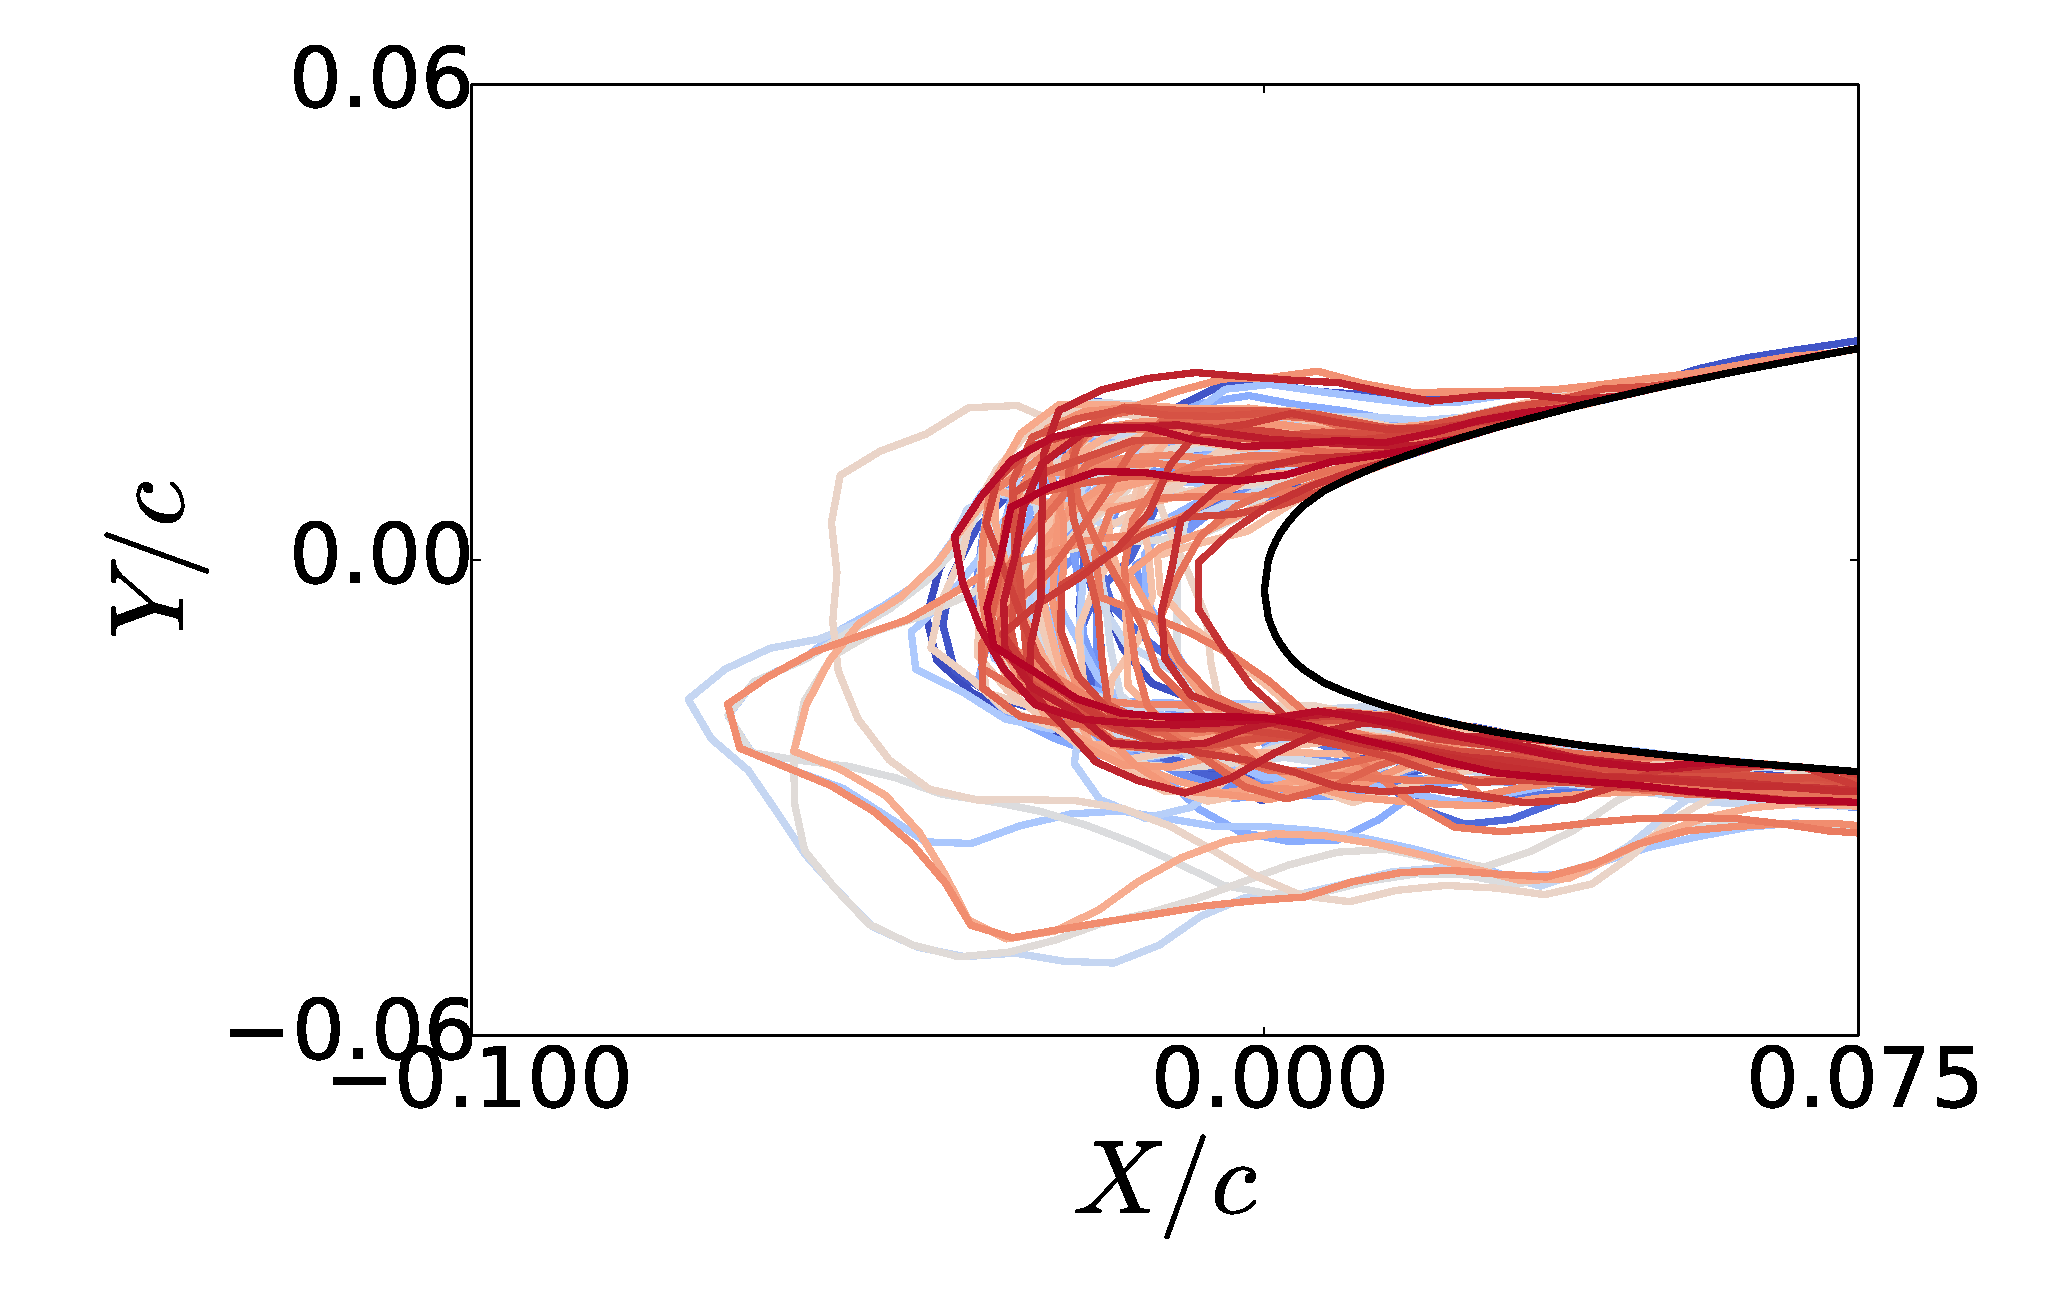
\includegraphics[width=0.4\textwidth]{10ParamRandomRime}}
      \vspace*{0cm}\caption{Random data-driven ice shapes.}
\end{figure}

\begin{itemize}
\item These shapes were generated at random, no physics
\end{itemize}
\end{frame}
\begin{frame}
\frametitle{Uncertainty Quantification}
\label{sec-2-10}

\vspace*{-0.0cm}\begin{figure}
      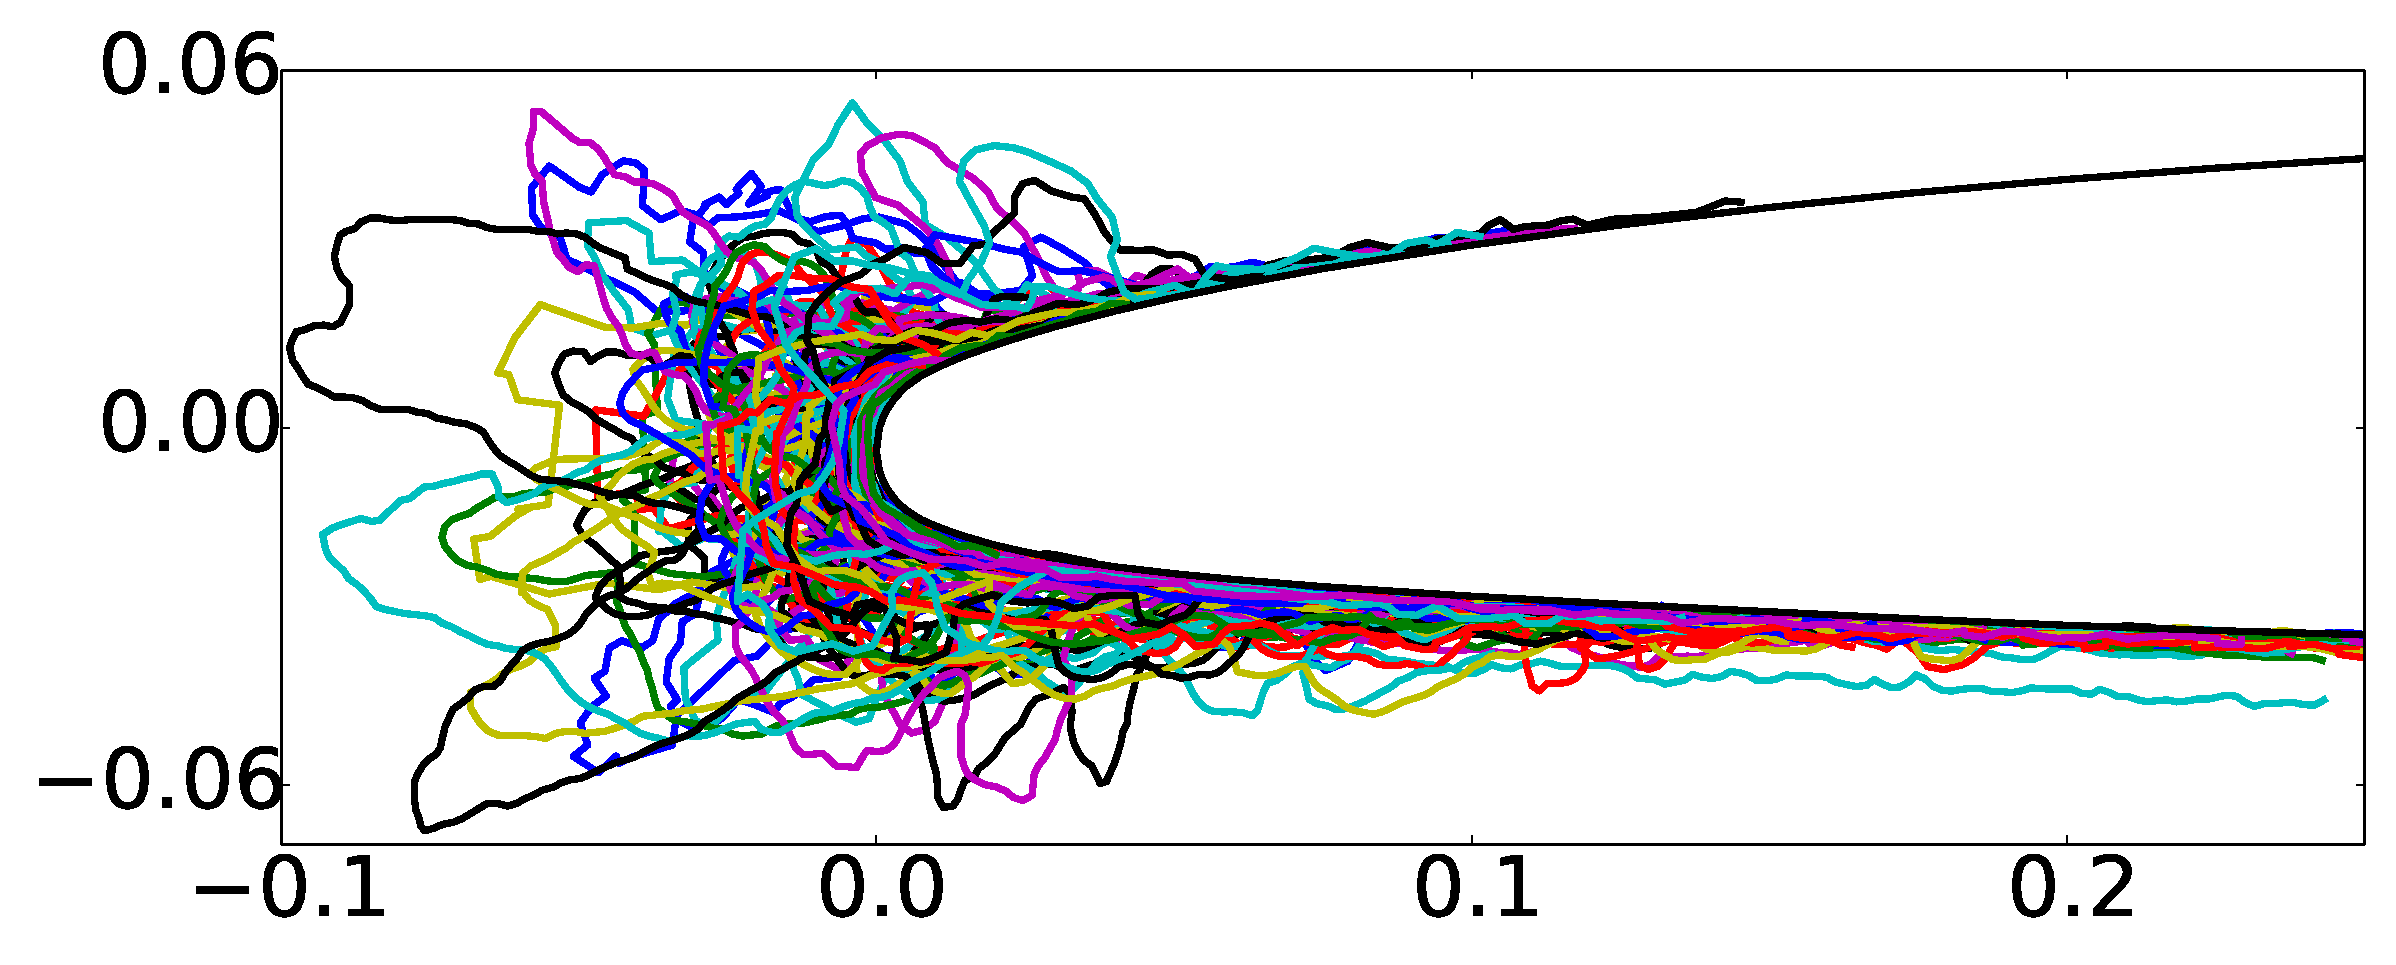
\includegraphics[width=0.5\textwidth]{GlobalDataSet}
      \caption{Wind tunnel experimental ice shapes}
\end{figure}
\textbf{Goal:} Quantify performance variation with POD modes

\textbf{Approach:}
\begin{itemize}
\item Generate random samples in POD space with Latin Hypercube Sampling (LHS)
\item Test corresponding shapes with flow solver
\item Quantify lift/drag statistics
\end{itemize}
\end{frame}
\begin{frame}
\frametitle{Latin Hypercube Samples}
\label{sec-2-11}

\vspace*{-0.0cm}\begin{figure}
      \vspace*{-1.5cm}\subfigure{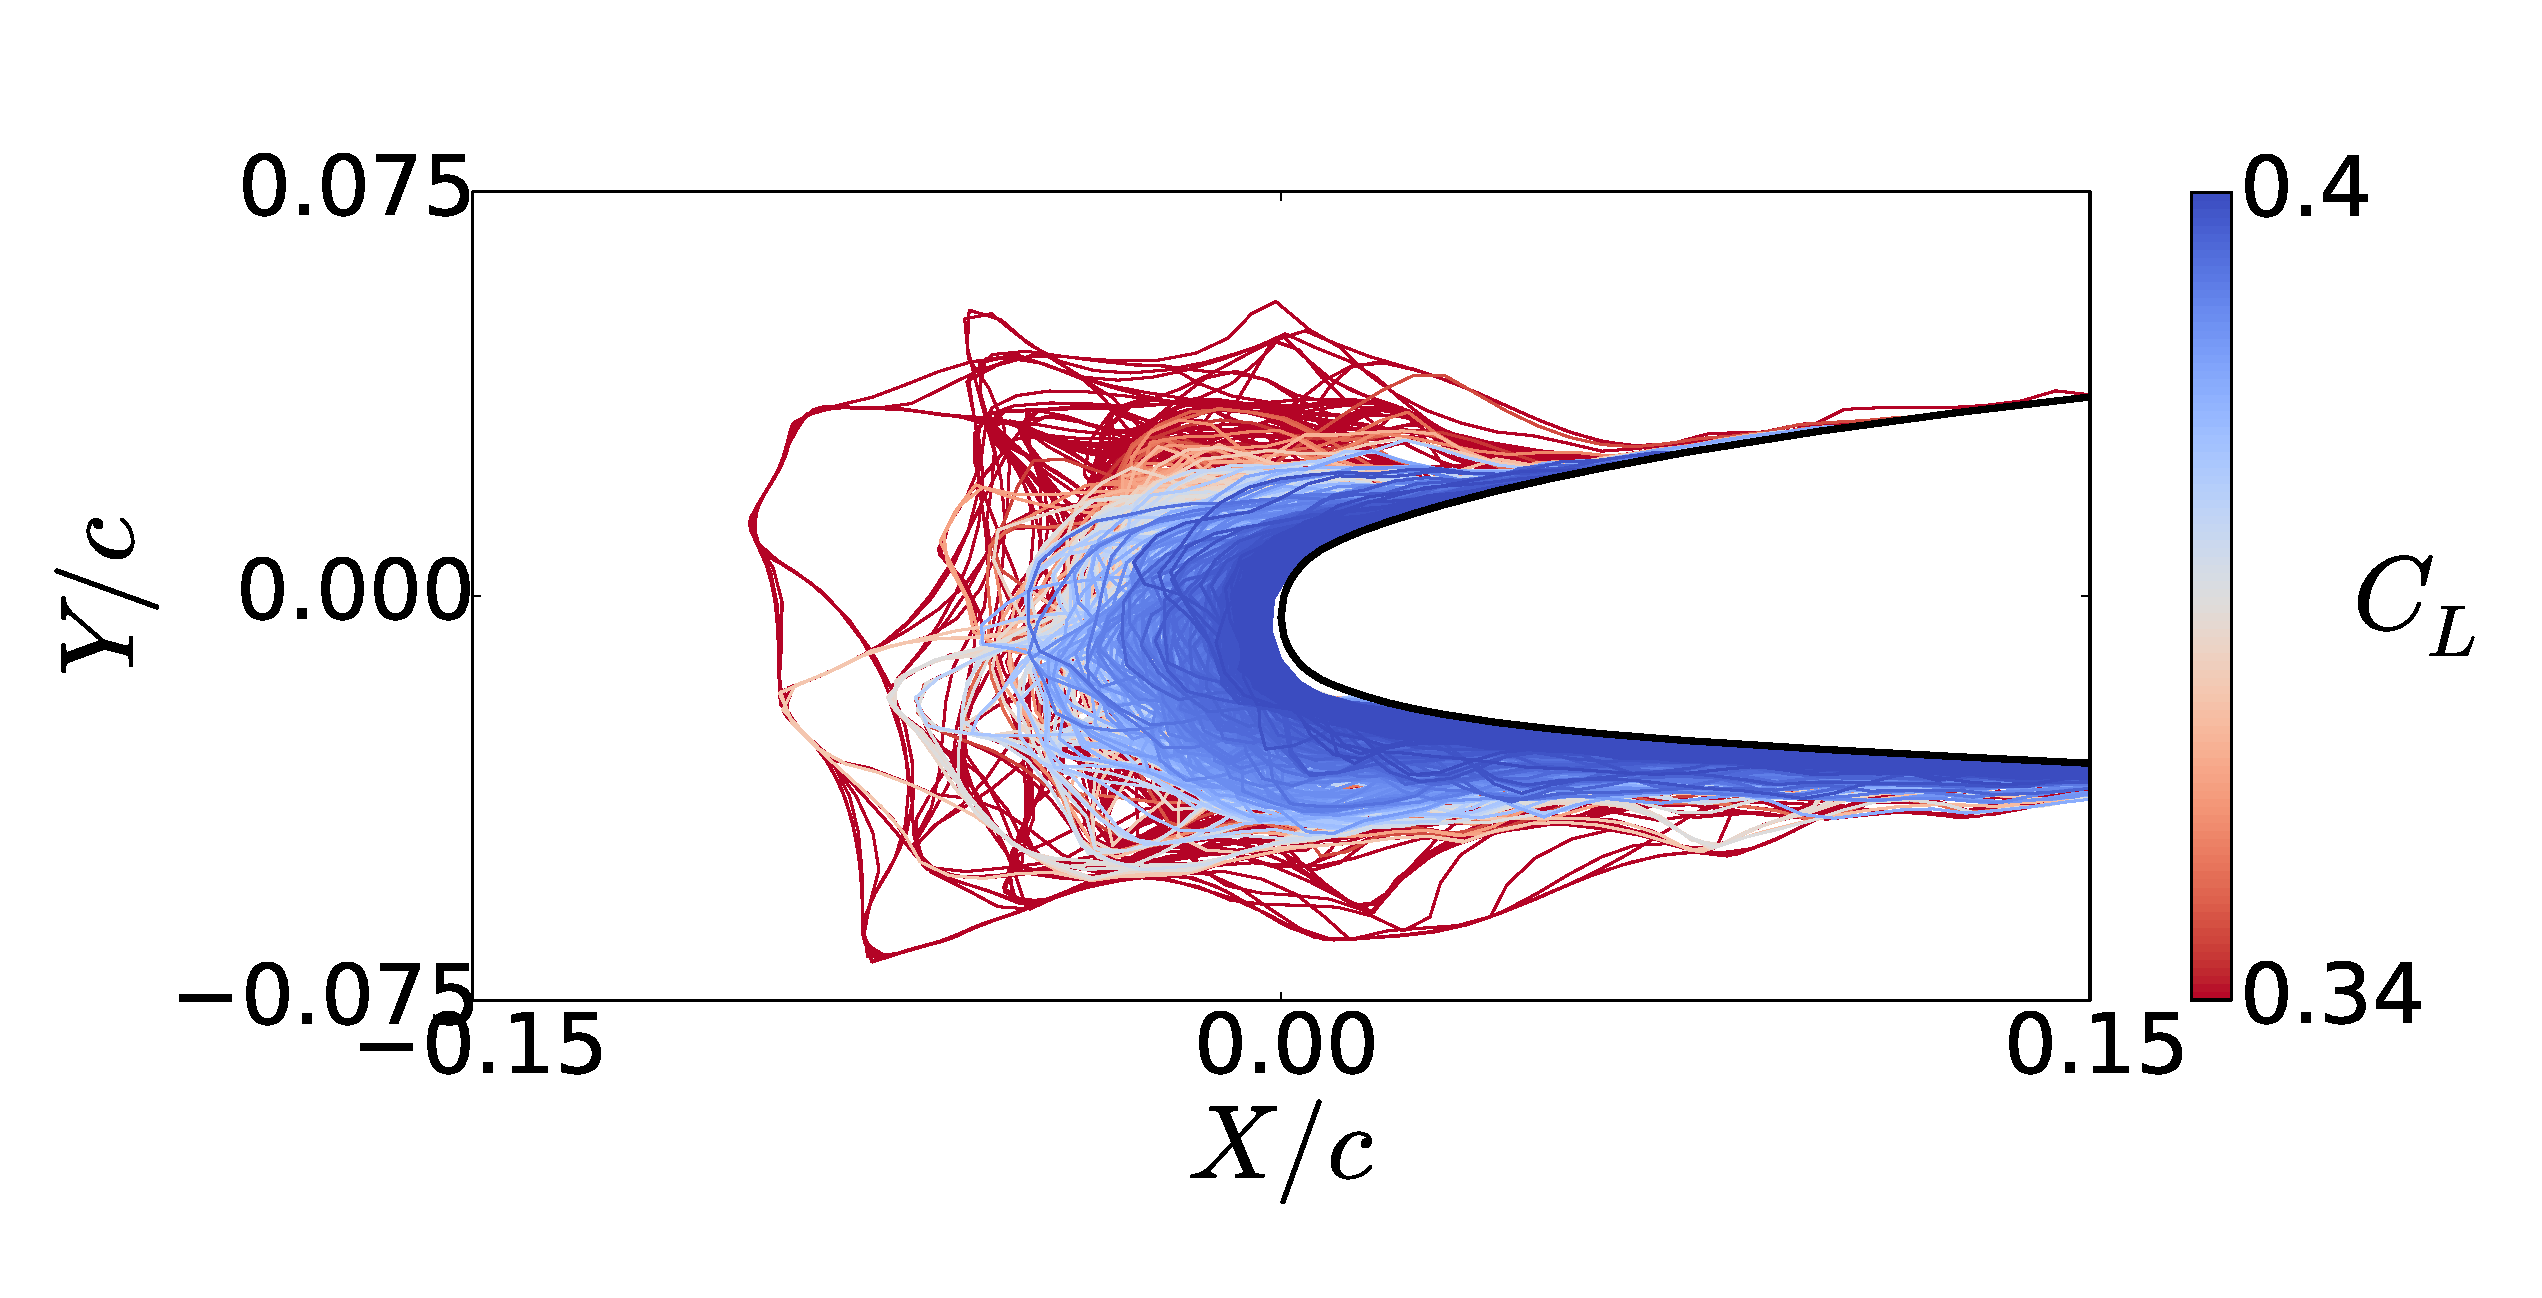
\includegraphics[width=0.6\textwidth]{LHS_Shapes}} \\
      \vspace*{-0.5cm}\subfigure{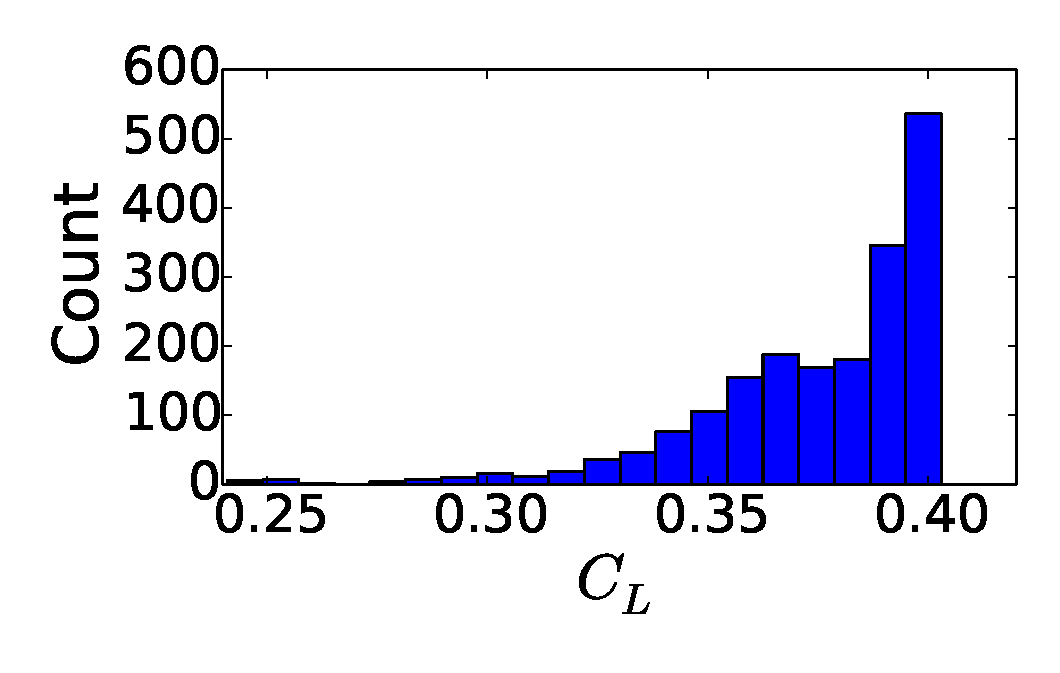
\includegraphics[width=0.35\textwidth]{LHS_Statistics}}
      \vspace*{-0.5cm}\subfigure{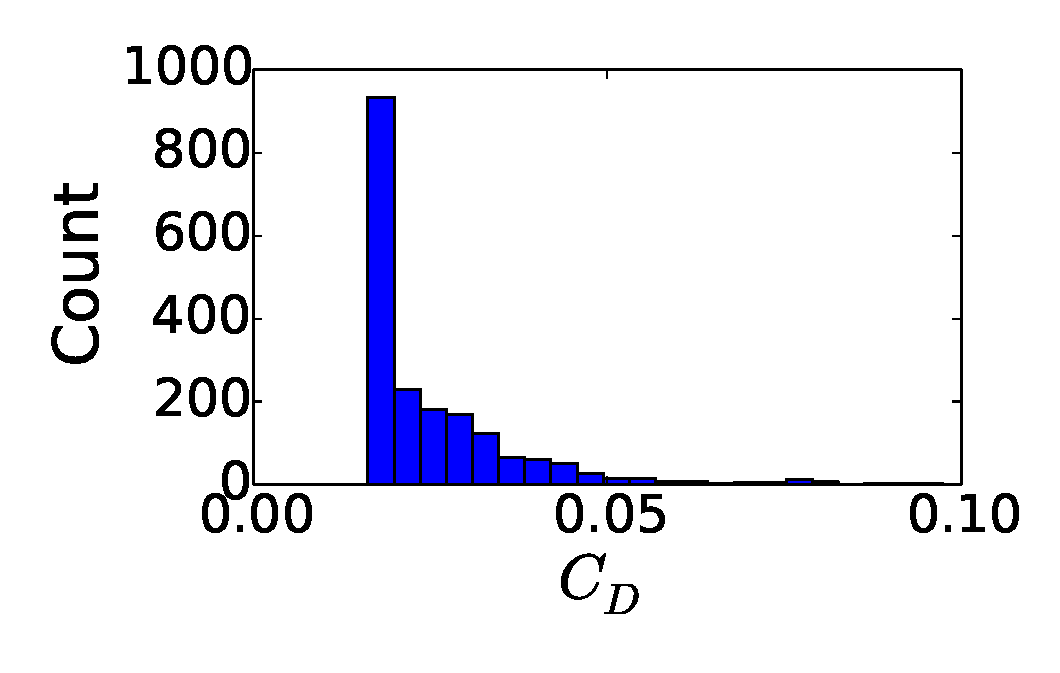
\includegraphics[width=0.35\textwidth]{LHS_StatisticsCD}}
      \caption{Latin Hypercube samples.}
\end{figure}
\begin{itemize}
\item 1,921 LHS samples from 10-D modal space
\item LHS statistics reflect database statistics
\end{itemize}
\end{frame}
\begin{frame}
\frametitle{Latin Hypercube Samples}
\label{sec-2-12}

\vspace*{-0.0cm}\begin{figure}
      \subfigure{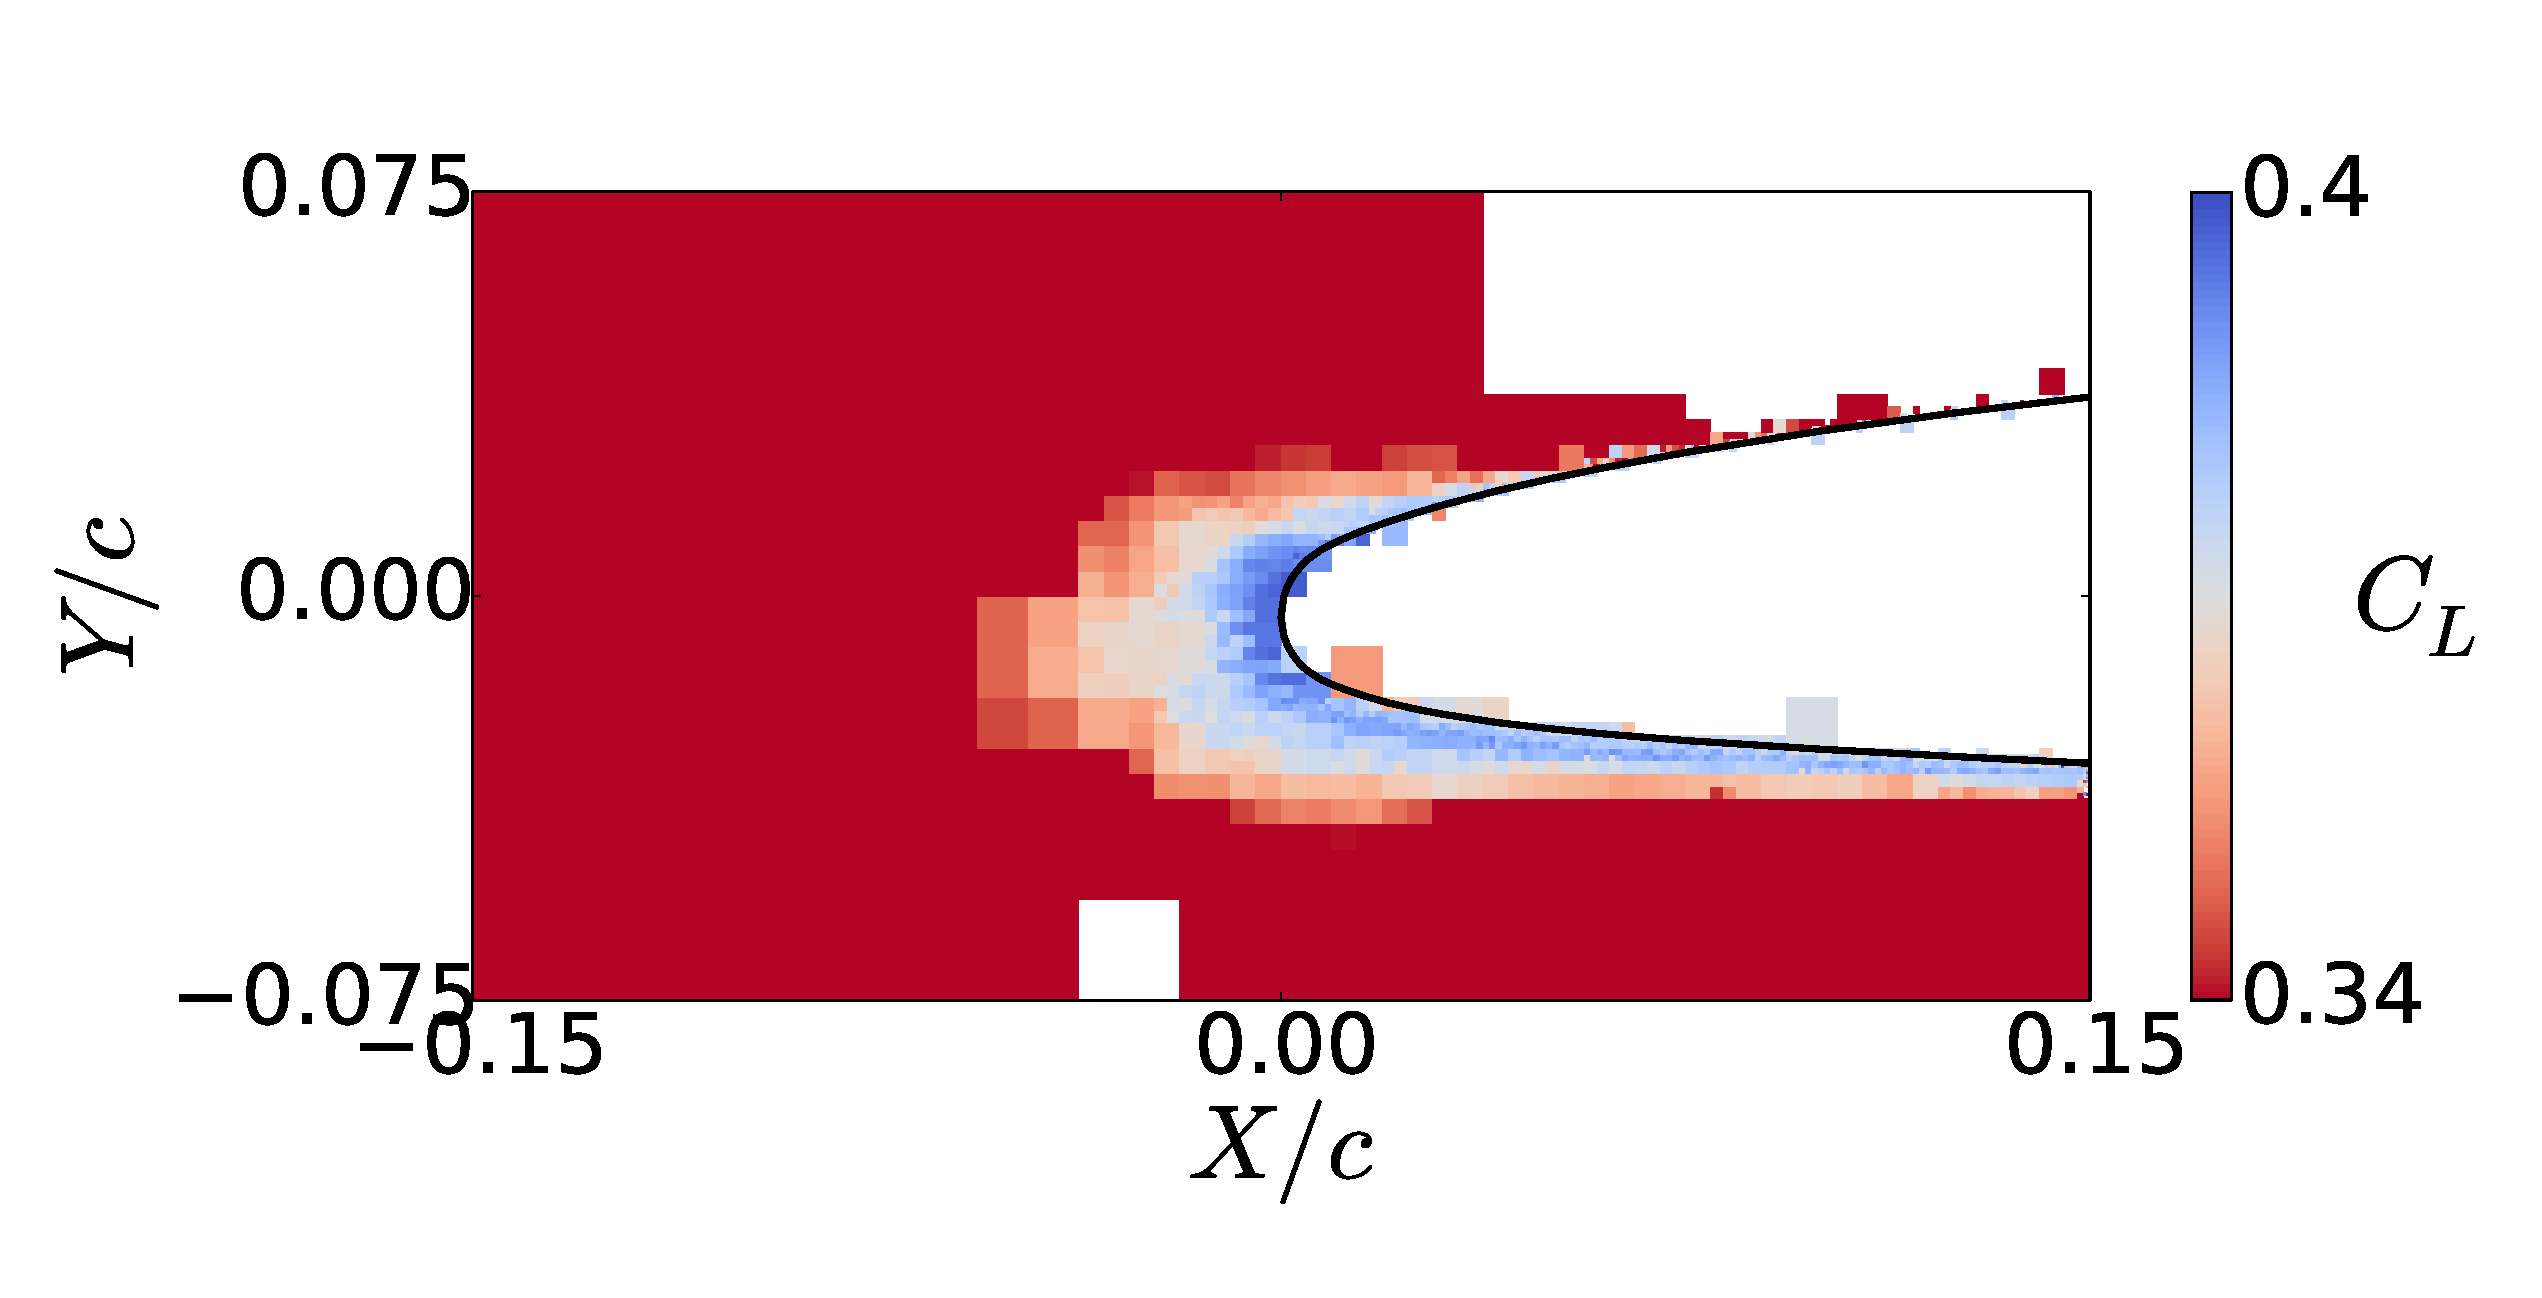
\includegraphics[width=0.45\textwidth]{LHS_SpatialAvg}}
      \subfigure{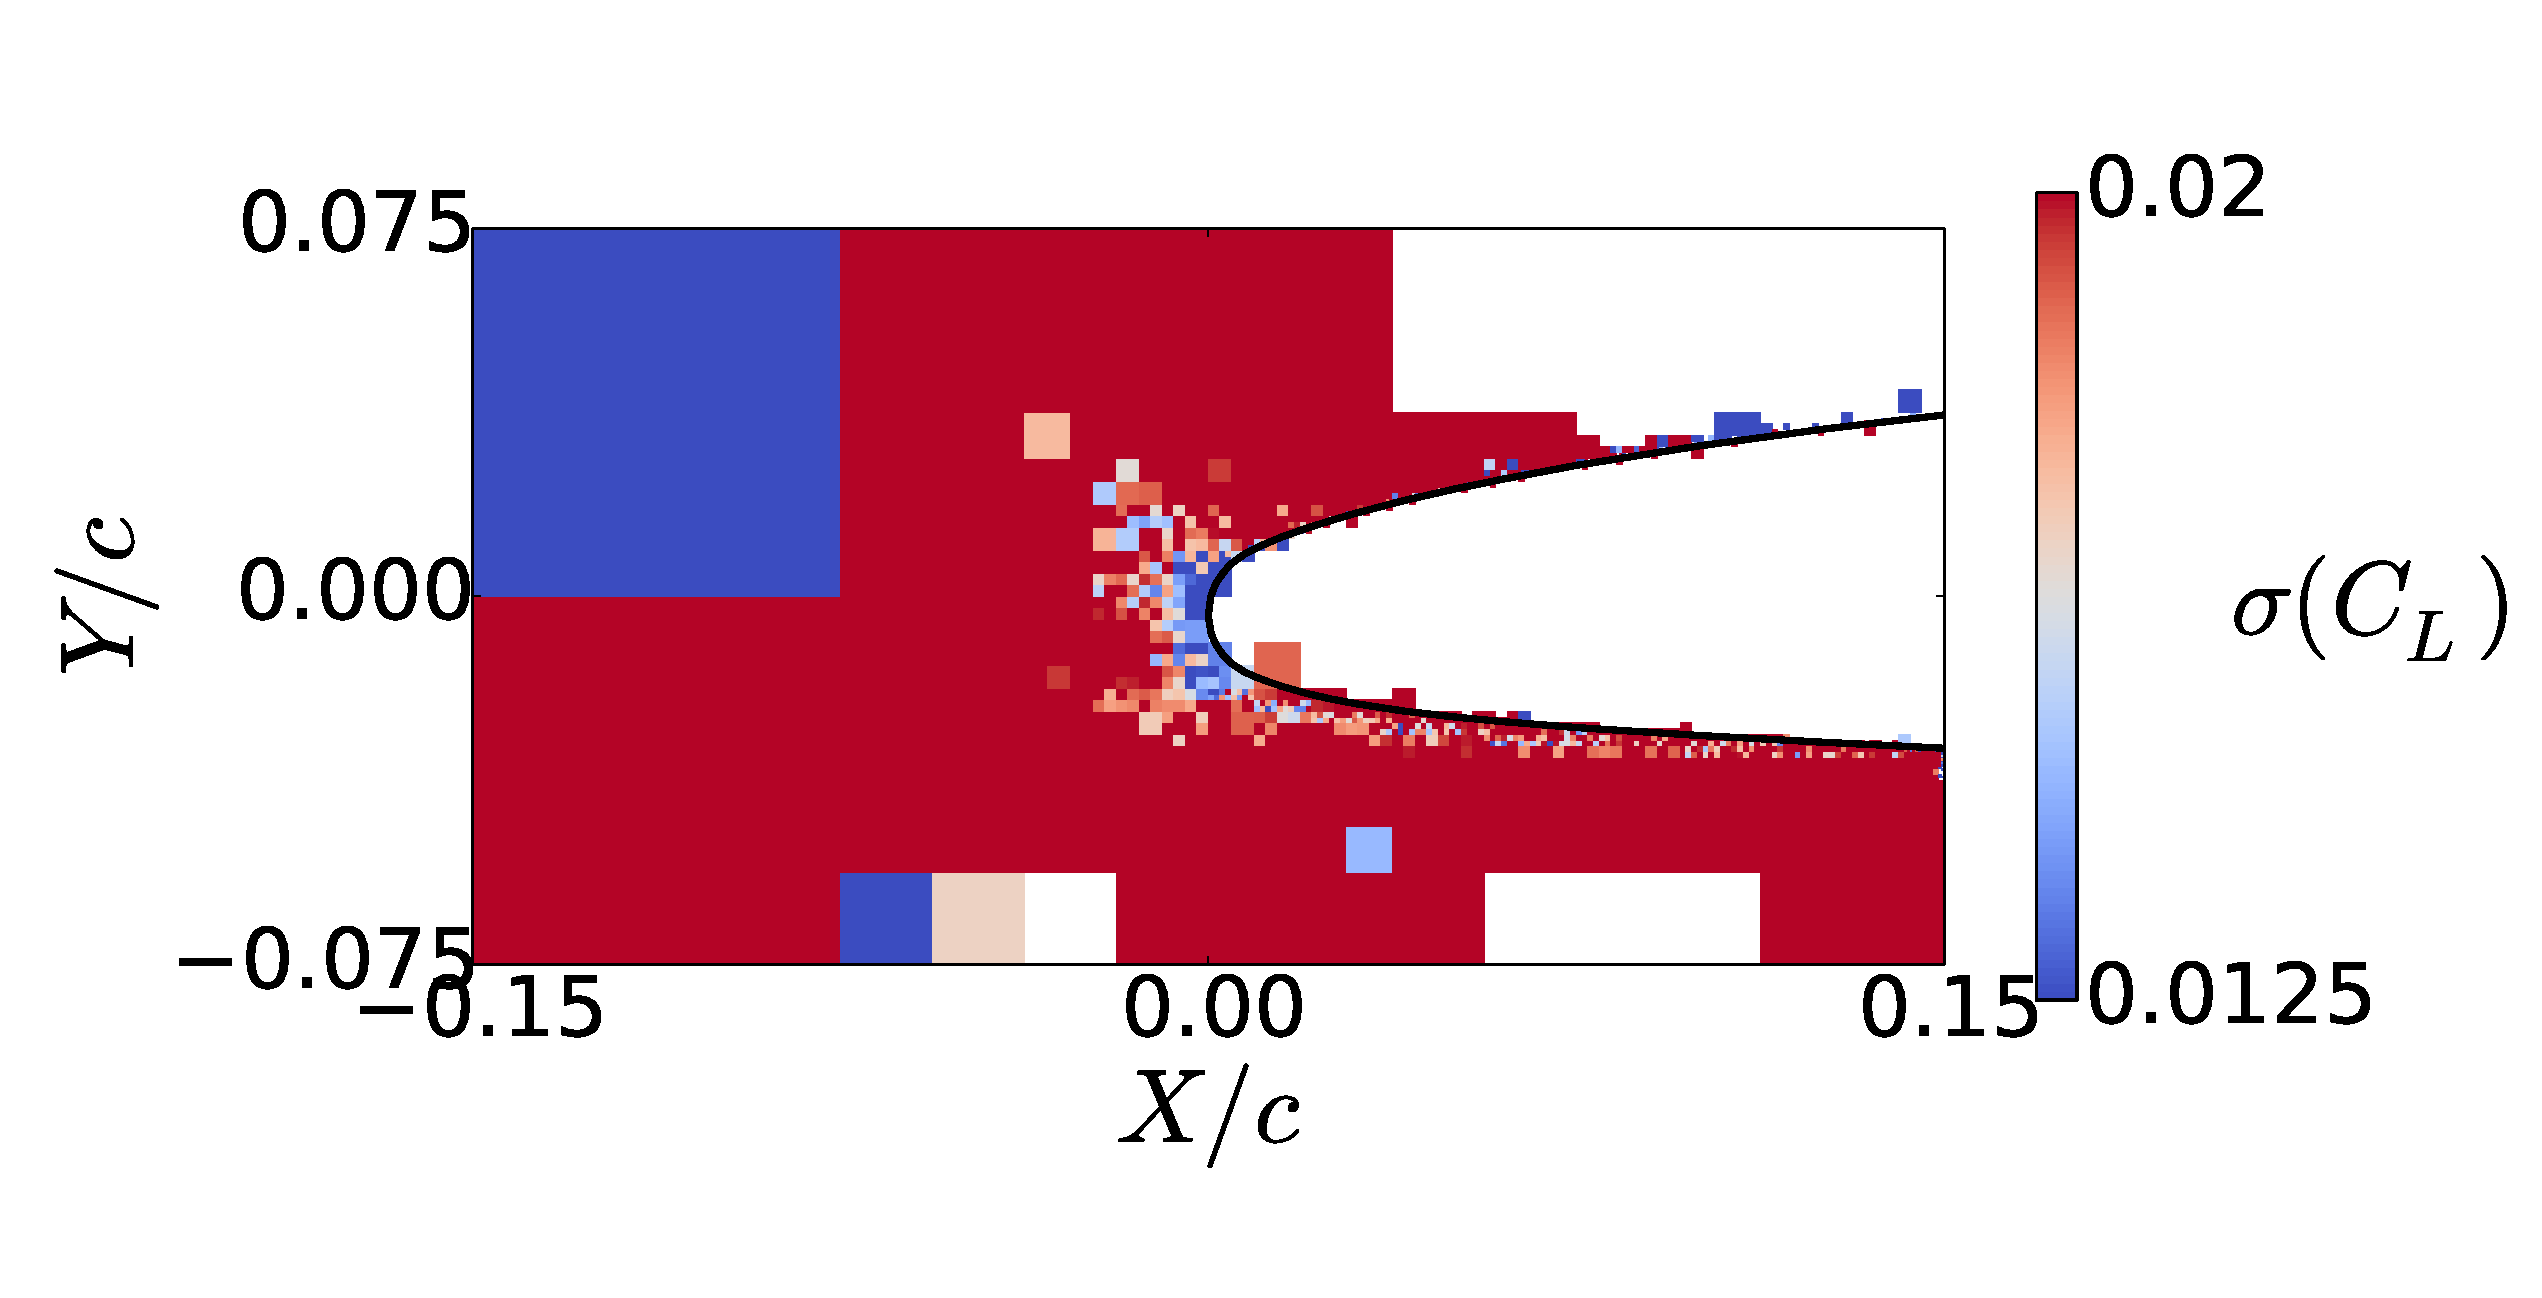
\includegraphics[width=0.45\textwidth]{LHS_SpatialVar}}
      \caption{Spatial average and variance.}
\end{figure}
\begin{itemize}
\item Spatial average: lower surface rime accretions are relatively benign
\item Spatial variance: performance sensitive to upper surface horns
\end{itemize}
\end{frame}
\section{Computational UQ}
\label{sec-3}
\begin{frame}
\frametitle{Motivation}
\label{sec-3-1}

\textbf{Investigate uncertainty in the physical process of icing}
\begin{itemize}
\item What is the statistical effect of uncertainty in physical parameters?
\begin{itemize}
\item Free-stream temperature
\item Liquid water content (LWC)
\item Accretion time
\item Droplet diameter distribution (MVD)
\item Surface roughness
\end{itemize}
\item Want to quantify how perturbations of the physics affects aerodynamics
\end{itemize}
\end{frame}
\begin{frame}
\frametitle{Airfoil Icing Code Flowchart}
\label{sec-3-2}

\fontsize{7}\selectfont
% Define the layers to draw the diagram
\pgfdeclarelayer{background}
\pgfdeclarelayer{foreground}
\pgfsetlayers{background,main,foreground}

\begin{figure}[!ht]
  % Define block styles used later
  \tikzstyle{sensor}=[draw, fill=blue!20, text width=5em, 
    text centered, minimum height=2.5em]
  \tikzstyle{ann} = [above, text width=10em, text centered]
  \tikzstyle{wa} = [sensor, text width=10em, fill=blue!20, 
    minimum height=3em, rounded corners]
  % Define distances for bordering
  %\def\blockdist{2.3}
  %\def\edgedist{2.5}
  \vspace*{-1cm}
  \begin{tikzpicture}

    \begin{pgfonlayer}{background}
      \path (2,4) node (a) {};
      \path (6,-3.5) node (b) {};
      \path[fill=orange!40,rounded corners, draw=black!50, dashed] (a) rectangle (b);
    \end{pgfonlayer}

    \node (CleanAirfoil) [wa] {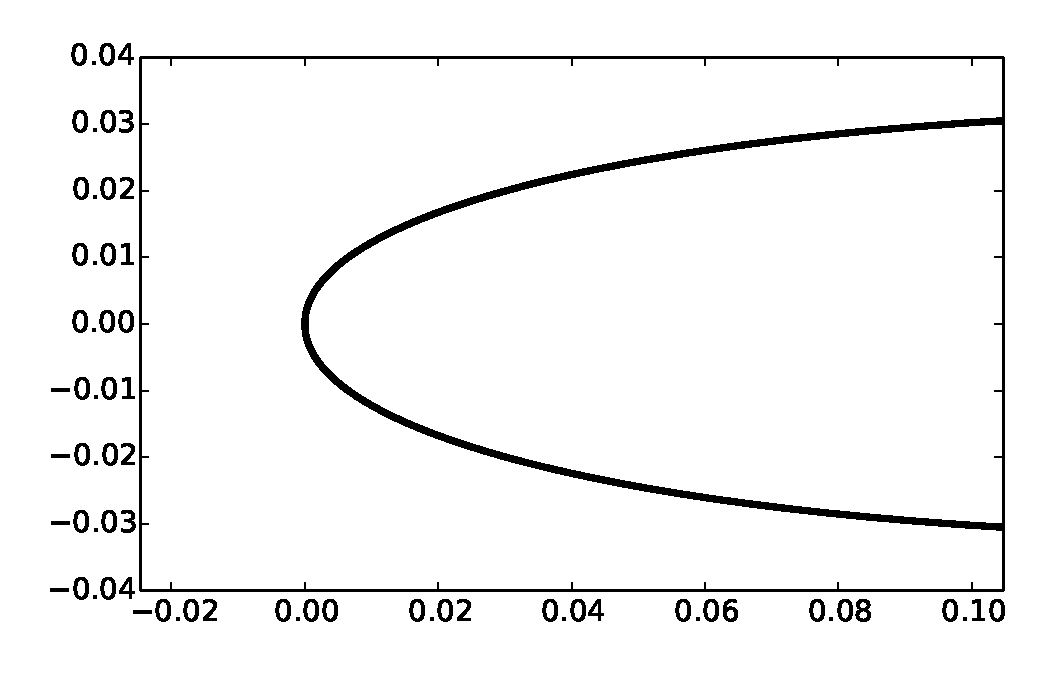
\includegraphics[width=0.6\textwidth]{ExampleCleanAirfoil}\\\bf{Clean Airfoil}};
    \path (CleanAirfoil)+(4,2.5) node (FlowSolver) [wa] {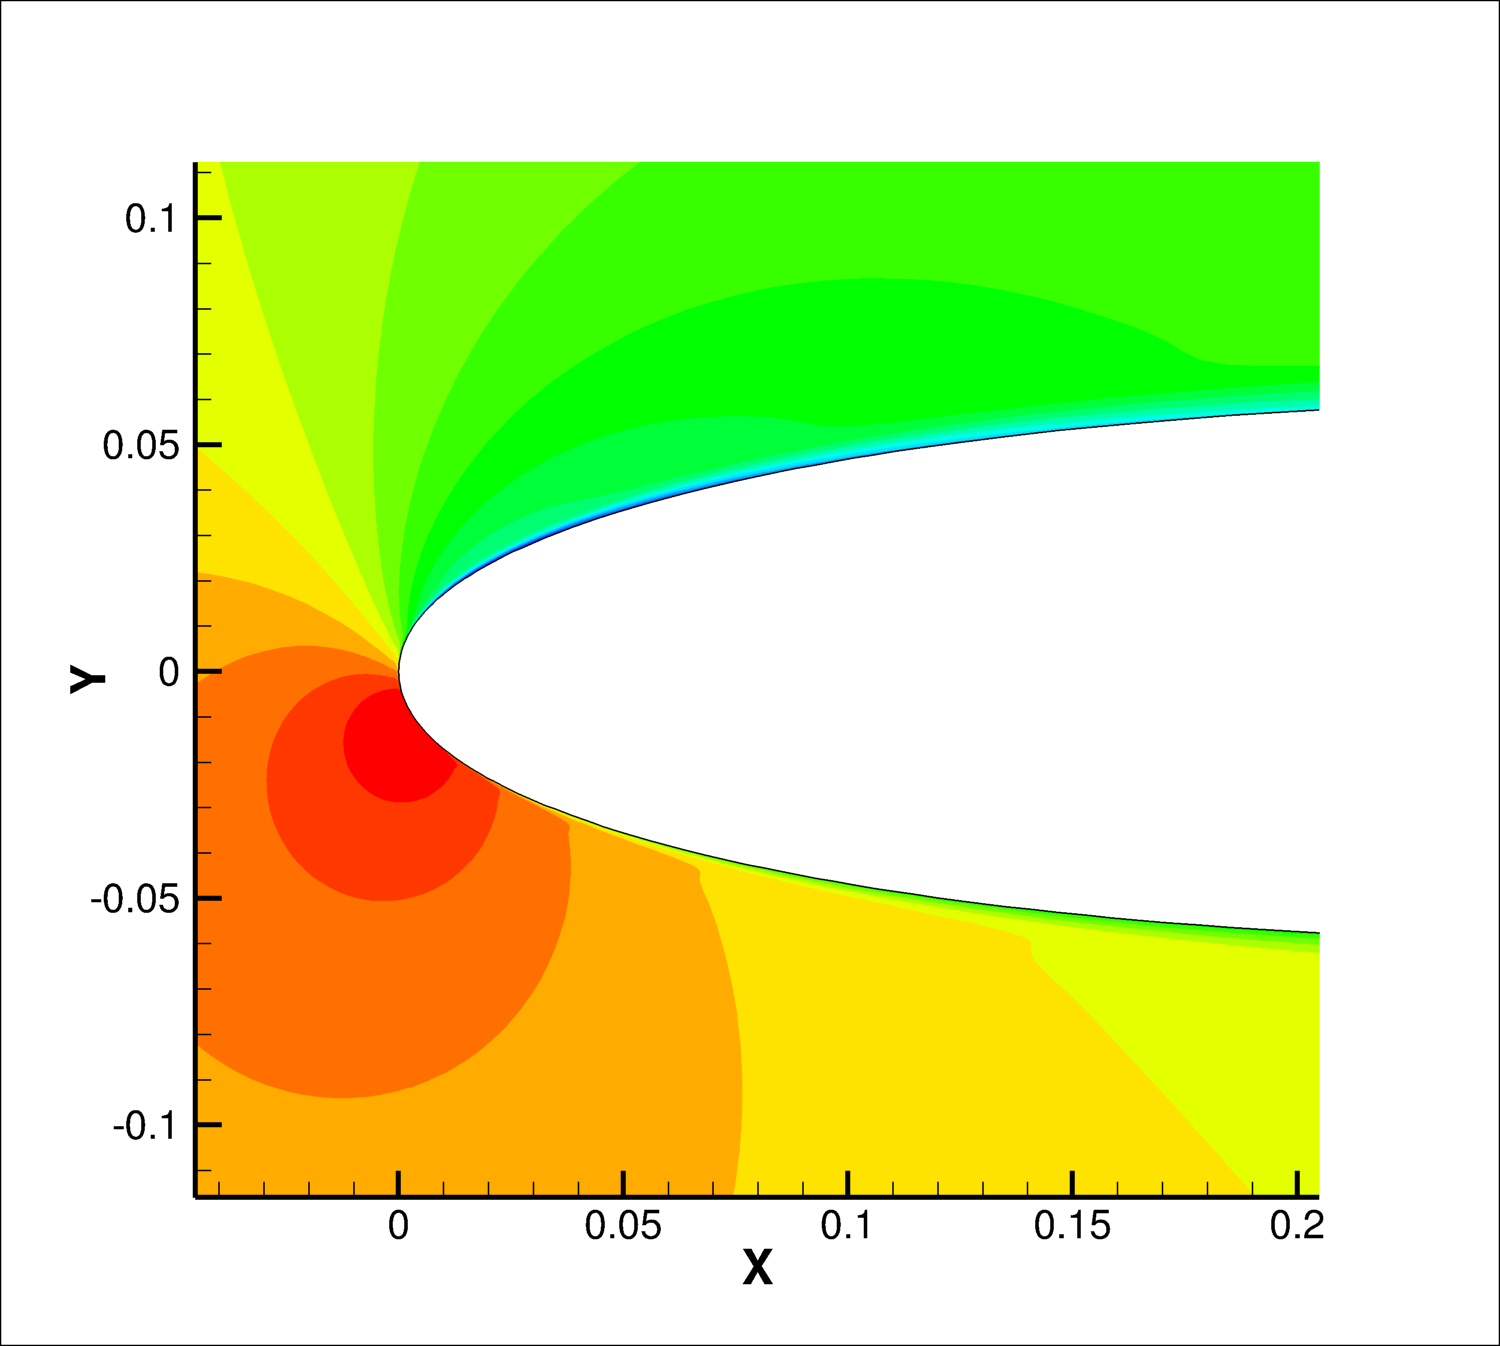
\includegraphics[width=0.6\textwidth]{ExampleSoln}\\\bf{Mesh/Flow Solver}};
    \path (FlowSolver)+(0,-2) node (Droplet) [wa] {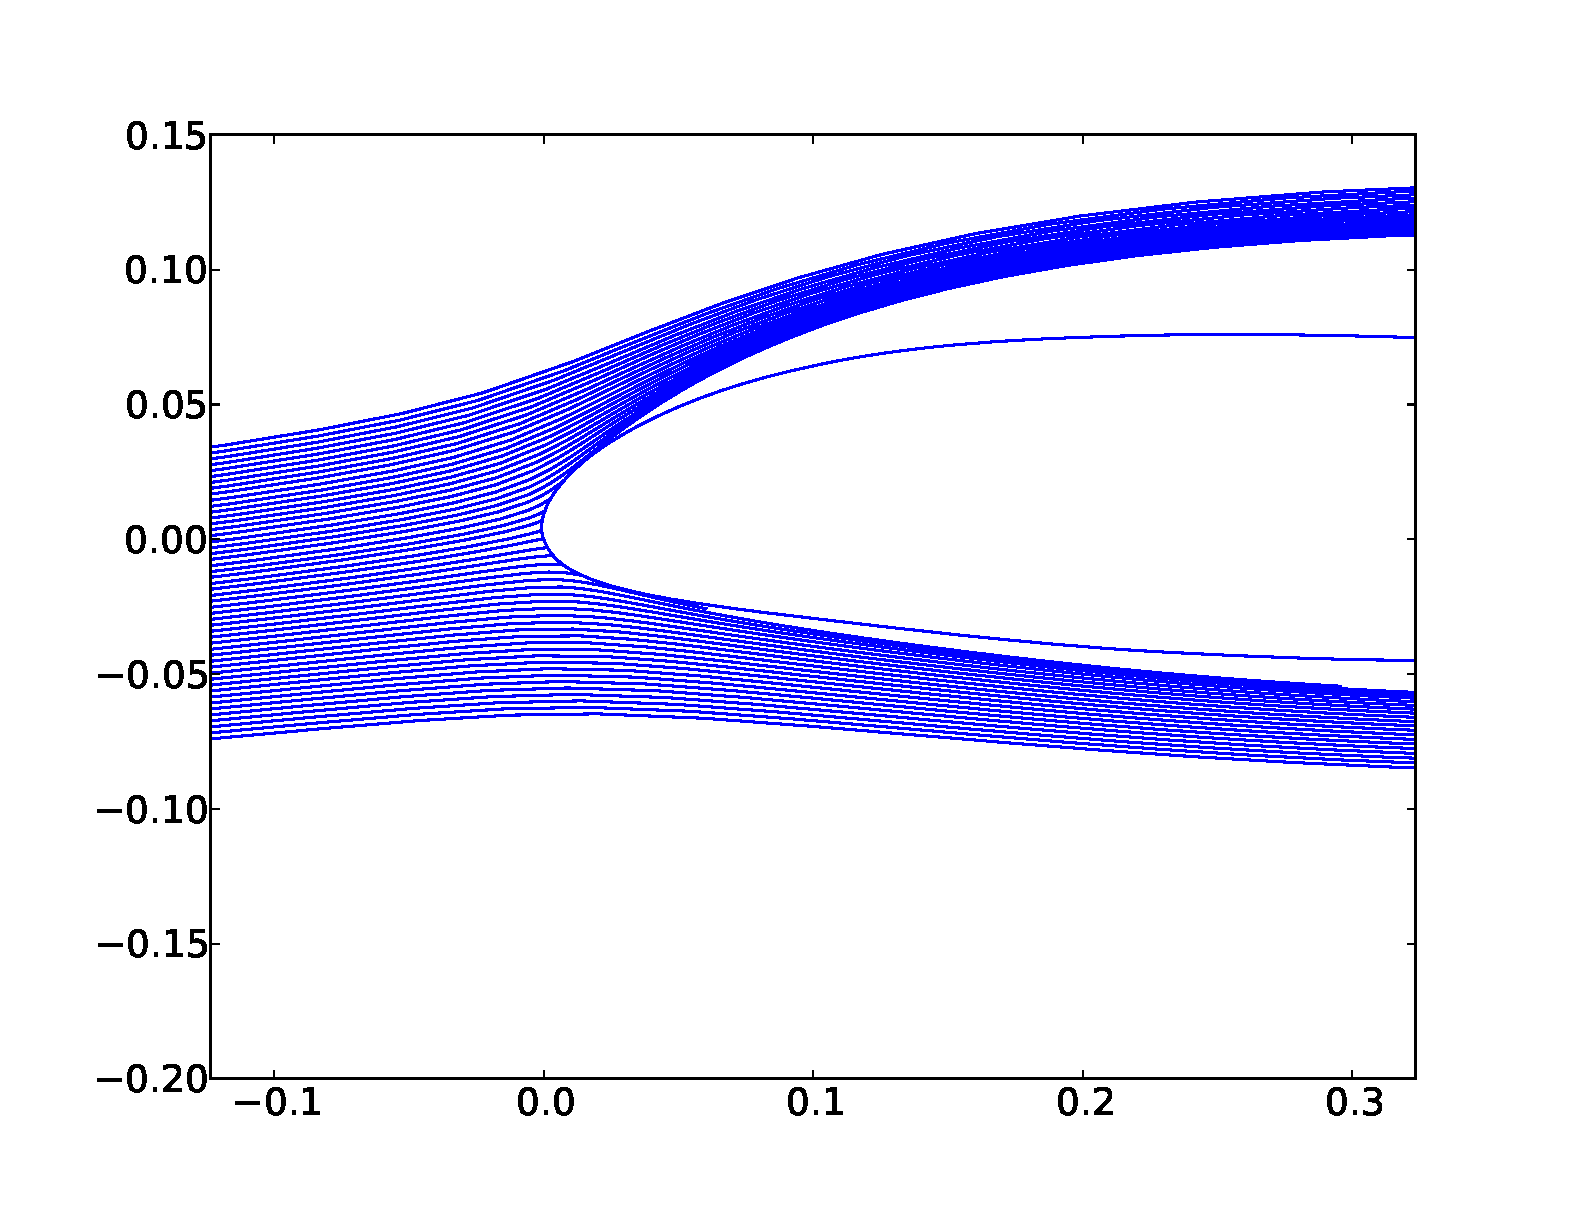
\includegraphics[width=0.6\textwidth]{DropletAdvectionR10}\\\bf{Droplet Simulation}};
    \path (Droplet)+(0,-1.5) node (ThermoModule) [wa] {$\frac{\partial \bm{F}}{\partial t} + \nabla \cdot \bm{F} = \dot{\bm{S}}$ \\\bf{Thermodynamics}};
    \path (ThermoModule)+(0,-1.5) node (IcedAirfoil) [wa] {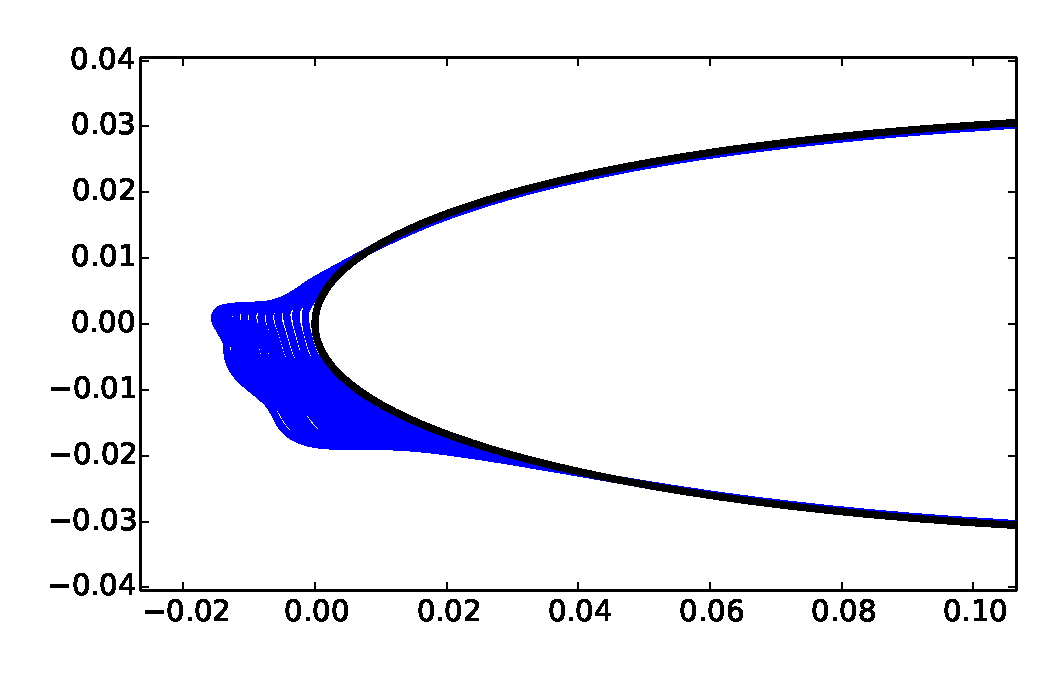
\includegraphics[width=0.6\textwidth]{ExampleIceGrowth}\\\bf{Iced Geometry}};
    \path (CleanAirfoil)+(8,0) node (FinalAirfoil) [wa] {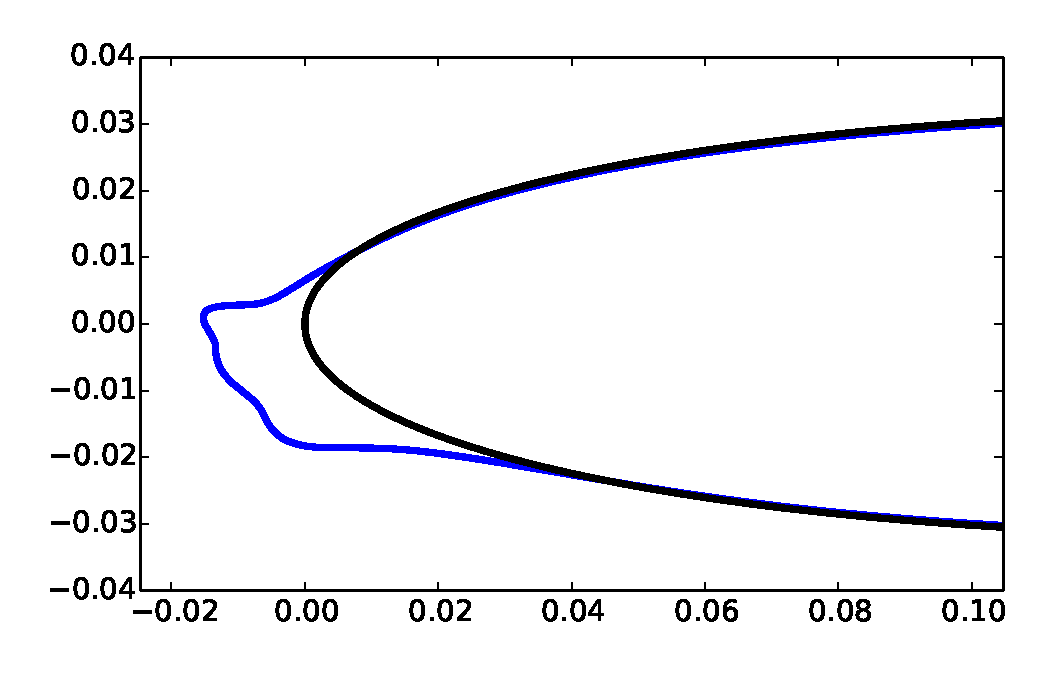
\includegraphics[width=0.6\textwidth]{ExampleIceGrowthFinal}\\\bf{Final Geometry}};

    \path [draw, ->, thick] (CleanAirfoil.north) |- node [above] {} (FlowSolver.west);
    \path [draw, ->, thick] (FlowSolver.south) -- node [below] {} (Droplet.north);
    \path [draw, ->, thick] (Droplet.south) -- node [below] {} (ThermoModule.north);
    \path [draw, ->, thick] (ThermoModule.south) -- node [below] {} (IcedAirfoil.north);
    \path [draw, ->, thick] (IcedAirfoil.east) -| node [above] {} (FinalAirfoil.south);
    \path [draw, ->, thick] (IcedAirfoil.east) -- ++(0.25,0cm) |- node [above]
          {} (FlowSolver.east);

  \end{tikzpicture}

\end{figure}
\end{frame}
\begin{frame}
\frametitle{Droplet Advection}
\label{sec-3-3}

\textbf{Advection Equations:} \\
\begin{equation*}
  \begin{align}
    \frac{d \bv{x}}{d t} &= \bv{v} \\
    m \frac{d \bv{v}}{d t} &= \frac{1}{2} \rho_g C_D \pi r^2 ||\bv{v_g} - \bv{v}|| (\bv{v_g} - \bv{v}) + m \bv{g}
  \end{align}
\end{equation}

\begin{columns}[c]
  \column{0.5\textwidth}
    \centering
    \begin{figure}
    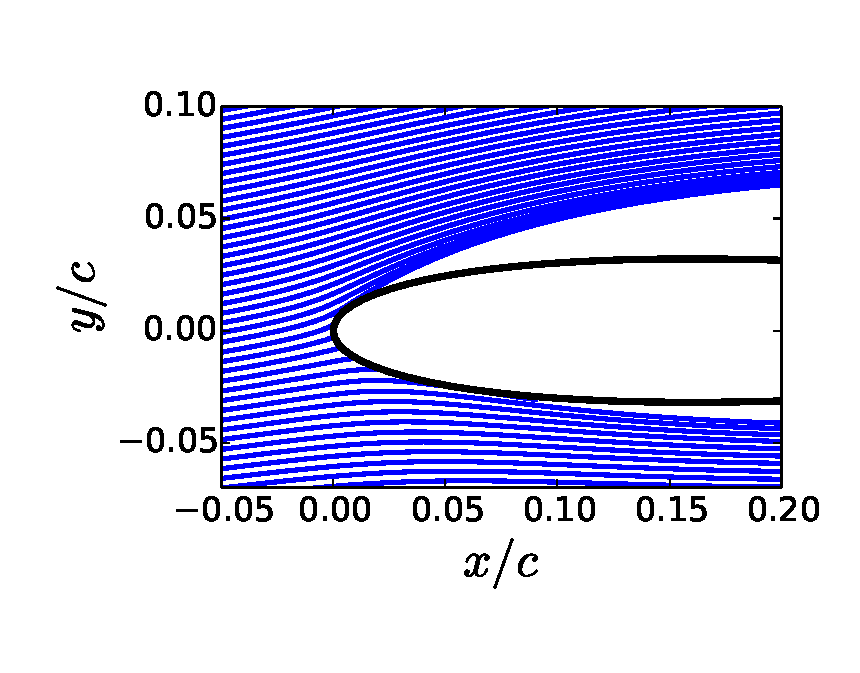
\includegraphics[width=0.9\textwidth]{DropletAdvection_NACA0012_R10}
    \caption{R = 10$\mu$m}
    \end{figure}
  \column{0.5\textwidth}
    \centering
    \begin{figure}
    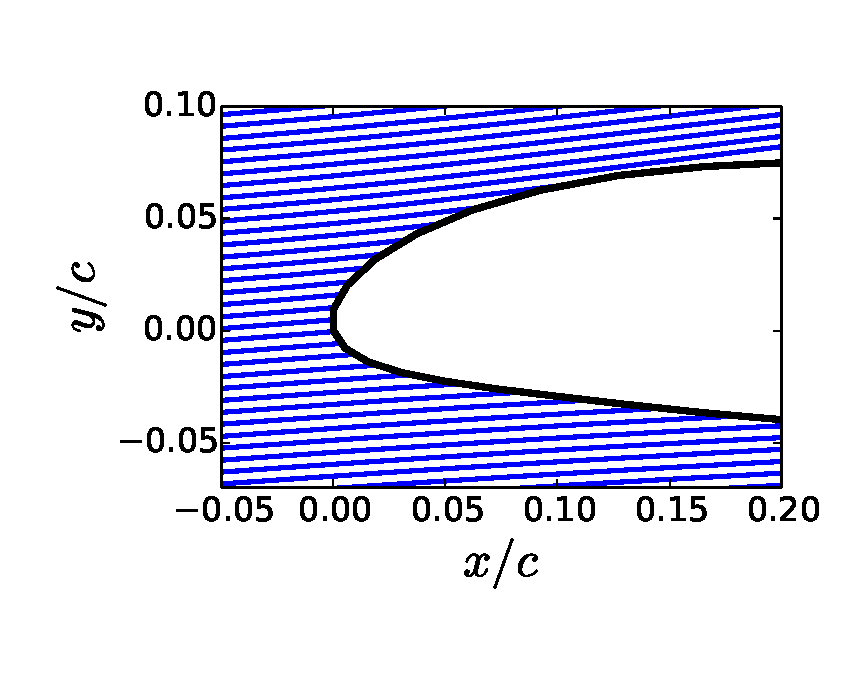
\includegraphics[width=0.9\textwidth]{DropletAdvection_NACA23012_R118} \\
    \caption{R = 118$\mu$m}
    \end{figure}
\end{columns}
\end{frame}
\begin{frame}
\frametitle{Thermodynamics}
\label{sec-3-4}

\textbf{Conservation Equations:} \\
\begin{equation*}
  \begin{align}
    \rho_w \left \lbrace \frac{\partial h_f}{\partial t} + \nabla \cdot (\bv{u_f} h_f) \right \rbrace &= \dot{m}_{imp} - \dot{m}_{evap} - \dot{m}_{ice} \\
    \rho_w \left \lbrace \frac{\partial (h_f c_W T)}{\partial t} + \nabla \cdot (\bv{u_f} h_f c_W T) \right \rbrace &= \left [ c_W T_d + \frac{u_d^2}{2} \right ] \dot{m}_{imp} \\
    & - L_{evap} \dot{m}_{evap} \\
    & +(L_{fus} + c_{ice}T)\dot{m}_{ice} \\
    & + c_H (T_{Rec} - T)
  \end{align}
\end{equation}

\begin{itemize}
\item \textbf{Mass}
\begin{itemize}
\item Enters through impinging droplets
\item Exits via evaporation/sublimation and freezing
\end{itemize}
\item \textbf{Energy}
\begin{itemize}
\item Enters through impinging droplets, freezing of ice
\item Exits via evaporation/sublimation, radiation, convection
\end{itemize}
\item Solution procedure: explicit marching, finite volume discretization
  with upwinded derivatives
\end{itemize}
\end{frame}
\begin{frame}
\frametitle{Thermodynamics Solution Procedure}
\label{sec-3-5}

\begin{columns}[c]
\column{0.4\textwidth}
\hspace*{-0.5cm}
\scalebox{0.8}{
\begin{equation*}
\begin{aligned}
\frac{\partial U}{\partial t} + \frac{\partial F}{\partial s} &= \dot{S} \\
\int_{\mathcal{B}_k} \left( \frac{\partial U}{\partial t} + \frac{\partial F}{\partial s} \right) \;ds &= \int_{\mathcal{B}_k} \dot{S}\; ds \\
\int_{\mathcal{B}_k} \frac{\partial U}{\partial t}\;ds + \left( F_{k+1/2} - F_{k-1/2} \right) &= \int_{\mathcal{B}_k} \dot{S}\; ds \\
\frac{\partial \bar{U}_k}{\partial t} = \mathrlap{\underbrace{ \frac{1}{\Delta s_k} \int_{\mathcal{B}_k} \dot{S}\; ds - \Delta F_k }_{ \delta_u }} \\
\bar{U}_k^{t+\Delta t} &= \bar{U}_k^{t} - \Delta t \delta_u
\end{aligned}
\end{equation}
}
\column{0.6\textwidth}
\centering
\begin{figure}[ht]
  \centering
  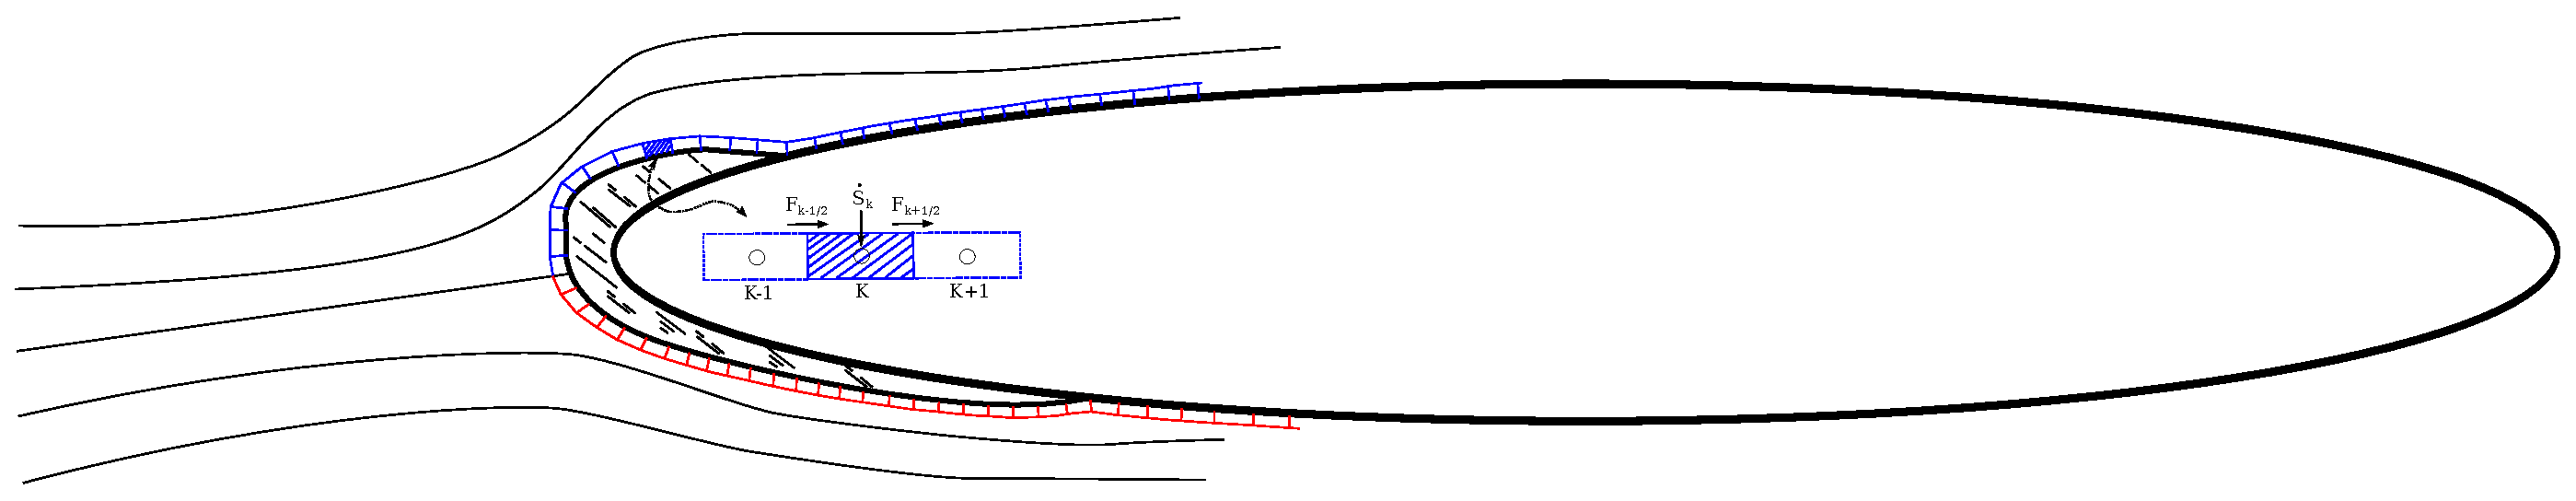
\includegraphics[trim=70mm 20mm 270mm 20mm,clip,width=1\textwidth]{FiniteVolume}
  \caption{Finite volume method.}
\end{figure}
\end{columns}
\begin{itemize}
\item Finite volume discretization of equations
\item Roe scheme flux calculation (upwinding)
\end{itemize}
\end{frame}
\begin{frame}
\frametitle{Validations}
\label{sec-3-6}

\vspace*{-0.5cm}
\begin{figure}[ht]
  \centering
  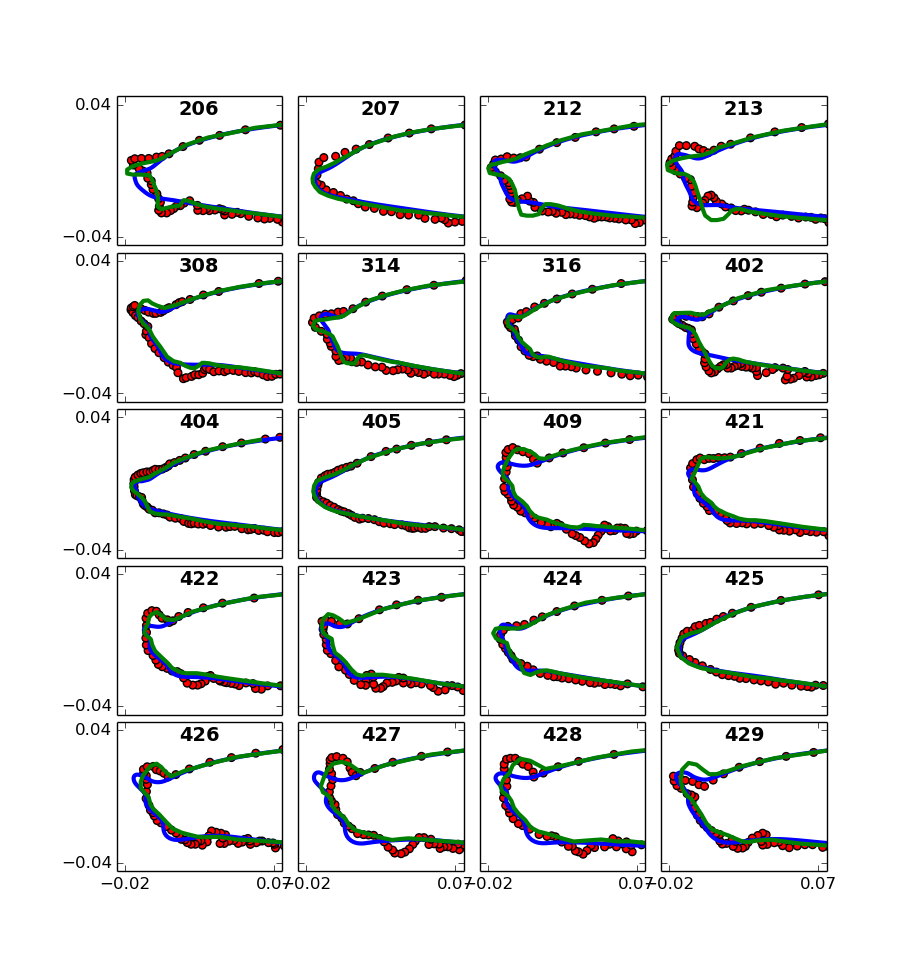
\includegraphics[trim=0.625in 0.75in 0.83in 0.8in,clip,width=0.6\textwidth]{IceShapeValidations.png}
  \caption{Experiment ({\color{red} red}), LEWICE ({\color{green} green}), and CATFISh ({\color{blue} blue}).}
\end{figure}
\end{frame}
\begin{frame}
\frametitle{UQ Study: Temp + LWC}
\label{sec-3-7}

\begin{figure}[ht]
\centering
\subfigure[Quadrature points (colorscale identical to (b)).]{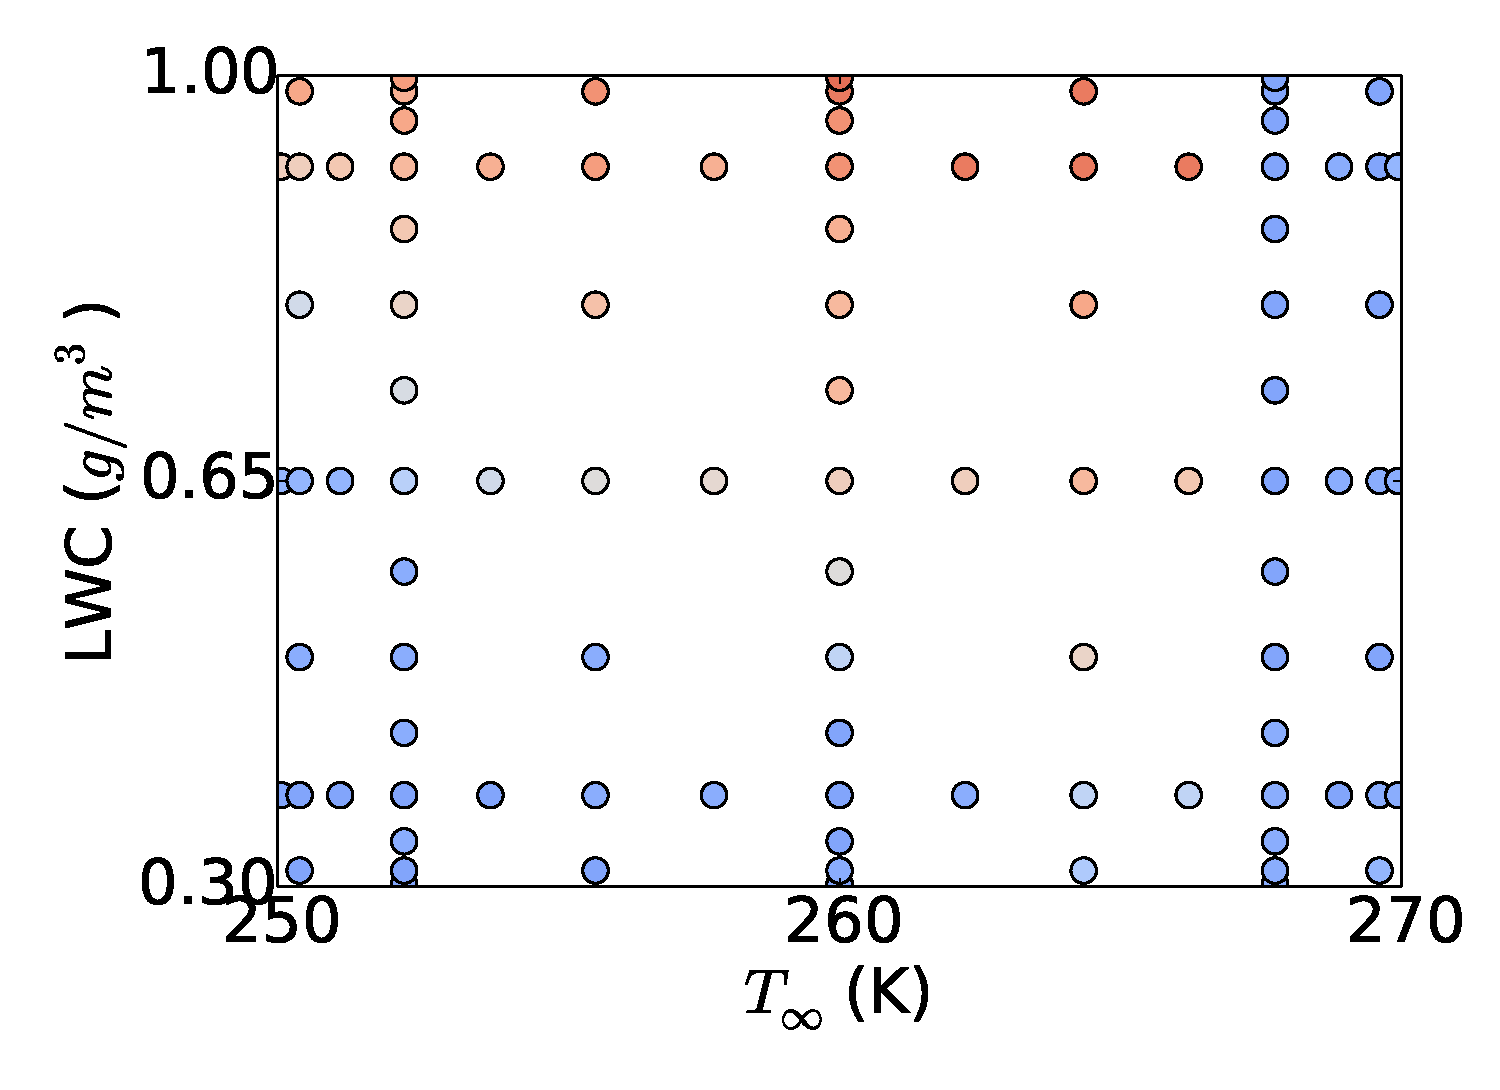
\includegraphics[width=0.3\textwidth]{QuadPts_2ParamCLalpha}}
\subfigure[PCE surrogate.]{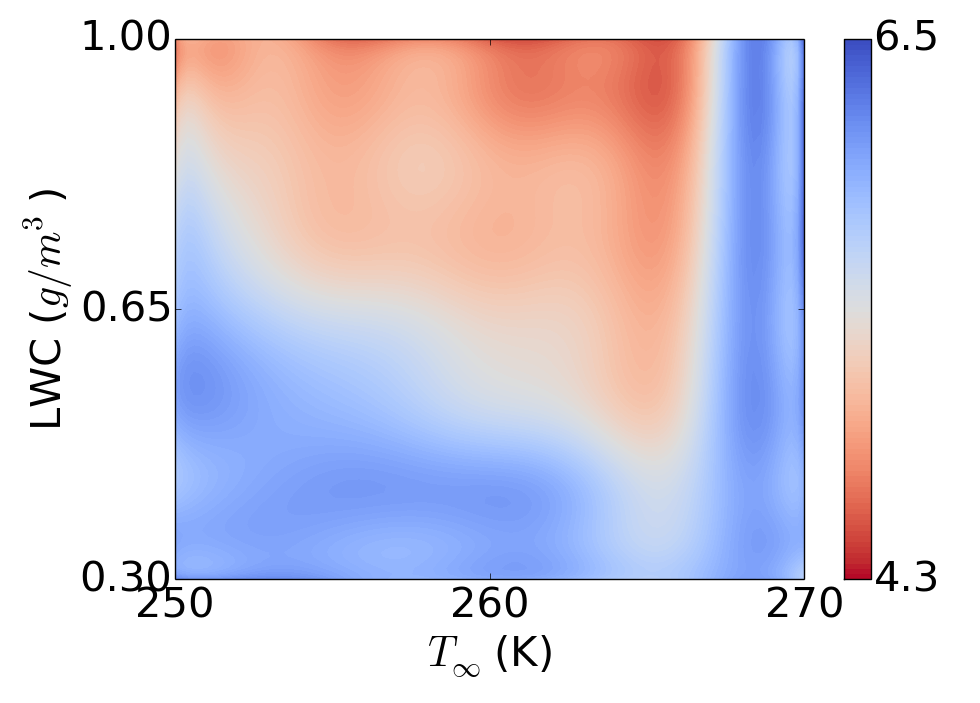
\includegraphics[width=0.3\textwidth]{Map_2ParamCLalpha.png}}
\subfigure[PCE surrogate statistics.]{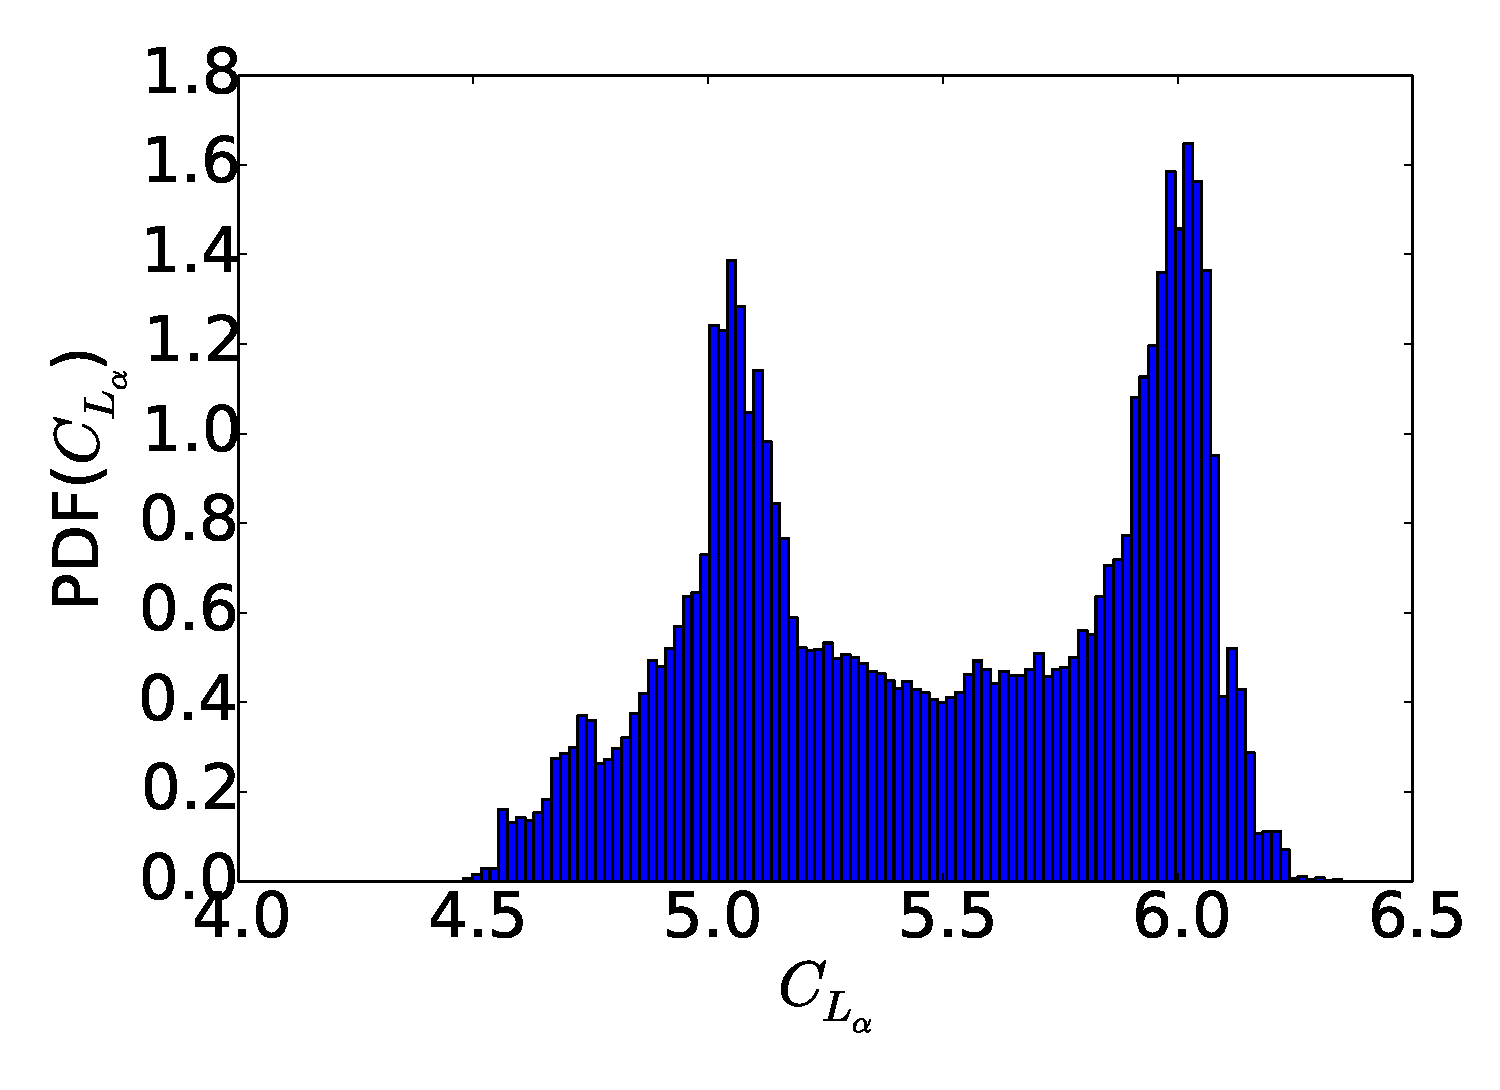
\includegraphics[width=0.3\textwidth]{Statistics_2ParamCLalpha}}
\caption{Quadrature points, PCE surrogate, and statistics for the 2 parameter ($T_{\infty}$ and LWC) study on lift slope.}
\end{figure}
\end{frame}
\begin{frame}
\frametitle{UQ Study: Temp + LWC + Time}
\label{sec-3-8}

\begin{figure}[ht]
\centering
\subfigure[Quadrature points (colorscale identical to (b)).]{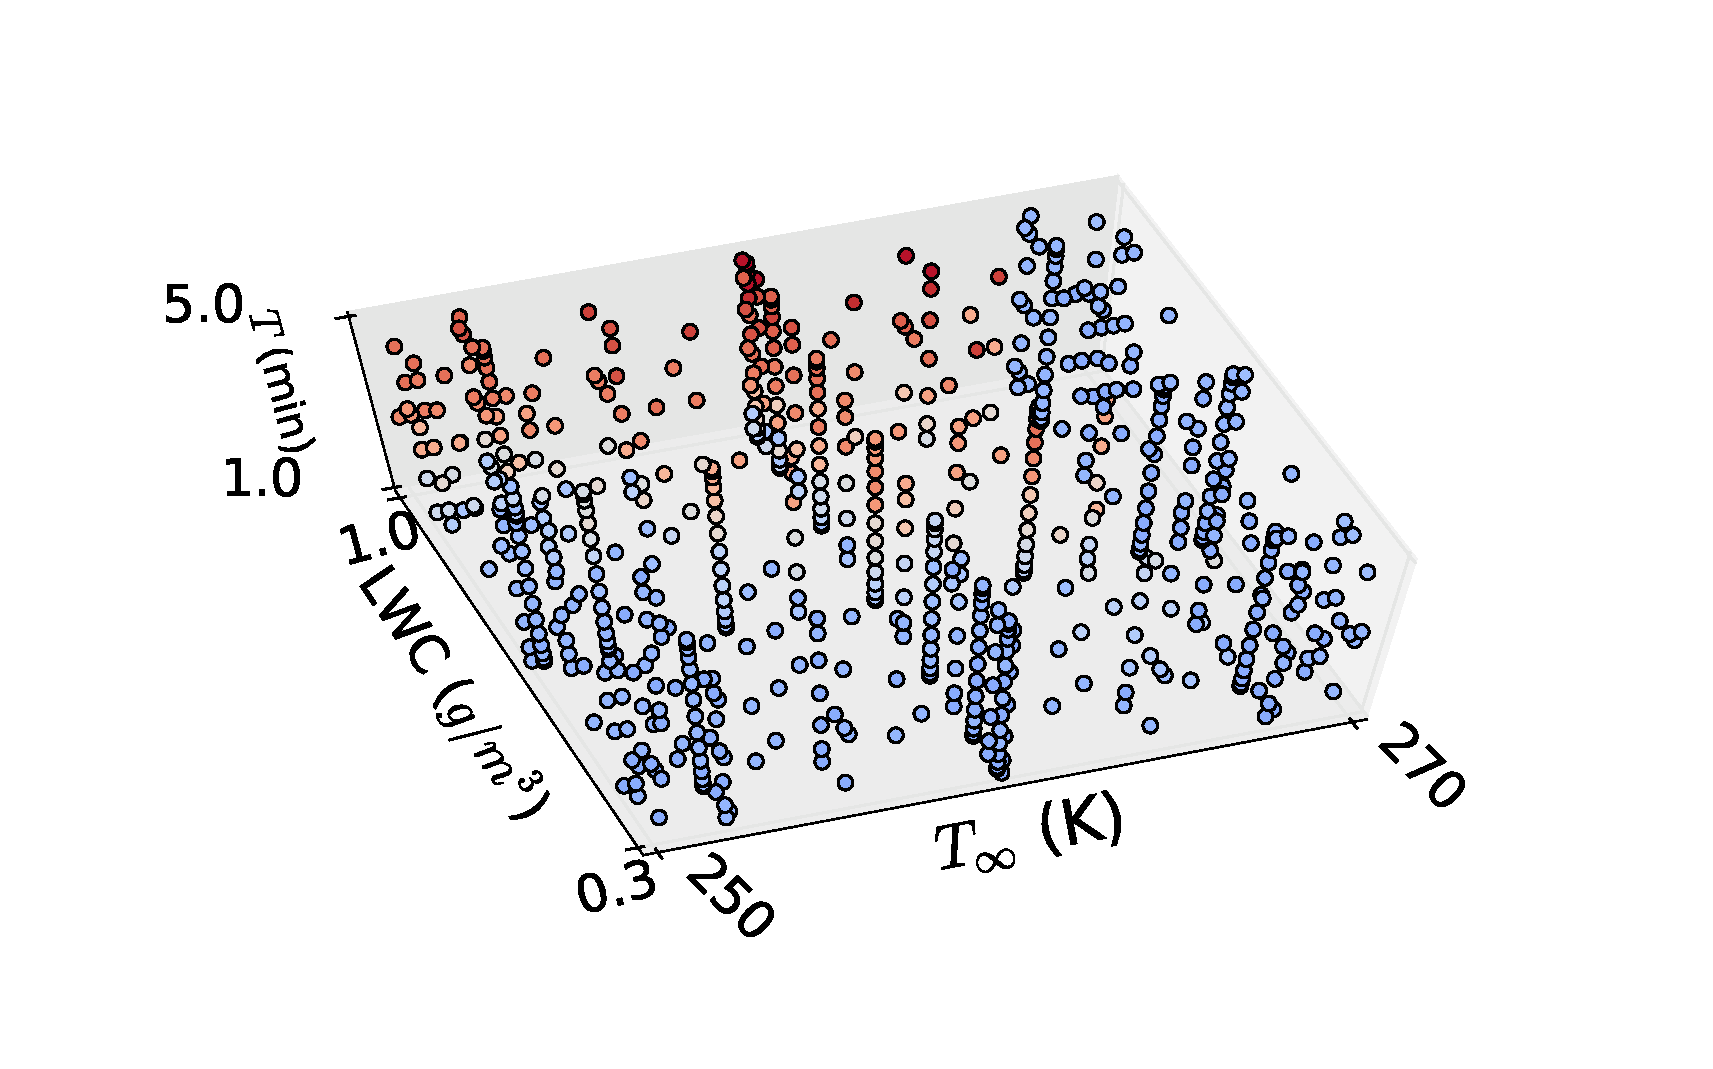
\includegraphics[trim=20mm 0mm 35mm 0mm,clip,width=0.3\textwidth]{3Param_TinfLWCDT_QuadPts}}
\subfigure[PCE surrogate (parameter units identical to (a)).]{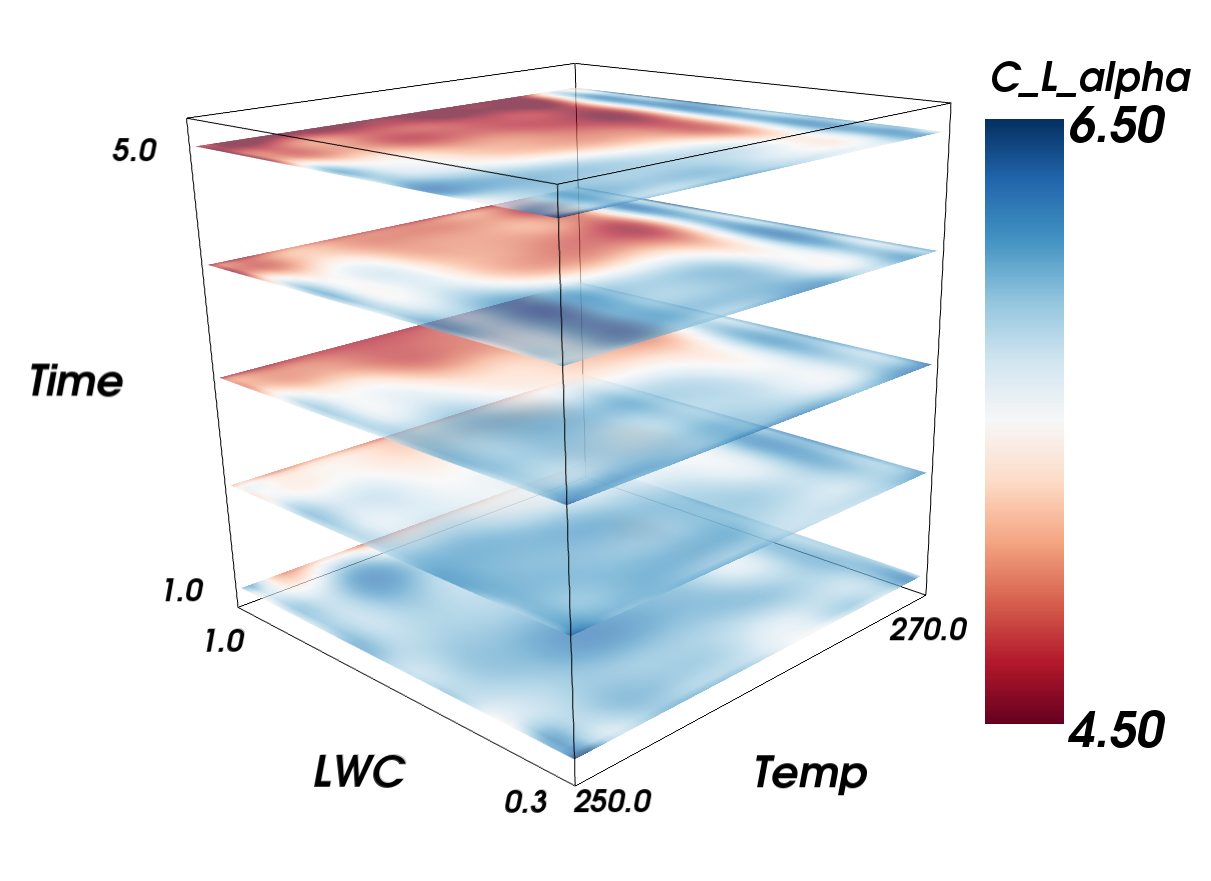
\includegraphics[width=0.3\textwidth]{3Param_TinfLWCDT_Map.png}}
\subfigure[Ice shapes at quadrature points (colorscale identical to (c)).]{\includegraphics[width=0.3\textwidth]{3Param_TinfLWCDT_Shapes}}
\subfigure[PCE surrogate statistics.]{\includegraphics[width=0.3\textwidth]{3Param_TinfLWCDT_Statistics}}
\subfigure[Statistics of $C_{L_{\alpha}}$ as a function of $\Delta$T.]{\includegraphics[width=0.3\textwidth]{3Param_TinfLWCDT_CondExp}}
\caption{Quadrature points, PCE surrogate, and statistics.}
\end{figure}
\end{frame}
\begin{frame}
\frametitle{UQ Study: Temp + LWC + Roughness}
\label{sec-3-9}

\begin{figure}[ht]
\centering
\subfigure[Quadrature points (colorscale identical to (b)).]{\includegraphics[trim=20mm 0mm 35mm 0mm,clip,width=0.3\textwidth]{3Param_TinfLWCRough_QuadPts}}
\subfigure[PCE surrogate (parameter units identical to (a)).]{\includegraphics[width=0.3\textwidth]{3Param_TinfLWCRough_Map.png}}
\subfigure[Ice shapes at quadrature points (colorscale identical to (c)).]{\includegraphics[width=0.3\textwidth]{3Param_TinfLWCRough_Shapes}}
\subfigure[PCE surrogate statistics.]{\includegraphics[width=0.3\textwidth]{3Param_TinfLWCRough_Statistics}}
\subfigure[Statistics of $C_{L_{\alpha}}$ as a function of $\Delta$T.]{\includegraphics[width=0.3\textwidth]{3Param_TinfLWCRough_CondExp}}
\caption{Quadrature points, PCE surrogate, and statistics.}
\end{figure}
\end{frame}
\begin{frame}
\frametitle{Conclusions}
\label{sec-3-10}

\textbf{Problems:}
\begin{itemize}
\item Wing icing deteriorates icing aerodynamics, danger to safe flight
\item Ice shapes are diverse and complex
\item Not clear what the exact aerodynamic effects of different shapes are
\item Would like systematic way of exploring airfoil icing through data
\end{itemize}
\textbf{Solutions:}
\begin{itemize}
\item Data-driven approach
\begin{itemize}
\item Build empirical model of ice accretion from data
\item Perform parametric UQ to quantify range of performance
\end{itemize}
\item Computational approach
\begin{itemize}
\item Build computational ice accretion code from scratch
\item Perform parametric UQ to quantify effects of physics
\end{itemize}
\end{itemize}







 
\end{frame}

\end{document}
